\documentclass[fleqn,10pt]{olplainarticle}
% Use option lineno for line numbers 

\title{Neural Network Exploration}

\author[1]{First Author}
\author[2]{Second Author}
\affil[1]{Address of first author}
\affil[2]{Address of second author}

\keywords{Keyword1, Keyword2, Keyword3}

\begin{abstract}
Please provide an abstract of no more than 300 words. Your abstract should explain the main contributions of your article, and should not contain any material that is not included in the main text. 
\end{abstract}
\usepackage{parskip}
\usepackage{amsthm}
\usepackage{listings}
\usepackage{color}
\usepackage{hyperref}
\usepackage{amsmath}

\definecolor{mygreen}{rgb}{0,0.6,0}
\definecolor{mygray}{rgb}{0.5,0.5,0.5}
\definecolor{mymauve}{rgb}{0.58,0,0.82}

\lstset{ %
  backgroundcolor=\color{white},   % choose the background color
  basicstyle=\footnotesize,        % size of fonts used for the code
  breaklines=true,                 % automatic line breaking only at whitespace
  captionpos=b,                    % sets the caption-position to bottom
  commentstyle=\color{mygreen},    % comment style
  escapeinside={\%*}{*)},          % if you want to add LaTeX within your code
  keywordstyle=\color{blue},       % keyword style
  stringstyle=\color{mymauve},     % string literal style
  frame=single,
  numbers=left, 
  numberstyle=\small, 
  numbersep=8pt, 
}

\theoremstyle{definition}
\newtheorem{definition}{Definition}[section]
 
\theoremstyle{remark}
\newtheorem*{remark}{Remark}

\newtheorem{theorem}{Theorem}

\begin{document}

\flushbottom
\maketitle
\thispagestyle{empty}
\raggedbottom

\section*{Introduction}
When you look at all these polls, there's a lot of them, but there's only so many organizations, copanies, universities, whatever, that're actually running polls. So after a while, you start to get a little used to the same names coming over and over again. One of them is the L.A. 



Thanks for using Overleaf to write your article. Your introduction goes here! Some examples of commonly used commands and features are listed below, to help you get started.

\section*{Methods and Materials}

Guidelines can be included for standard research article sections, such as this one.

\section*{Some \LaTeX{} Examples}
\label{sec:examples}

Use section and subsection commands to organize your document. \LaTeX{} handles all the formatting and numbering automatically. Use ref and label commands for cross-references.

\subsection*{Figures and Tables}

Use the table and tabular commands for basic tables --- see Table~\ref{tab:widgets}, for example. You can upload a figure (JPEG, PNG or PDF) using the project menu. To include it in your document, use the includegraphics command as in the code for Figure~\ref{fig:view} below.

\begin{figure}[ht]
\centering

\includegraphics[width=0.7\linewidth]{frog}
\caption{An example image of a frog.}
\label{fig:view}
\end{figure}

\begin{table}[ht]
\centering
\begin{tabular}{l|r}
Item & Quantity \\\hline
Candles & 4 \\
Fork handles & ?  
\end{tabular}
\caption{\label{tab:widgets}An example table.}
\end{table}

\subsection*{Citations}

LaTeX formats citations and references automatically using the bibliography records in your .bib file, which you can edit via the project menu. Use the cite command for an inline citation, like \cite{lees2010theoretical}, and the citep command for a citation in parentheses \citep{lees2010theoretical}.

\subsection*{Mathematics}

\LaTeX{} is great at typesetting mathematics. Let $X_1, X_2, \ldots, X_n$ be a sequence of independent and identically distributed random variables with $\text{E}[X_i] = \mu$ and $\text{Var}[X_i] = \sigma^2 < \infty$, and let
$$S_n = \frac{X_1 + X_2 + \cdots + X_n}{n}
      = \frac{1}{n}\sum_{i}^{n} X_i$$
denote their mean. Then as $n$ approaches infinity, the random variables $\sqrt{n}(S_n - \mu)$ converge in distribution to a normal $\mathcal{N}(0, \sigma^2)$.

\subsection*{Lists}

You can make lists with automatic numbering \dots

\begin{enumerate}[noitemsep] 
\item Like this,
\item and like this.
\end{enumerate}
\dots or bullet points \dots
\begin{itemize}[noitemsep] 
\item Like this,
\item and like this.
\end{itemize}
\dots or with words and descriptions \dots
\begin{description}
\item[Word] Definition
\item[Concept] Explanation
\item[Idea] Text
\end{description}

\section*{Acknowledgments}

Additional information can be given in the template, such as to not include funder information in the acknowledgments section.

\bibliography{sample}

\clearpage
\section*{Lesson 8: Eigenvectors}
One of the nicer way (according to Shewchuk) to look at and understand eigenvectors of symmetric matrices is by looking at a quadratic curve called the quadratic form that comes out of it. To remind you, here's the definition of a eigenvector:


\theoremstyle{definition}
\begin{definition}{\textbf{Eigenvector}}
Given matrix $A$, if $Av = \lambda v$, for some vector $v \neq 0$ and $\lambda$ is a scalar, \\ then $v$ is an \underline{eigenvector} of $A$.
\end{definition}

So this is the definition you learned in your Linear Algebra class or whatever. But what does it really mean? So what that $Av = \lambda v$ means is there's a special vector $v$ that when I multiply it by $A$, it still points at the same direction or in the opposite direction, but the line through that vector has not changed at all. 

Let's look at a couple examples. I'm gonna draw four coordinate systems here, and it these coordinate systems, I'm gonna put a eigenvector $v$ whose eigenvalue is 2. 

\begin{figure}[ht]
\centering
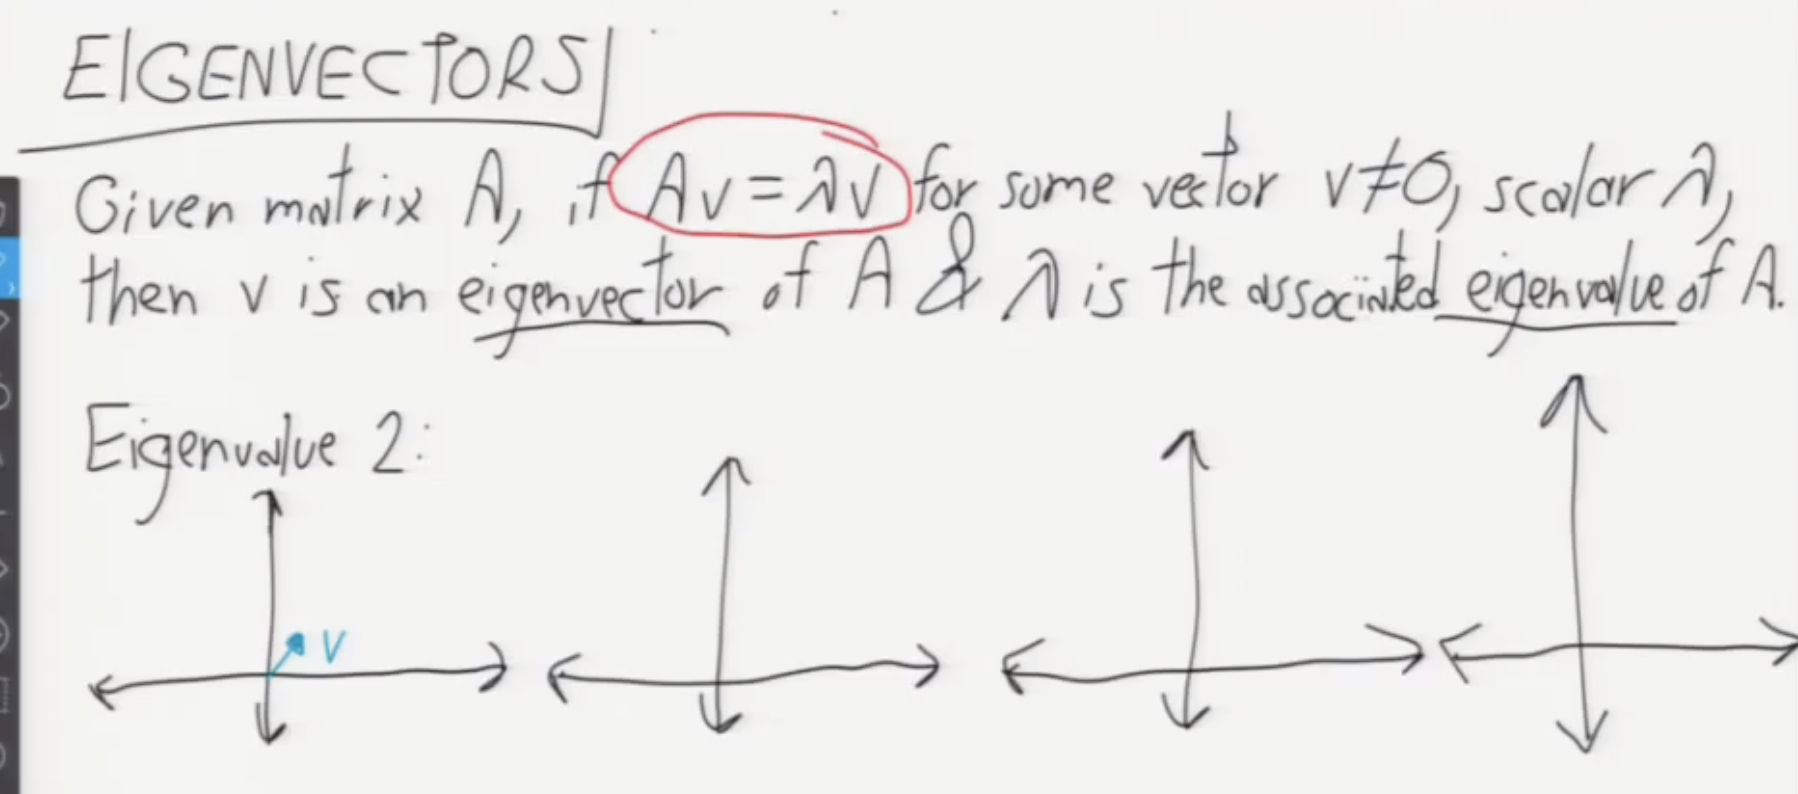
\includegraphics[width=1.0\linewidth]{images/chpt08-01}
\caption{Eigenvector-01}
\label{fig:chpt08-01}
\end{figure}

So if I take that vector $v$ and I multiply it by $A$, since its eigenvalue is 2, I get another eigenvector $v$ that is twice as long and points in the same direction.

\begin{figure}[ht]
\centering
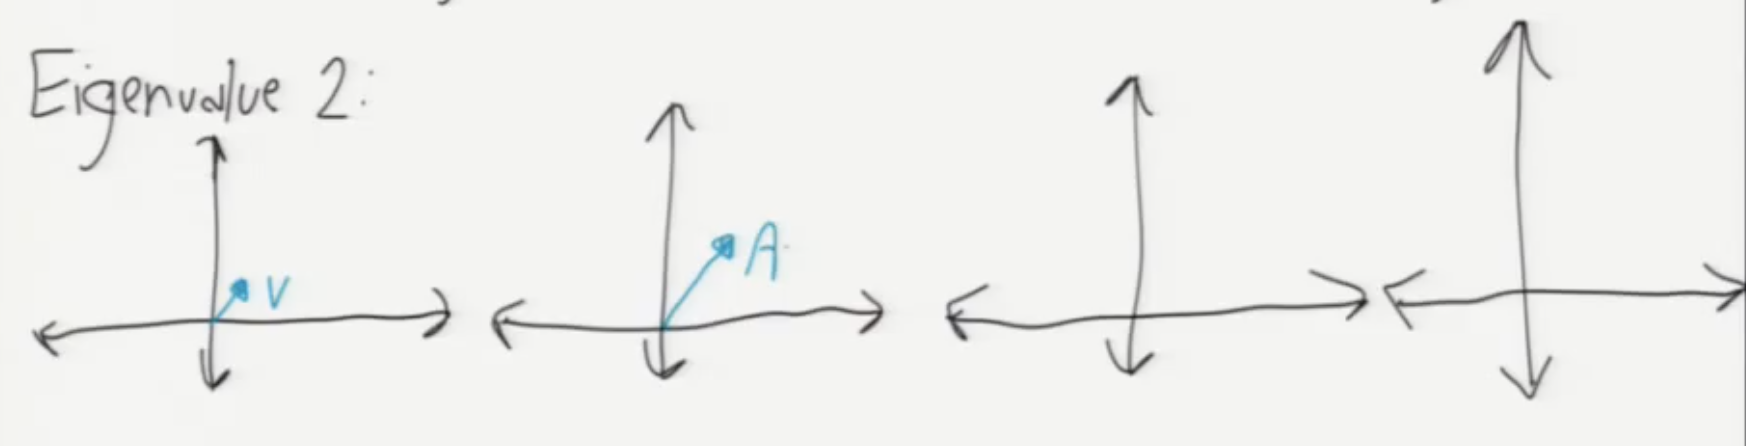
\includegraphics[width=1.0\linewidth]{images/chpt08-02}
\caption{Eigenvector-02}
\label{fig:chpt08-02}
\end{figure}
\clearpage

And we can do that again, so if I multiply it by $A$ again, so I get an vector that's twice as long, so I get another vector that points at the same direction. So now it's $A^2v$:

\begin{figure}[ht]
\centering
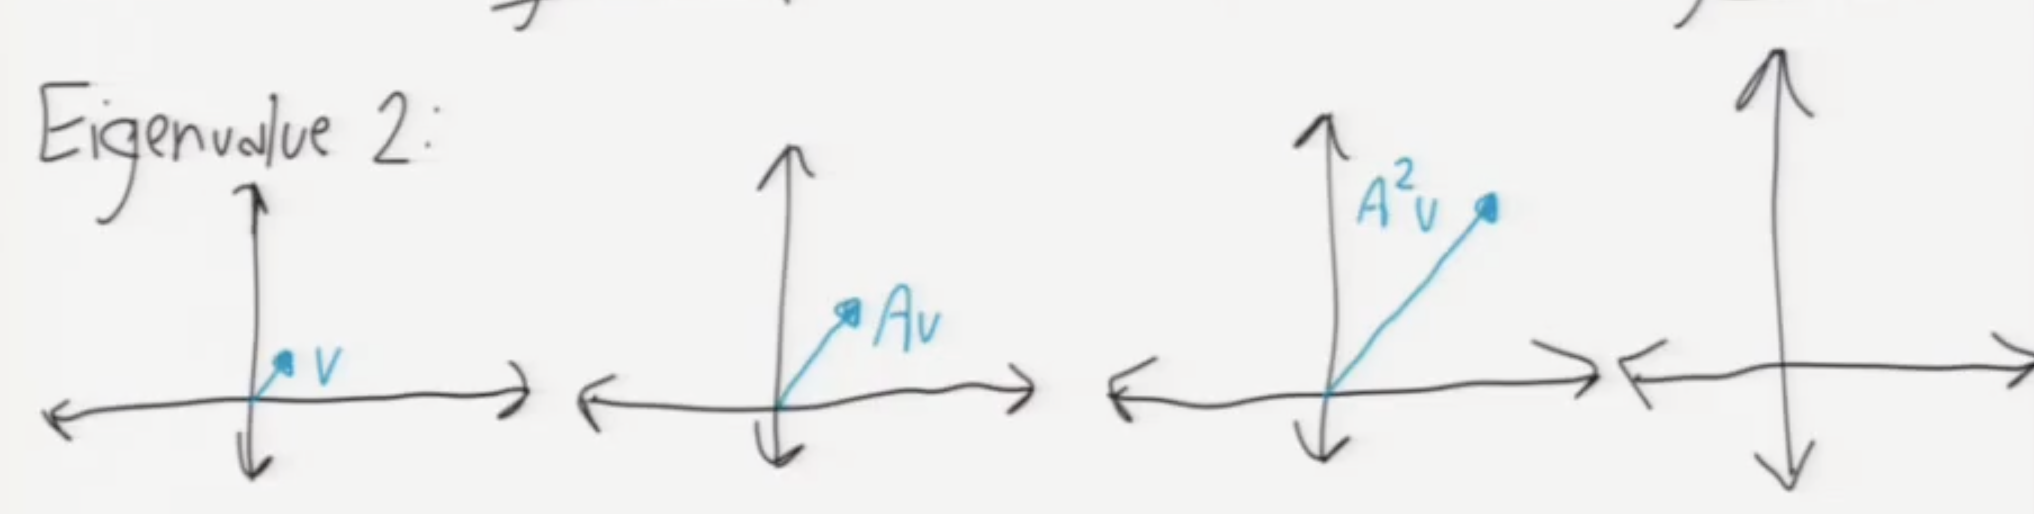
\includegraphics[width=1.0\linewidth]{images/chpt08-03}
\caption{Eigenvector-03}
\label{fig:chpt08-03}
\end{figure}

And it I do it again, I get another vector that's twice as long, and points in the same direction:

\begin{figure}[ht]
\centering
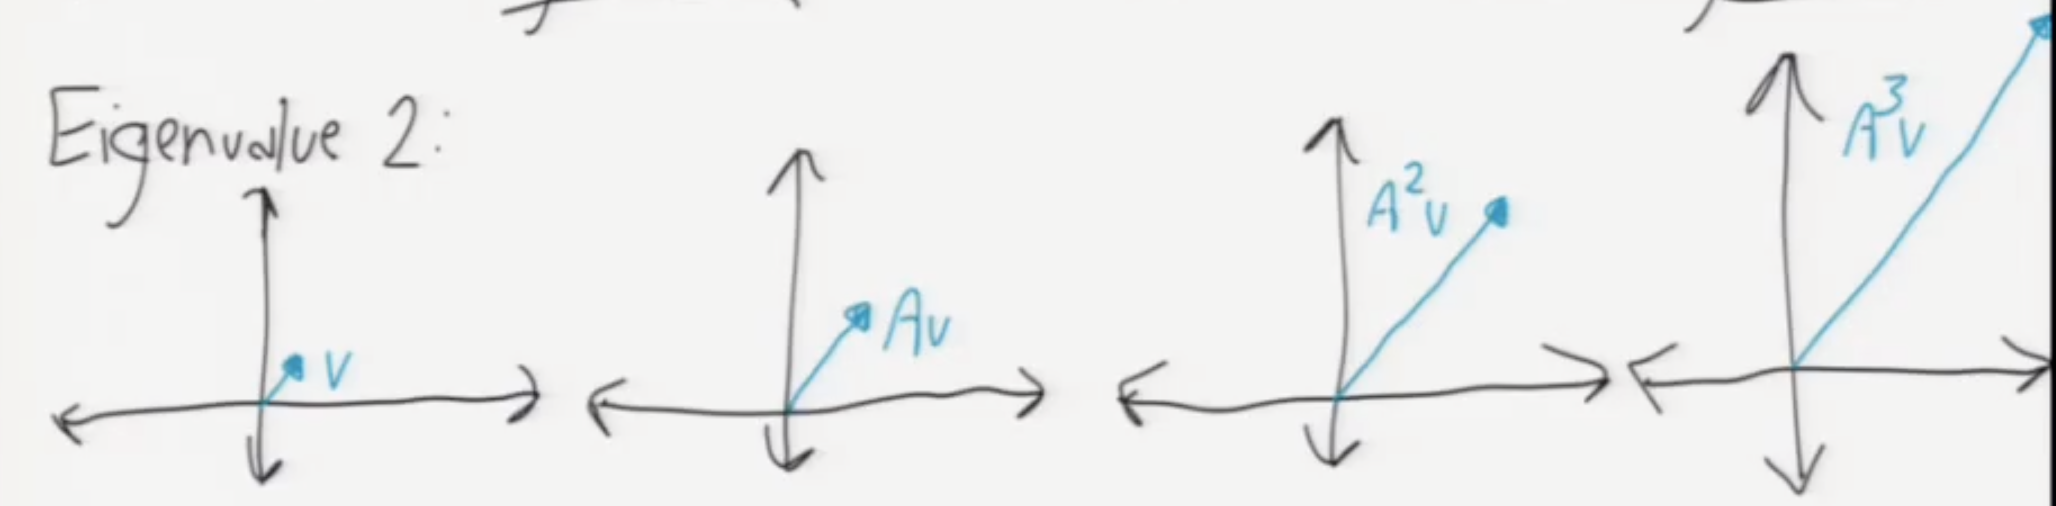
\includegraphics[width=1.0\linewidth]{images/chpt08-04}
\caption{Eigenvector-04}
\label{fig:chpt08-04}
\end{figure}

Obviously you can do this as many times as you want. And as an counterpoint, you can consider another example, where the eigenvalue is $-\frac{1}{2}$, cause we can see a few more things that's going on here. One thing is what an negative eigenvalue do and the other being what an eigenvector less that one do. Now let's suppose I got this vector here, which I'll call $w$, and let's say $w$ is an eigenvector with an eigenvalue that's $-\frac{1}{2}$:

\begin{figure}[ht]
\centering
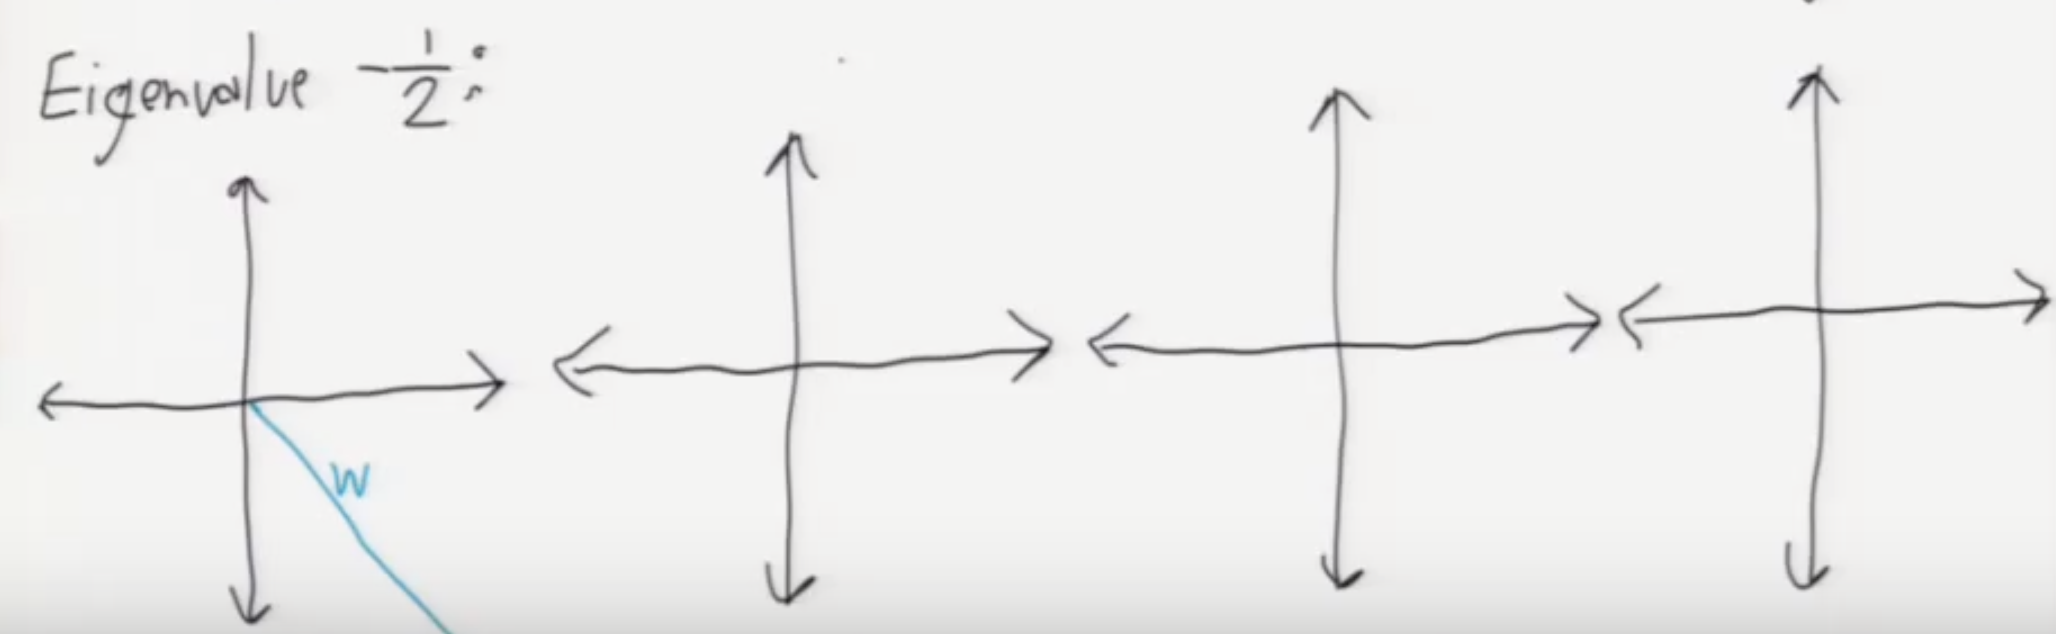
\includegraphics[width=1.0\linewidth]{images/chpt08-05}
\caption{Eigenvector-05}
\label{fig:chpt08-05}
\end{figure}
\clearpage

So if I multiply it by $A$, I get an vector that's sort of pointing at the opposite direction and only half as long ($Aw$): 

\begin{figure}[ht]
\centering
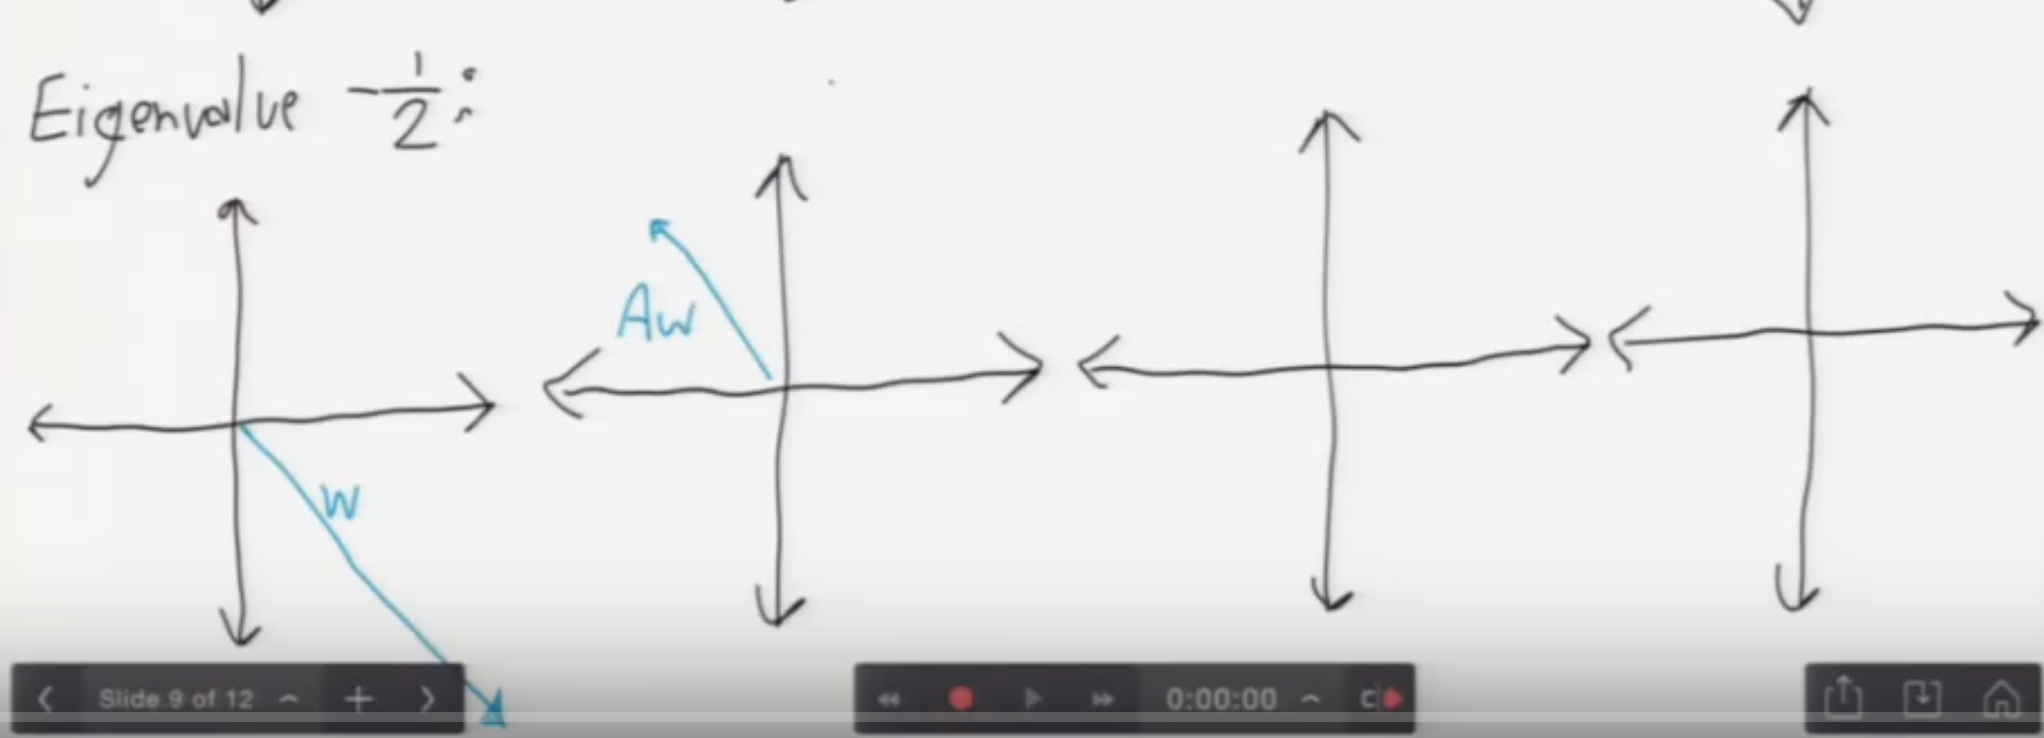
\includegraphics[width=1.0\linewidth]{images/chpt08-06}
\caption{Eigenvector-06}
\label{fig:chpt08-06}
\end{figure}

And if I do it again, I get another vector that's only half as long and pointing at the opposite direction ($A^2w$):

\begin{figure}[ht]
\centering
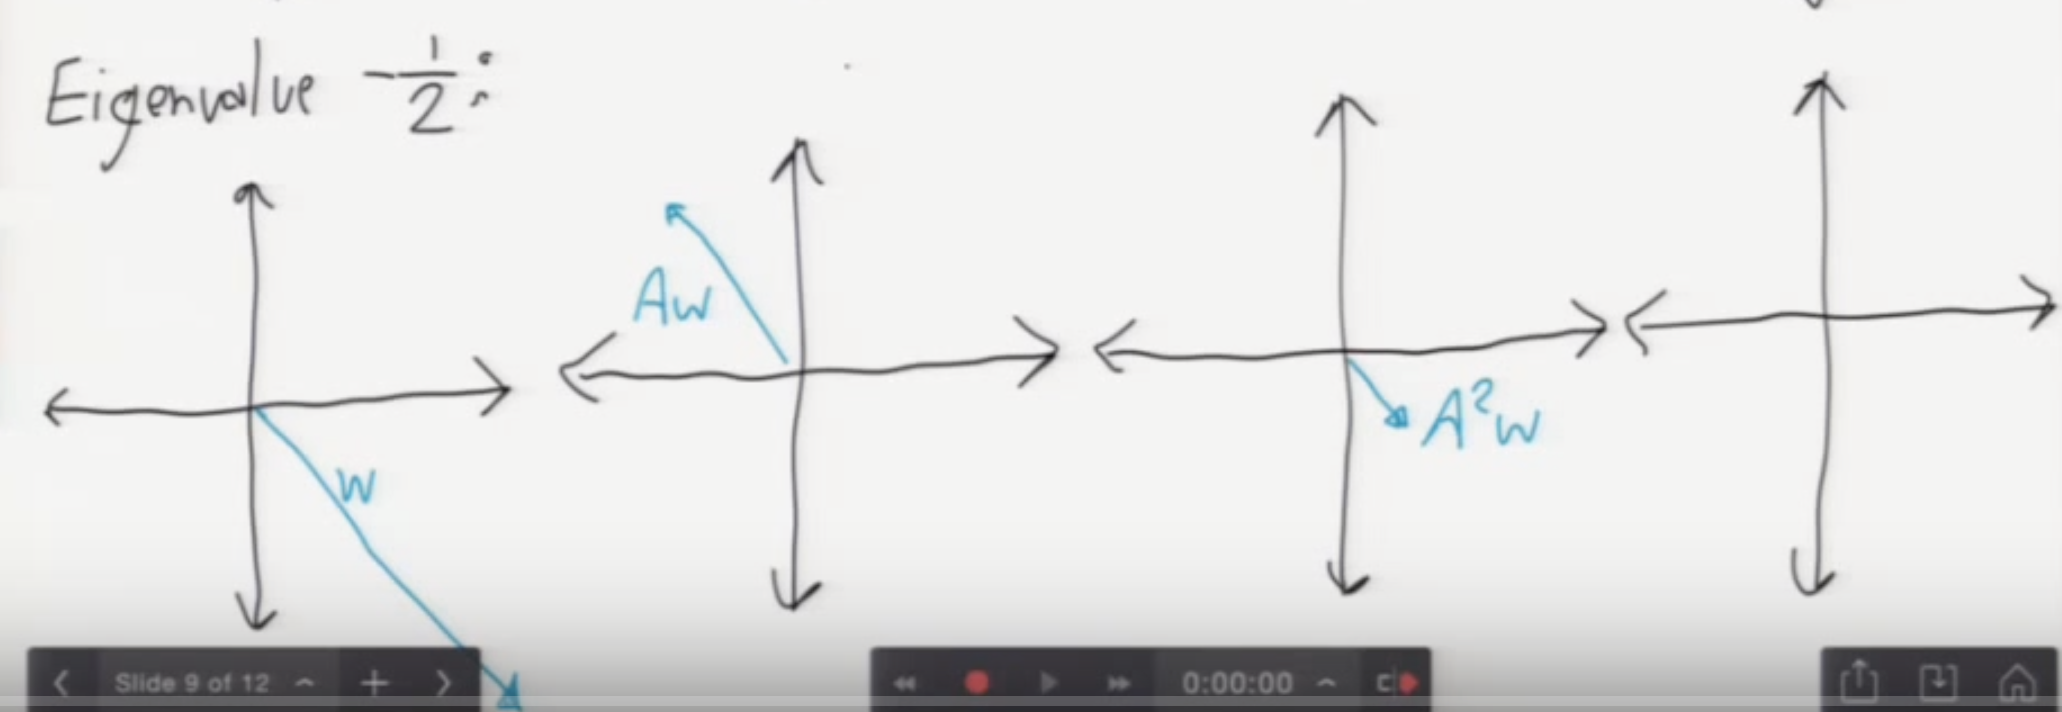
\includegraphics[width=1.0\linewidth]{images/chpt08-07}
\caption{Eigenvector-07}
\label{fig:chpt08-07}
\end{figure}
\clearpage

And I can do it again to get an even shorter vector and in the opposite direction ($A^3w$):

\begin{figure}[ht]
\centering
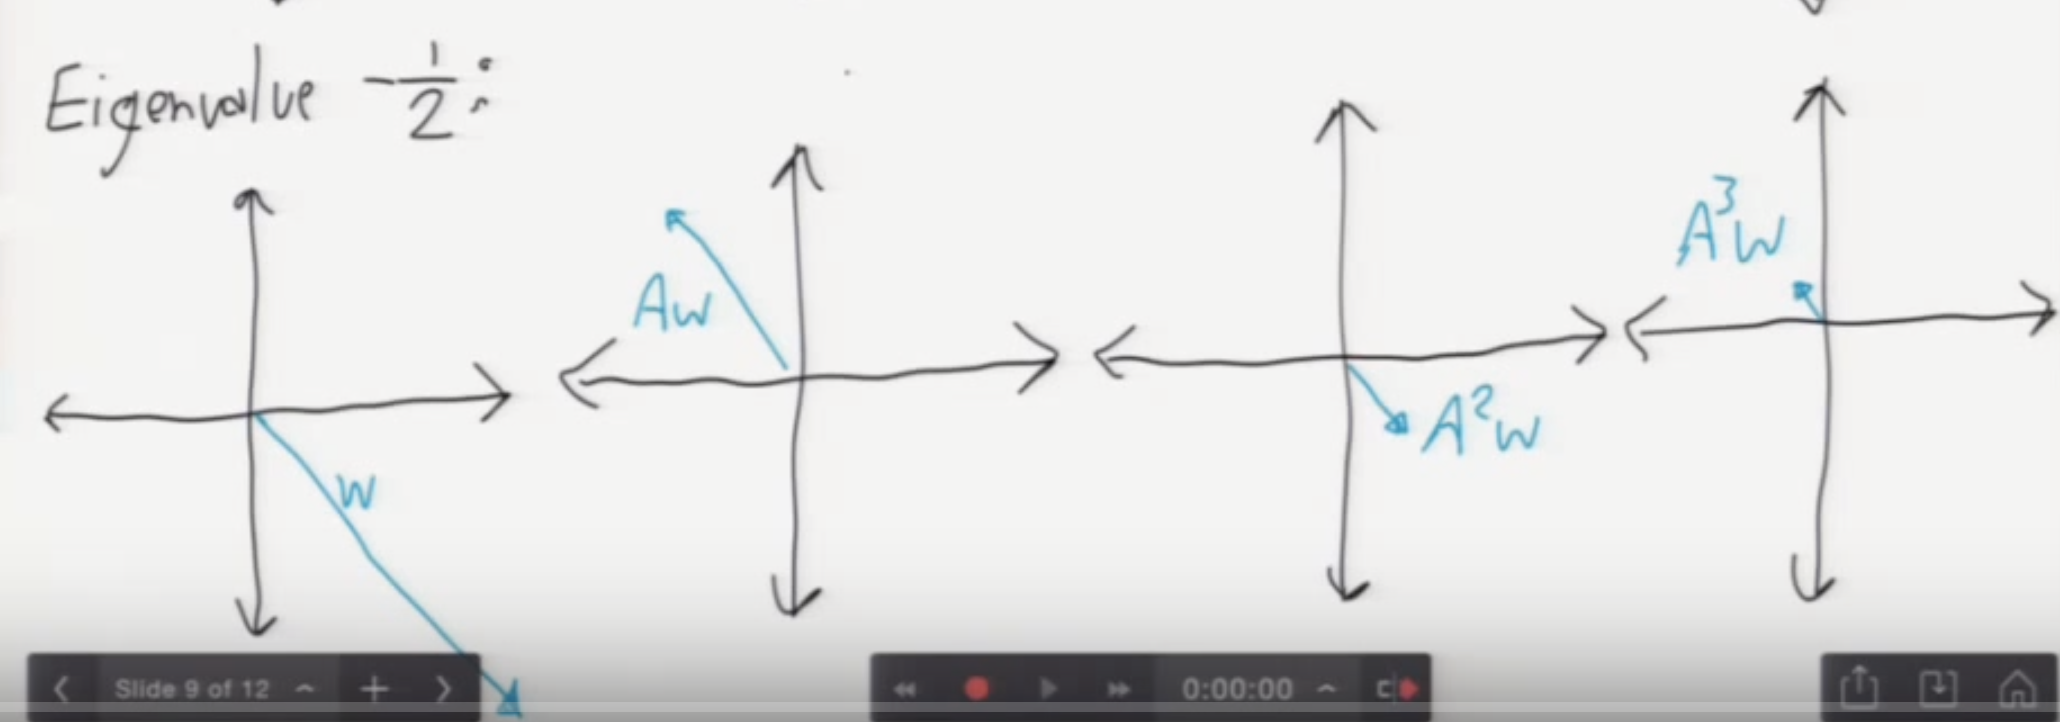
\includegraphics[width=1.0\linewidth]{images/chpt08-08}
\caption{Eigenvector-08}
\label{fig:chpt08-08}
\end{figure}

Now for most matrices, most vectors do not have this special property, so they are not eigenvectors. Eigenvectors in vectors are special and rare. And it's clear to show if an vector is an eigenvector, when you scale it, it's still an eigenvector. So when we talk about eigenvectors we only care about their directions. We usually generally don't care too much about the length. That's not implicit in the definition of the eigenvector.

So let's look at a few consequences of this fact:\medskip

\begin{theorem}
If $v$ is an eigenvector of $A$ w/eigenvector $\lambda$, then $v$ is an eigenvector of $A^k$ w/eigenvalue $\lambda^k$.
\end{theorem}

\begin{proof}
$A^2v = A(\lambda v) = \lambda^2v$, etc. (Induction)
\end{proof}

And the same thing works for matrix inversion:\medskip

\begin{theorem}
Moreover, if $A$ is invertible, then $v$ is an eigenvector of $A^{-1}$ w/eigenvalue $\frac{1}{\lambda}$.
\end{theorem}

\begin{proof}
$$
\begin{aligned}
A^{-1}v
& = (\frac{1}{\lambda})(A^{-1})(A)v \quad (\because v = \frac{A}{\lambda}v) \\
& = \frac{1}{\lambda}v
\end{aligned}
$$
\end{proof}

There's an interesting thing coming out of these two theorems, which is that I do these things to matrices, I square them, I cubed them, I invert them, the eigenvectors don't change. The eigenvalues change, they get squared, they get cubed, they get inverted, but not the eigenvectors. This is really handy.

Another interesting way to look at the last theorem is to look at the previous diagrams from right to left instead of left to right: I apply $A^{-1}$ from the fourth vector I get the third, I apply it again and I get the second.

The following theorem will be very useful in understanding the effect of an symmetric matrix on a vector that is not an eigenvector. I think you all are familiar with what's called the Spectrum Theorem, which applies only to symmetric matrices:\medskip

\begin{theorem}
\textbf\underline{{Spectrum Theorem:}} Every symmetric $n$ x $n$ matrix has $n$ eigenvectors that are mutually orthogonal: $v_i^T v_j = 0 \quad \forall i \neq j$.
\end{theorem}

This is great, this means they can form a coordinate system. The proof for the Spectrum Theorem could take up a whole page so I'm not gonna do it here. 

One minor detail I should mention is that you can have situations, for instance, where a symmetric matrix has two different eigenvectors with the same eigenvalue. When that happens, every linear combination of those two eigenvectors is also an eigenvector with the same eigenvalue. So you wind up with a matrix that has infinite number of eigenvectors, we don't want them all though, those two eigenvectors, they span a plane, all of the eigenvectors that go with them span that same plane. We just need to pick two eigenvectors in that plane that are mutually orthogonal to each other, and that's what we do in practice, cause that's what's useful.

By contrast, for any matrix, its eigenvalues are uniquely defined, the eigenvectors aren't always uniquely defined, sometimes you have to pick and choose, the eigenvalues are always uniquely defined for any matrix, including the multiplicity of the eigenvalues, some eigenvalues may appear more than once. Anyway, the upshot of the Spectrum Theorem is that \textbf{when you are dealing with a symmetric matrix, you can use its eigenvalues as a basis for space}. So now I ask what happens to an vector that is not an eigenvector when you apply an symmetric matrix $A$ to it?

When we wanna understand the effect of an symmetric matrix on an ordinary vector that is not an eigenvector, the way we do it is we break it up into a linear combination of eigenvectors. 

Recall the two eigenvectors we looked at in previous diagrams, and what I'm drawing here is another vector that's a linear combination of those two and call it the vector $x$ ($x = v + w$):

\begin{figure}[ht]
\centering
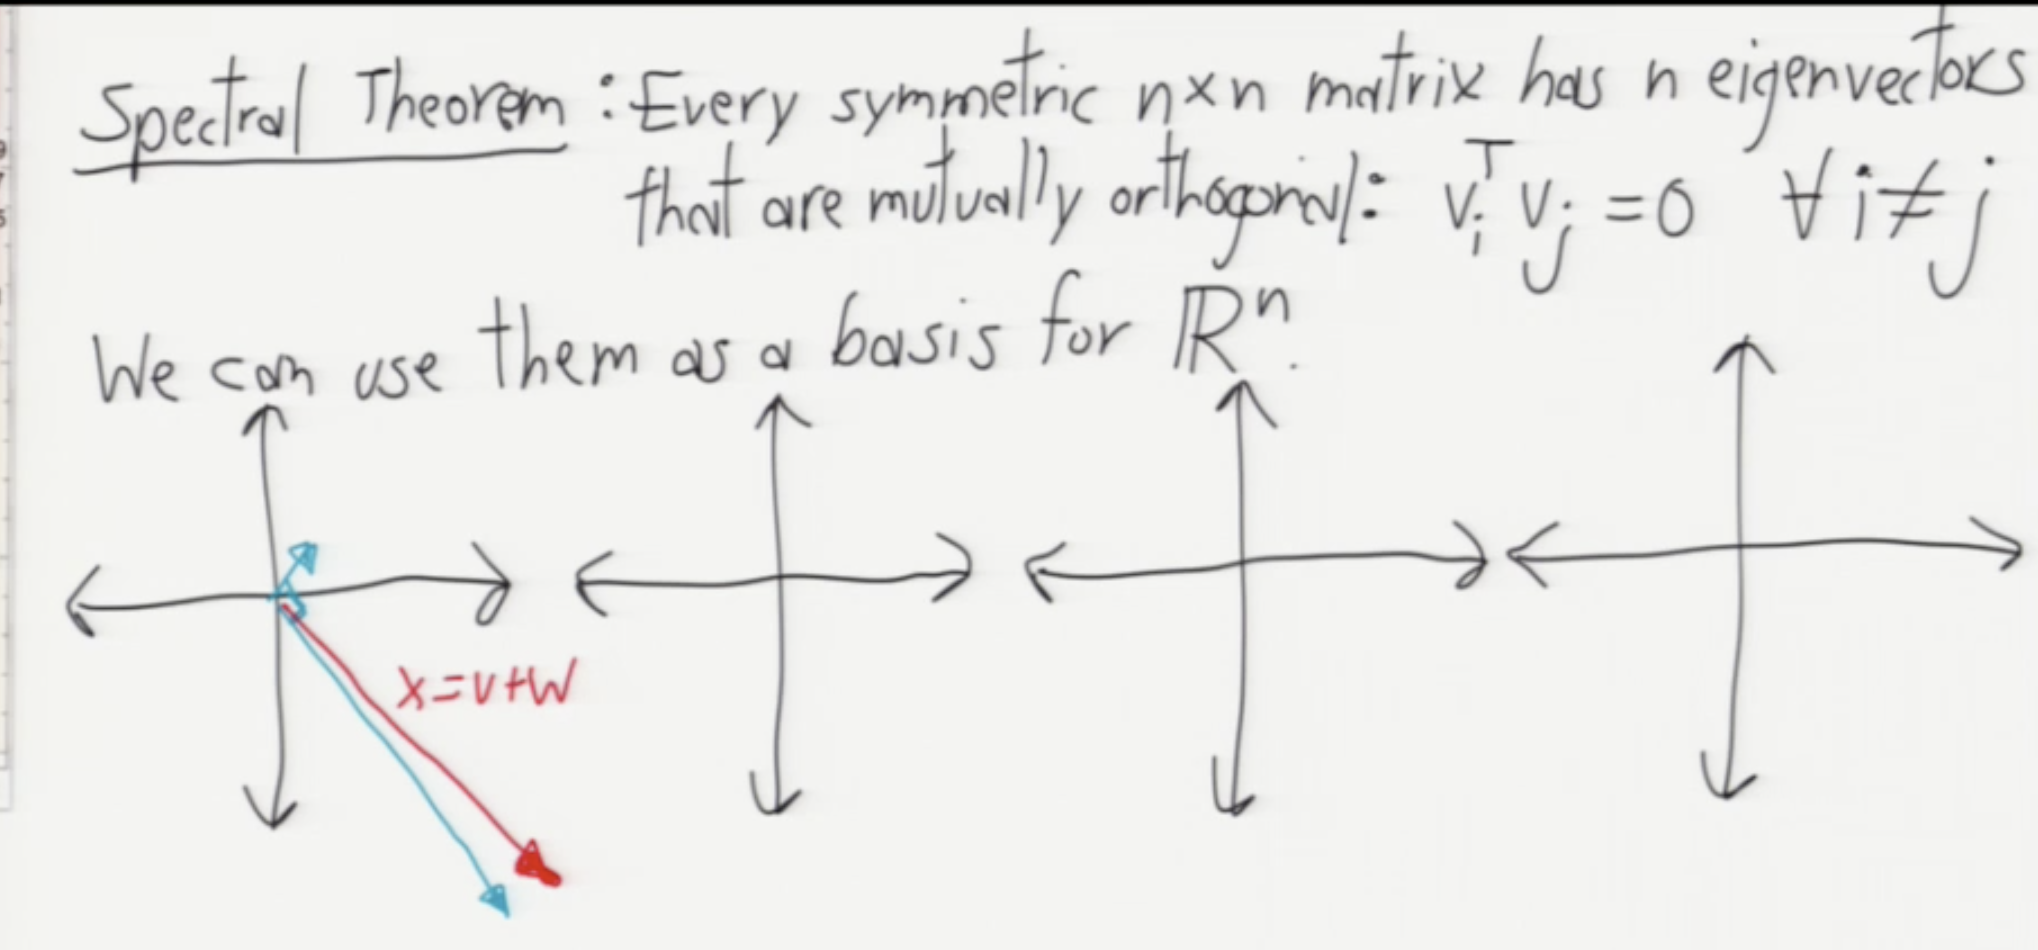
\includegraphics[width=1.0\linewidth]{images/chpt08-09}
\caption{Eigenvector-09}
\label{fig:chpt08-09}
\end{figure}

So what happens when I apply the matrix $A$ to this vector $x$? Well, I decompose it into those two eigenvectors, I look at what $A$ does to each of the two eigenvectors and then I add it up. We've already seen what happens to those eigenvectors when I apply $A$:
\clearpage

One of them is doubled. 
\begin{figure}[ht]
\centering
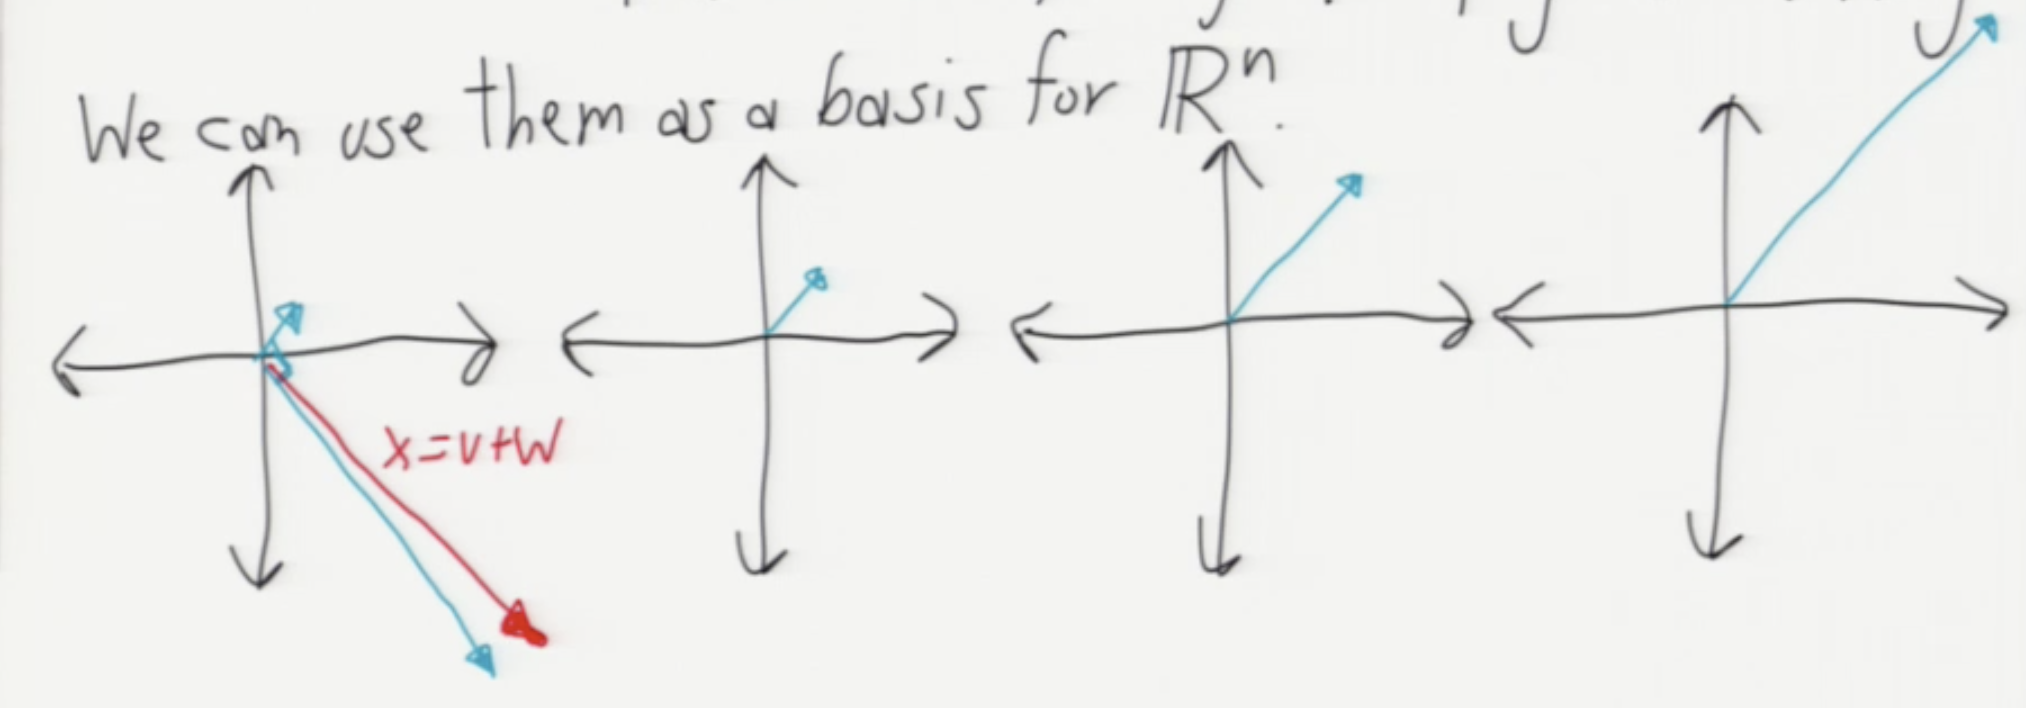
\includegraphics[width=1.0\linewidth]{images/chpt08-10}
\caption{Eigenvector-10}
\label{fig:chpt08-10}
\end{figure}

The other one kinda gets half in length and flops back and forth like a dying fish.

\begin{figure}[ht]
\centering
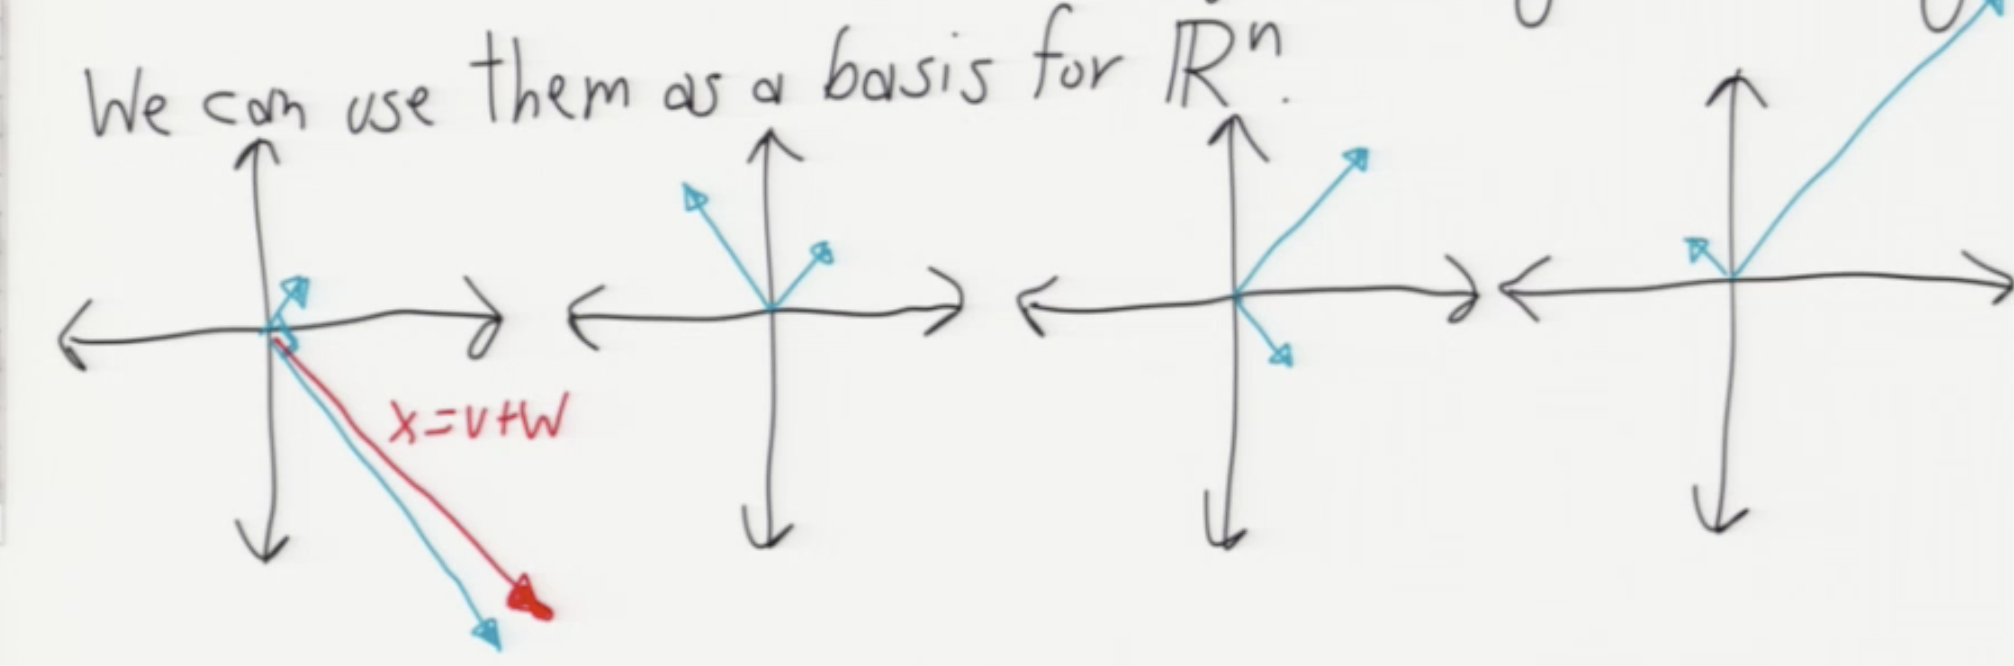
\includegraphics[width=1.0\linewidth]{images/chpt08-11}
\caption{Eigenvector-11}
\label{fig:chpt08-11}
\end{figure}

And the vector $x$, the one that we really care about, is just gonna be the sum of these two components:

\begin{figure}[ht]
\centering
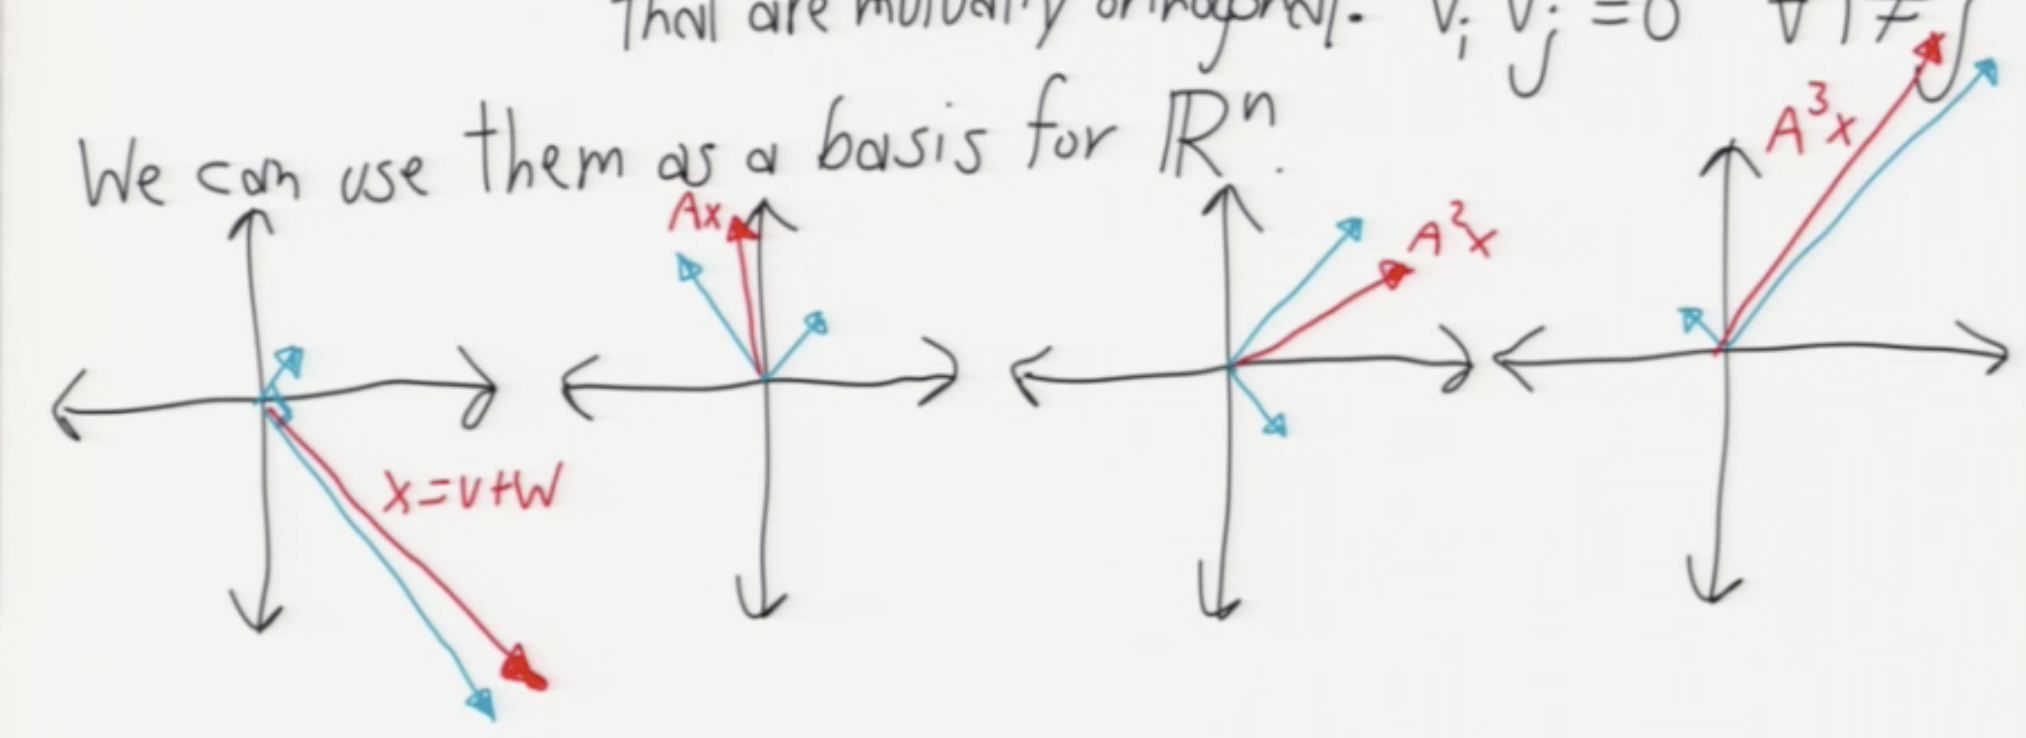
\includegraphics[width=1.0\linewidth]{images/chpt08-12}
\caption{Eigenvector-12}
\label{fig:chpt08-12}
\end{figure}

And to write down we just saw:

\begin{figure}[ht]
\centering
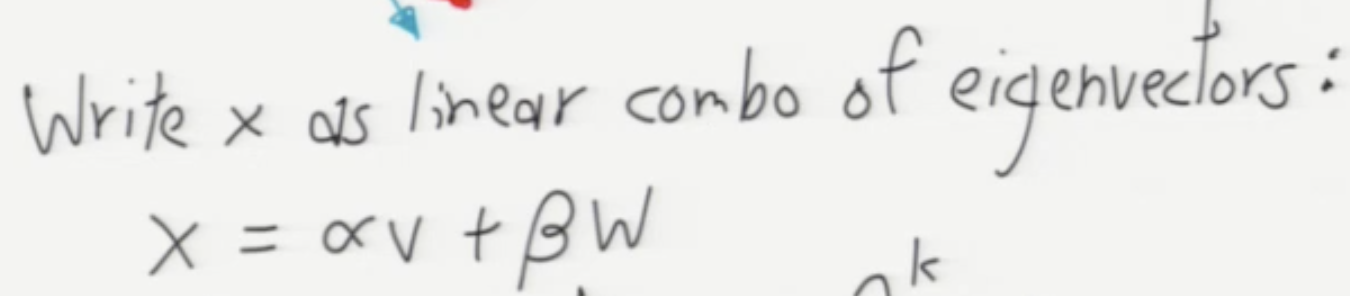
\includegraphics[width=1.0\linewidth]{images/chpt08-13}
\caption{Eigenvector-13}
\label{fig:chpt08-13}
\end{figure}
\clearpage


Remember $v$ and $w$ form a basis for a coordinate system. You can think of $\alpha$ and $\beta$ as the coordinates of $x$ in the coordinate system of the eigenvectors. So when we apply $A$ $k$ times to x, we just need to find out what effect does $A^k$ have on $v$ and $w$, and so that's what we get.

\begin{figure}[ht]
\centering
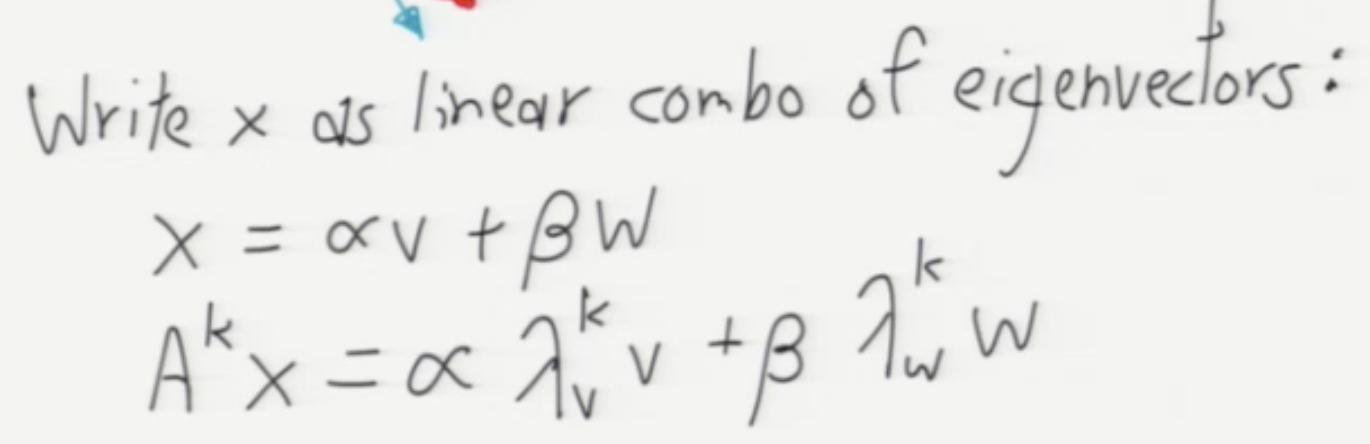
\includegraphics[width=1.0\linewidth]{images/chpt08-14}
\caption{Eigenvector-14}
\label{fig:chpt08-14}
\end{figure}



\clearpage
\section*{Machine Learning}
Machine learning is all about finding patterns from data. If you wanna describe machine learning in four words, that's probably the best I can do. And we don't just find patterns for the sake of saying "Wow, cool pattern dude", we actually use them to make predictions. See now, the reason why the NSA is going through all of your credit receipts right now is because they want to know if you're going to bomb this classroom tomorrow, and this is how you predict it. 

Now, kinda a big part of the core of machine learning is models and statistics, which are the things that help us understand patterns. Models tend to be a vague word, but it has a very specific in machine learning, which I'll try to flash our normally in a few lectures. So, a model does not mean it's how things look like. Data, if they are totally random, has no structure, but the data we're gonna look at in the real world almost always has some structure, almost always has some sort of smoothness to it. If it didn't, it wouldn't be predictable and there'll nothing for us to do. But, the question is, what is the structure of that smoothness, what do I mean when I say it's smooth or that it's regular, there're many different ways that real-world data can exhibit smoothness or regularity. And a model is a particular way your data exhibits smoothness or regularity. It's a lot easier though once you have examples of models, so take a few classes of what models usually mean. But, what you do is you sub out a bunch of models and say I believe the thing I'm trying to model is a smooth quadratic curve, for instance, or close enough to a quadratic curve with a little noise thrown in. And then, you use statistics to try to backward guess what is the most likely smooth curve that would be responsible for the data that you see. 

And the way we select a particular pattern that fits the model that we have is usually through techniques such as numerical optimization. And so we have numerical optimization algorithms that could learn the patterns, most commonly.

So one thing to understand machine learning is that we change by the exposure of data, the data is super important, the data is the most important part in machine learning. The data drives everything else. You cannot learn much if you don't have enough data. You can guess things about the world, you usually guess wrong. And also, if you have lots of data, but your data sucks because it's really noisy, or it's just wrong for some reason, like systematic errors, then you can't learn much. but, if you have lots of and lots of and lots of good data, it's amazing what you can learn, and part of what's been changing machine learning and making it a very exciting field in the last few years is that suddenly with the Internet we have huge streams of data at our finger tips. So you can go download millions of photographs, you can download a million of parrots, if you want, and there're now people who are creating 3D street views of Paris, just by assembling millions and millions of photographs together that they found on the Internet and using them, when you have enough data, you can make a very accurate model of all kinds of things. 

Another thing I should mention is that there were some machine learning techniques that have gone in and out of style, and probably the most important one is neural nets. Neural nets have gone through three phases of great popularity, separated by two phases where they were just ignored, and now we're in the third phase of great neural net popularity, specifically because we've discovered that if you have really really large datasets, and you pound those datasets with fast compute servers and parallel cloud distributors that we are computing, you can do amazing and amazing things that you couldn't do before. 

So, I want to look at an example of a machine learning task. This particular task obtained a lot of fame during the second wave of popularity of neural networks when a very good neural network was trained to recognition of digits, written on postal codes, for the U.S. Post Office. And, so, eventually it became a time when 15\% of the mails sent through the U.S. the post code were read by the automatic postal code readers, based on neural nets. And so the problem here is, people write digits, there's 10 digits we usually care about and we wanna distinguish them from each other. FOr the sake of discussion right now, we just simplify the task and pretend there's only two digits: 7 and 1. And so if you have a bunch of hand-written sevesn, the top row, and you have a bunch of hand-written ones, then how do you learn to distinguish them from each other?

So, the first step is collecting lots and lots of training images, there they are. Often that's the hardest of the machine learning task by the way. but we'll move on to the more interesting parts. 

So, the digits that we're given, they are pixels, in some small box. Let's pretend it's a really small box, and each of those pixels has some intensity. Right now, we're just looking at black and white images, so it'll be a grayscale intensity. ANd so, you can think of the input for one digit is looking like this:



Obviously it's gonna be bigger than four-by-four, but that's what I can draw right now. What we're gonna do with these digits is for now, this may seem like a really dumb thing to do, but we're just gonna express it as a vector, we'll be writing all the pixel values vertically. So there we go, we've take our digit, we have converted it into a big one-dimensional array of one-numbers. And when we do that, we think of that grid of digits as a point in 16-dimensional space. So, as a general rule in machine learning, you have some data, you take that data, and you imagine it to be some point in high-dimensional space. I know it's hard to think of high-dimensional spaces sometimes but that's what we're gonna do a lot in this class. 

So we now have a bunch of points in 16-dimensional space and you want to know is there some structure, like can we build the wall, so that all the sevens are at one side of the wall, and the ones at the other side of the wall. If we can do that, we can distinguish sevens from ones. 

So this brings us to the idea of classification, now I just got points in 16-dimensional space, I can't draw 16-dimensional space. So I'm gonna start you off with an example in an 2-dimensional space. The idea here is that instead of digits, 




















\clearpage
\section*{Neural Network}
In machine learning, what we usually deal with are two kinds of problems: classification and regression. And neural networks can do both. Neural networks tie a lot of different ideas together like perceptrons, logistic regression, ensemble of learners, and of course, stochastic gradient descent to train them. You can lift samples from a lower dimension feature-space to a higher dimensional space. But neural network has a great twist, which is they can actually learn features on their own if you can think of good ones. Maybe a neural net will find the best features for you. 

I wanna to begin by reminding you of the story I told you at the beginning of the semester, about Frank Rosenblatt’s invention of perceptrons in 1957. Remember that he held a press conference where he predicted that perceptrons would be “the embryo of an electronic computer that [the Navy] expects will be able to walk, talk, see, write, reproduce itself and be conscious of its existence. Perceptron research continued until something monumental happened in 1969. Marvin Minsky, one of the founding fathers of AI, and Seymour Papert published a book called "Perceptrons." Sounds good, right? Well, part of the book was devoted to things perceptrons can’t do. And one of those things is XOR.

If we look at our traditional exclusive OR table:

\begin{figure}[ht]
\centering
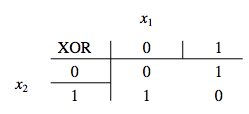
\includegraphics[width=0.3\linewidth]{images/XOR}
\caption{XOR Table}
\label{fig:XOR Table}
\end{figure}

You got two inputs $x_1$ and $x_2$, and the output, you can see them as points in a 2-dimensional space. So these aren't just numbers I'm drawing here, these are four sample points in a 2-dimensional space: two of them are of Class 0, and two of them are of Class 1. And remember perceptrons can only classify sample points that are linearly separable. 

Is this linearly separable? Can we divide it with this line?
\begin{figure}[ht]
\centering
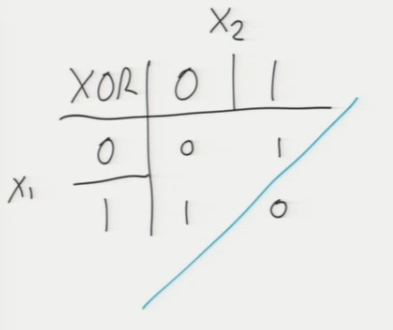
\includegraphics[width=0.25\linewidth]{images/XOR_1}
\caption{XOR Table Line 1}
\label{fig:XOR_Table_Line_1}
\end{figure}

Nope. No good. 
\begin{figure}[ht]
\centering
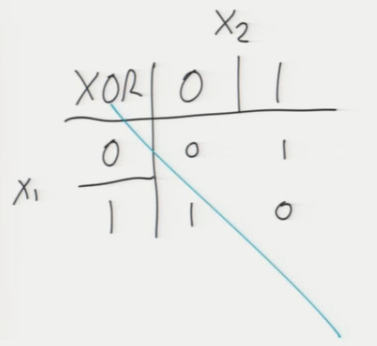
\includegraphics[width=0.25\linewidth]{images/XOR_2}
\caption{XOR Table Line 2}
\label{fig:XOR_Table_Line_2}
\end{figure}

What about this line?
\begin{figure}[ht]
\centering
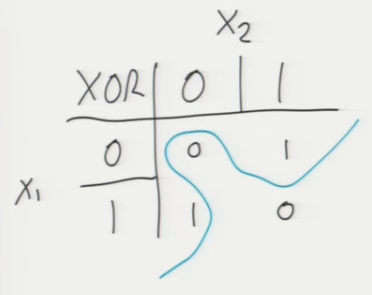
\includegraphics[width=0.25\linewidth]{images/XOR_3}
\caption{XOR Table Line 3}
\label{fig:XOR_Table_Line_3}
\end{figure}

There we go. But that's not a line. These four points are not linearly separable. So, this is one of the most basic things you can think of about logic gates, but if you can't do that, how can you convince me you can solve more complicated problems, let alone mimicking how a human think or classifying images or something like that? You are telling me this machine is gonna be conscious of its own existence but it can't do XOR? This book has a devastating effect on the field. After its publication, almost no research was done on neural nets and similar ideas for about an decade. And that's a time we now call the AI Winter. And shortly after the book was published, Frank Rosenblatt died. Officially his cause of death was a boating accident, but we all know he died of a broken heart.

Looking at this problem, one thing I can't quite understand though is why at the time why didn't some people point out some obvious ways of getting around this problem. Here's the easiest way to get around this problem: 

If you add one new feature to bring our points to a 3-dimensional space, we're gonna do a quadratic feature, the one that particularly helps in this situation is the one where you multiply the two inputs $x_1x_2$ together. And having done that, XOR is linearly separable in 3-dimensional space. And this is how it could look like:
\begin{figure}[ht]
\centering
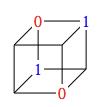
\includegraphics[width=0.15\linewidth]{images/XOR_cube}
\caption{XOR Cube}
\label{fig:XOR_Cube}
\end{figure}

So that's one way to solve the XOR problem, but there's an even more powerful way to do XOR which is what led us to the idea of neural nets. And the idea is:
\begin{description}
\centering
\item[\textit{Idea:}]\textit{ let's design some classifiers who outputs are inputs for other linear classifiers.}
\end{description}
\vfill

Let's picture the perceptrons are like this. 
\begin{figure}[ht]
\centering
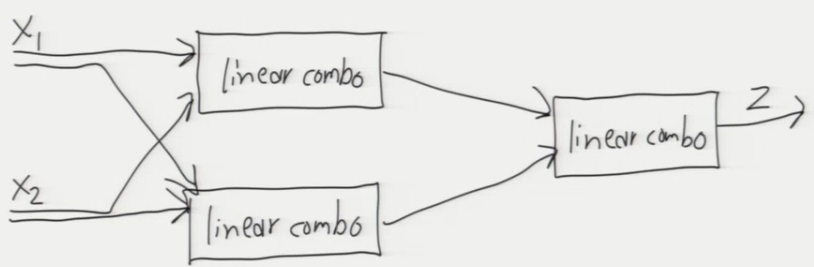
\includegraphics[width=0.75\linewidth]{images/linear_combo_boxes}
\caption{Linear Combination Boxes}
\label{fig:linear_combo_boxes}
\end{figure}

We have a box which represents a linear combination of its inputs $x_1$ and $x_2$. And then I do a second box that computes a different linear combination of the same things as inputs. And then I'll take the outputs of those and feed them into another linear combination. And there we have an output $z$. So I ask you: let's suppose that our interpret rule for the output is if $z$ is positive we're gonna call it a binary 1, if $z$ is negative, we're gonna call it a binary 0. So can we do XOR with this setup?

No, because it's the same thing as before. There's a problem here, which is that a linear combination of a bunch of linear combinations is just a linear combination of the original inputs. And so that means this cannot work for XOR, because it can only work for things that are linearly separable. And XOR is not linearly separable. 

So yeah, this doesn't work. But, fortunately, this idea is really close to something that CAN work. We need one more idea to make neural nets work. And the idea is we have add some sort of non-linearity between first two boxes and third box on the right. And by putting the right kind of non-linearity, we break this "a linear combo of other linear combos" and this allows us to start doing more interesting things that are not linearly separable. And in fact, they can get arbitrarily complicated because a little non-linearity in the middle is gonna allow us to build arbitrarily boolean circuits, for instance.
\begin{figure}[ht]
\centering
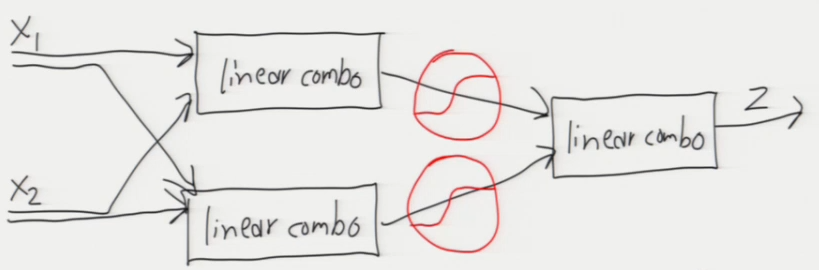
\includegraphics[width=0.75\linewidth]{images/linear_combo_boxes_nonlinear}
\caption{Linear Combination Boxes with Nonlinearity}
\label{fig:linear_combo_boxes_nonlinear}
\end{figure}

So what I'm proposing is that there needs to be some sort of modifiers here that takes the input and maps it to a slightly different output before we go to the next linear combination box. And there's more than one function we can choose  to introduce that non-linearity. But by far, the most popular is the logistic function, the logistic function seems to work really well in logistic regression for classification, so why not see if it'll work well here. So what that means is the logistic function is this S-shaped function, the output always varies between 0 and 1, however big or small the input is, and that's gonna introduce the right kind of non-linearity to allow us to do very general things. 

By the way, it doesn't have to be this complicated non-linearity to work, an non-linearity is simple as clamping the output so it cannot go below zero, can work too. And in fact, it's also used in practice a lot. but we'll start with the sigmoid and move on to other possibilities later.

So, the logistic function has a couple of nice characteristics. One is that since it's always bounded between 0 and 1, it's not going to get two big and over-saturate the other boxes or neurons, as we call them, that its output is going into. So it's nice that it can't get too big, it doesn't get too over-saturate the next neuron down the line. Another nice thing about it is that it's continuous smooth differentiable, well-defined derivatives. And that's helpful because it means we can do gradient descent relatively easily. And indeed, we're gonna train these things with gradient descent. 

So if we use this logistic function, then here's how we can do XOR, with the three boxes I just drawn, but this time I'll add logistic function to make this work. And the idea is if I have inputs with column X and Y for simplicity, and I write the following linear combination, $30-20x-20y$, and then we run the output through the logistic function, that actually acts an awful lot like an NAND gate, providing the inputs $x$ and $y$ are in some reasonable range like 0 to 1. And, I'm gonna add a similar gate at the bottom, which acts like an OR gate by taking the linear combination $20x+20y-10$, and run it through the logistic function. So we take the output of those two gates and I can devise an AND gate by taking $20v+20w-30$ with the logistic function. And the output is essentially x XOR y. 
\begin{figure}[ht]
\centering
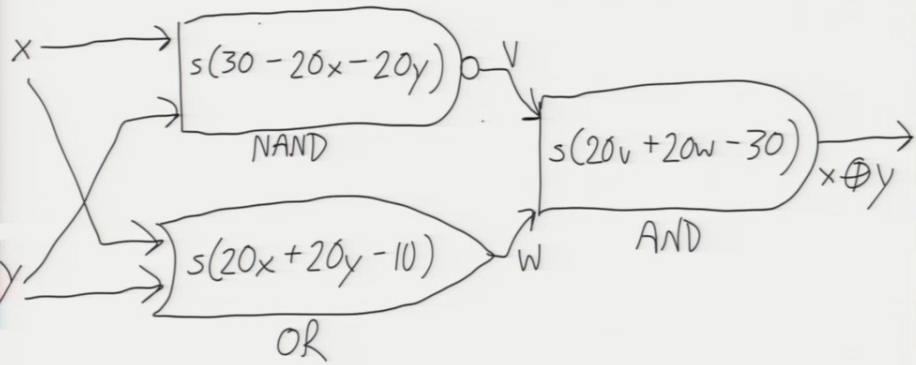
\includegraphics[width=0.75\linewidth]{images/linear_combo_boxes_nonlinear_xor}
\caption{XOR with Nonlinearity}
\label{fig:linear_combo_boxes_nonlinear_xor}
\end{figure}

Of course it's not exactly $x$ XOR $y$, because the function never outputs exactly 0 or 1, but it gets pretty close to 0 or to 1, so what we do is for a value that is lower than half, we count it as a 0 and for a value that is more than half, we count it as a 1. 

And the reason why I chose these large constants here (20, 20 and 10) is just to make sure it's large enough to drive the gate to saturation. Either the linear combination is gonna be ten or higher, or it's gonna be -10 or lower, providing the input being 0 or 1. So then once you apply the logistic function, the output is gonna be pretty close to the 0, 1. And that's how you do XOR in a neural net.

\subsection*{Network with 1 Hidden Layer}
The next thing I wanna do is setup a specific neural net and some notation that we can work with so we can start deriving algorithms and in particular, figure out how to do gradient descent. 

I'm gonna start with a neural network that has one hidden layer of neurons or units. There are three layers in total because neural nets generally have  an input layer, the $X$ you'll put into your classification algorithm, and then you'll have an output layer, which is $Y$, and sometimes we might have more than one output, so we may have more than one $Y$. 

So again, the input layer is the usual usual, we have a vector $x$ that is our input vector, and it has ${d}$ components. I'm also going to have a convention that every input vector has a hidden ${d+1}$ component, which is ${1}$, the usual fictitious dimension trick.

We're gonna have a layer of hidden units, and their outputs are gonna be ${h_1}$ through ${h_m}$ where ${m}$ is the number of hidden units, or the number of hidden neurons if you prefer. And again, we're gonna use the fictitious dimension trick as well, because we want to be able to have all linear combinations and a linear combination has a constant $1$. 

And we'll have an output layer, which I'm gonna call these $Z$s, the predicted outputs and there will be up to $k$ of those.
\begin{figure}[ht]
\centering
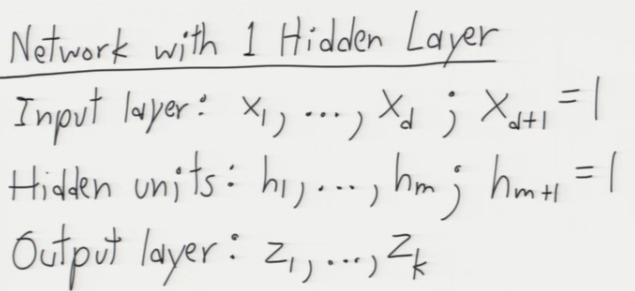
\includegraphics[width=0.7\linewidth]{images/nn_with_1_hidden_layer}
\caption{Network with 1 Hidden Layer}
\label{fig:nn_with_1_hidden_layer}
\end{figure}

Now, through out this semester we've been doing various classification algorithms. We take an $X$ in, and your output is usually just like one thing, like in classification it's one class, in regressions the output is one number. Now we're gonna sometimes have more than one output, what's special about that?

So, generally if we're using an algorithm like SVM, or logistic regression, if you want to do more than one output, that's just like doing more than one classifier. So you train every classifier separately, once for each output. With neural nets it actually makes sense for us to group outputs together and the reason why is sometimes you get unexpected benefits by having all your outputs come from the same set of hidden units, because what can happen sometimes is that a hidden unit that's being trained to support one of these outputs suddenly becomes unexpectedly useful for correctly predicting another one of the outputs, and you wind up predicting that other output better than you predicted it with just training that one output by itself. So by training outputs, sometimes you get better classifiers in some of those outputs than you training them apart because they're sharing particularly intelligent hidden units. 

We need to have a notation for the weights for those linear combinations. For layer 1 weights, We're just gonna express them as a matrix, called $V$. And the reason why it is a matrix is because every input is gonna contribute to every hidden unit. So we have a matrix that says how much of these inputs contribute to this particular hidden unit, what is the coefficient of the linear combination that links them together. And I'll use the notation $V_i$ for row $i$ of the matrix. We also have another layer of weights, I'll call it layer 2. They connect these hidden units to the output. And I'll call that matrix $W$, again $W_i$ represents the ith row of that matrix, which is important to that particular output, row i corresponds to output i. 

We'll be using the logistic function and so, let me just remind you what that is. Now again, as I said before, other non-linear functions can be used and are often used. I'll probably talk about them on Monday. 

And I want to apply $s$ not just to a scalar, but to vectors, and when I apply it to a vector, it's just applying it component by component, nothing special. So, when we have a vector $v$, and I write $s(v)$, that just means applying $s$ to each of the component of the vector. 
\begin{figure}[ht]
\centering
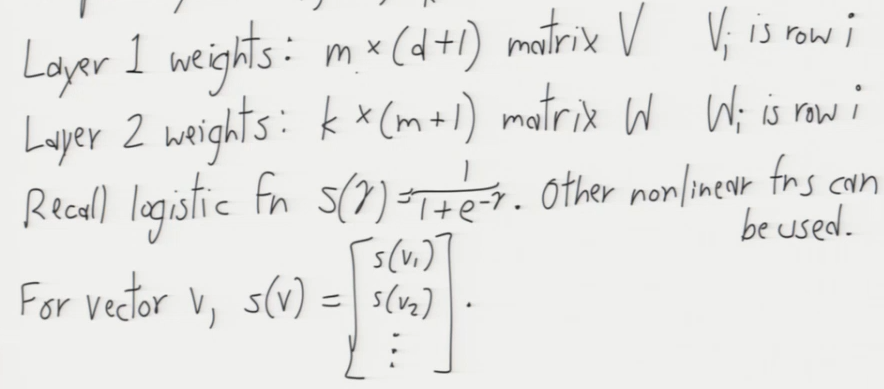
\includegraphics[width=0.7\linewidth]{images/nn_with_1_hidden_layer_notation}
\caption{Network with 1 Hidden Layer Notations}
\label{fig:nn_with_1_hidden_layer_notations}
\end{figure}

Alright, so that's the notation that we'll use. Now let me draw these things so you can see how everything relates. I'm gonna have three hidden units in the middle, I'm gonna have two input units on the left, and two output units on the right. For this particular example, of course, neural nets are usually bigger than these, but we want to keep our drawing within bounds. And every input has a connection to every hidden unit, and every hidden unit has a connection to every output. And each of these edges has one weight. These edges on the left, their weights are stored in the matrix $V$. These edges on the right, their weights are stored in the matrix $W$. So for instance, this edge here is $V_{11}$, this edge here is $V_{21}$, you put first the number of neuron it's going to and then the number of neuron it's coming from. So $V_{21}$ means we're going from $X_1$ to $h_2$, cause the matrix calculation works out right that way. Likewise, on the output layer, we'll have weights in the $W$ matrix, and they are numbered in the same way.
\clearpage

\begin{figure}[ht]
\centering
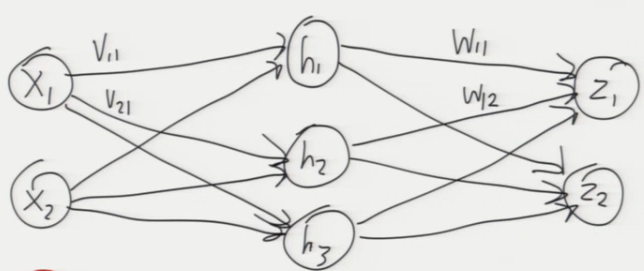
\includegraphics[width=0.7\linewidth]{images/nn_1_layer_diagram}
\caption{Network with 1 Hidden Layer}
\label{fig:nn_1_layer_diagram}
\end{figure}

I'm also including a few ghost variables that are equal to one. So, remember $X_3$ is equal to one, $h_4$ is equal to one, we want to do any linear combinations, so we need a constant term for every linear combination. So, imagine the arrows are here, you know, we won't actually have a unit per se, in your code, for these two nodes, but we do have these red edges. Those are the bias weight, the constant weights in your linear combinations. And so, they are important too. 
\begin{figure}[ht]
\centering
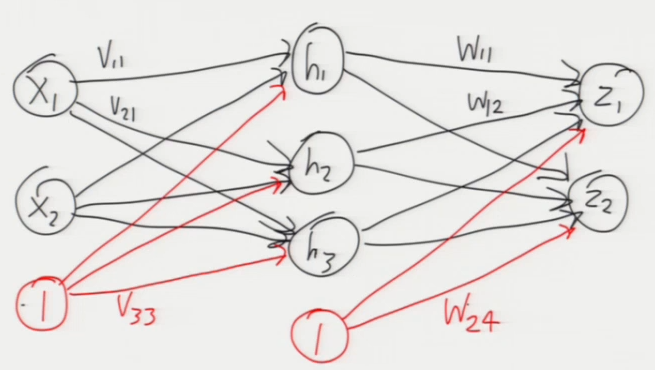
\includegraphics[width=0.7\linewidth]{images/nn_1_layer_diagram_w_bias}
\caption{Network with 1 Hidden Layer with Bias}
\label{fig:nn_1_layer_diagram_w_bias}
\end{figure}
$$\mathbf{x} = 
\begin{bmatrix}
x_1 & x_2 & ... & x_d & 1
\end{bmatrix}^T,\quad
\mathbf{h} = 
\begin{bmatrix}
h_1 & h_2 & ... & h_m & 1
\end{bmatrix}^T,\quad
\mathbf{z} = 
\begin{bmatrix}
z_1 & z_2 & ... & z_k
\end{bmatrix}^T
$$
$$
\mathbf{V} = 
\begin{bmatrix} 
V_{1,1} & V_{1,2} & ... & V_{1, d+1} \\ 
V_{2,1} & V_{2,2} & ... & V_{2,d+1} \\ 
... & ... & ... & ... \\
V_{m,1} & V_{m,2} & ... & V_{m,d+1} 
\end{bmatrix},\quad
\mathbf{W} = 
\begin{bmatrix} 
W_{1,1} & V_{1,2} & ... & V_{1, m+1} \\ 
W_{2,1} & V_{2,2} & ... & V_{2,m+1} \\ 
... & ... & ... & ... \\
W_{k,1} & V_{m,2} & ... & V_{k,m+1} 
\end{bmatrix},
$$

Now we have everything, and we can start writing the formula here:

So, for each hidden unit, that's gonna be equal to the logistic function applied to the linear combination. So we sum over all of these input edges, the weight of that edge gimes the input value:
$$h_i = s(\sum_{j=1}^3 V_{ij}x_j)$$

And of course, we can write them shorter using the matrix notation:
$$h = s(V \cdot x)$$

So $h$ is equal to applying the logistic function $s$ to every component of the vector $V \cdot x$. 

And we do the same thing to compute $z$ from the hidden units $h$. 
$$z = s(W \cdot h)$$

$z$ is gonna be applying s to $W$ multiplied by $h$, so... weight matrix times hidden unit vector and then you apply the logistic function, component by component, to this vector $W \cdot h$.

And if you want to write this in composition, you can write the outputs in terms of the inputs:
$$z = s(W \cdot h) = s(W \cdot s_1(V\cdot x))$$

Here, I write $s_1$ just to remind myself to add 1 to the end of the vector ${V \cdot x}$ so before we can do the next matrix multiplication. 

\subsection*{Training: Gradient Descent}
Now, what we want to do is to train them, and we'll train them using gradient descent. I would say that using stochastic gradient descent, meaning one sample point at a time is the most common way to train them. But, batch gradient descent exists too. 

In order to train, we first always have to decide on what is the function we want to optimize, so we need to pick a \textbf{loss function}, $L(z, y)$, 
where $z$ is the neural net's vector of predictions, that's the output. And the $y$ vector, is the true values of what we really want to fit. Note that $y$ can be a vector or scalar. 

For now, we'll just use the square error as the loss function:
$$L(z, y)= |z-y|^2$$

Remember this is an interchangeable part of a neural net. you can swap this out and swap in some other loss function pretty easily. Once you have a loss function, then you need a \textbf{cost function} that looks not just up one input $x$, but all of the training samples. So for the cost function, we're just gonna use the simplest thing that we usually do, which is we're gonna take the sum over all of the training points of the loss function. Therefore, the cost function is
$$J(h) = \sum_{i=1}^n L(h(X_i), Y_i)$$

I'm using capital $Y$ because I'm now assuming there's an input matrix Y that has one row for each sample point and one column for each output of the neural net, i.e., assuming we have $n$ samples, 
$$
\mathbf{Y} = 
\begin{bmatrix} 
Y_{1,1} & Y_{1,2} & ... & Y_{1,d} \\
Y_{2,1} & Y_{2,2} & ... & Y_{2,d} \\
... & ... & ... & ... \\
Y_{n,1} & Y_{n,2} & ... & Y_{n,d}
\end{bmatrix}
$$
Up till now, we always use a vector $y$ because we only have one output, now we can have more than one input, so let's use a matrix. 

Now, one of the big differences between neural nets and logistic regressions, even though neural nets look a lot like logistic regressions, is that there's no longer just one local minimum. When you do logistic regression, we have a \textbf{convex cost function}, which is great, because that means there's only one minimum, which is also the global minimum, once we're there we're happy. Neural nets are like the opposite of that, there's probably billions and billions of local minima when you do a really large training set with a large network. And there's no guarantee that you're gonna find the best one, you can just hope you can find a good one. And part of the complications we're gonna deal with is how do you find a good one, but right now, let's just worry about how to find a local minimum at all. 

Let's suppose we have this \textbf{cost function}, and we wanna do \textbf{gradient descent}, and so we start with all the weights set to zero, and we start doing gradient descent on this cost function. What is going to go wrong?

Looking at the diagram of the neural net, if you set all these weights to zero, there is a symmetry between these weights in that what is the difference between $x_1$ and $x_2$, what is the difference between $h_1$ and $h_2$ and $h_3$, why should anyone of those weights come out differently than any of the other weights? What's gonna happen is if all those weights start the same, then the direction of steepest descent is going to try to change them all by exactly the same amount, and they're always gonna stay the same. You have a symmetry wrecking problem here. You have to make different hidden units, focus on different parts of the problem, and the way we do that is pretty trivial, we just start with random weights rather than starting with zero weights, and so far that seems to be working reasonably well in practice. 

Alright, just to write down the gradient descent algorithm, it's pretty simple.
\begin{figure}[ht]
\centering
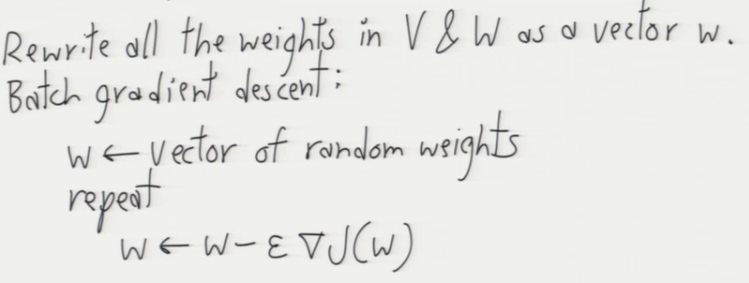
\includegraphics[width=0.7\linewidth]{images/gradient_descent}
\caption{Gradient Descent Algorithm}
\label{fig:gradient_descent}
\end{figure}

\begin{itemize}
\item Let's remember, we are storing these weights in two matrices, $V$ and $W$, so let's rewrite those as a vector, $w$. Then we do batch gradient descent in the usual manner.
\item we will start with $w$ being a vector of random weights, to break symmetry, and then we just repeat the gradient descent step.
\item Looking at $w \leftarrow w - \epsilon \triangledown J(w)$, we're descending on the whole cost function. We could do stochastic gradient descent instead, which requires us making this to be the \textbf{loss function} for one sample point. And we choose that sample point randomly or choose that sample point by shuffling all the sample points and going through in that shuffled order.
\item The important thing is that this is still the same old gradient descent algorithm you know and love, but now the weights, we think of them as being stored in two matrices, that doesn't change how gradient descent works, you just have to remember that we have to treat them as vectors in gradient descent.
\item It's important that you don't pick the random weights too big, because if the input to the neurons are big, the neurons will saturate, that means our output is very close to 1 or 0, and once a neuron is saturated, it's very hard to get it to stop being saturated. You can actually get into situations like the neurons are kinda stuck, and stuck means for every input example point, the neuron is always very close to 1 or 0. And when a neuron gets stuck like that, it's hard for it to get unstuck because the gradient is gonna be close to zero as well, so you wanna start with random weights that are not too big. 
\end{itemize}

So the hard part of this algorithm is gonna be computing the gradient $\triangledown J(w)$ here. That's actually quite tricky to do fast. It's possible to write out the formula, and if you write out the formula, what you'll find is that for any one weight, the gradient formula involves lots and lots of other neuron values and actually takes linear time to compute, linear to the number of neurons. So again, the derivative for just one weight is gonna be $O(number of neurons in the network)$. And then you'll have to do that for each weight, that means the number of neurons times the number of weights.

Fortunately, there's a clever way of getting around this, it's called \textbf{backpropagation}. Probably a lot of you have heard of the backpropagation algorithm which is kinda considered as the center of neural nets, or at least of how you train a neural net. And what that does is it gets the running time down to linear, specifically linear to the number of edges (weights), cause you have to do that to every edge at least once, to change its weight. But this is a hugely important way of making neural net practical, that you can compute the gradient in linear time instead of essentially quadratic time. It still can be quite slow, but at least it makes neural nets trainable. So we're gonna spend quite a bit of time understanding how to do this.
\begin{figure}[ht]
\centering
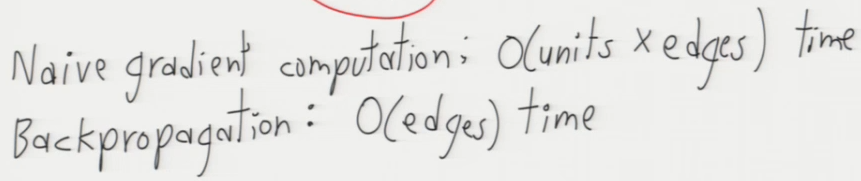
\includegraphics[width=0.5\linewidth]{images/big_o_gradient_descent}
\caption{Big O}
\label{fig:big_o_gradient_descent}
\end{figure}

\subsection*{Backpropagation}
One way to think about backpropagation is it's a glorified version of the chain rule in very large expressions. So what we're gonna do is we're gonna have to go through several phases of learning before we get to backprop. Let's start with computing gradients for an arithmetic expression.

\subsubsection*{Computing Gradients for Arithmetic Expressions}
Let's suppose we have a general arithmetic expression, and we write it out as a circuit. How do you compute a gradient for that?

And we're gonna do that by looking at the following expression: 
\begin{itemize}
\item We're gonna take the sum of numbers $a$ and $b$ and call the output $d$.
\item And the output $d$ we're gonna multiply by another number $c$
\item And then we're gonna take all of that (call it $e$) and we're gonna square it. So that output is $f$.
\end{itemize}
\begin{figure}[ht]
\centering
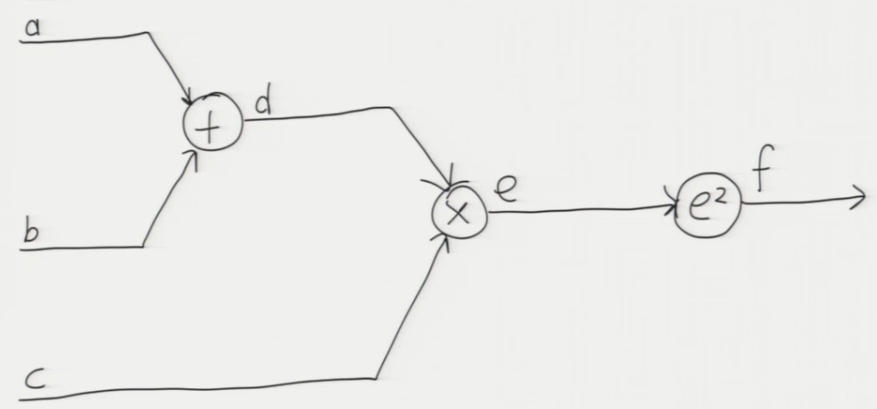
\includegraphics[width=0.5\linewidth]{images/arithmetic_expression}
\caption{Arithmetic Expressions}
\label{fig:arithmetic_expression}
\end{figure}

The goal I wanna do here is to compute the gradient of $f$. And when I say the gradient of $f$ it not with respect to all the variables here, of course we can compute all five of them, but right now the ones I really want is I want the gradient of $f$ with respect to the inputs $a$, $b$, and $c$:
$$\triangledown f = 
\begin{bmatrix}
\frac{\partial f}{\partial a} \\
\\
\frac{\partial f}{\partial b} \\
\\
\frac{\partial f}{\partial c} \\
\end{bmatrix}$$

So the question now is how do I do that?

Let's starting by going from left to right. At $a$, what we want is we want the partial derivative of $f$ w.r.t $a$. It looks kinda complicated because there're all these levels of computations between $a$ and $f$. But what I can do is I can apply the chain rule. So I can rewrite this partial derivative in terms of $a$ by throwing $d$ into the mix. 
\begin{figure}[ht]
\centering
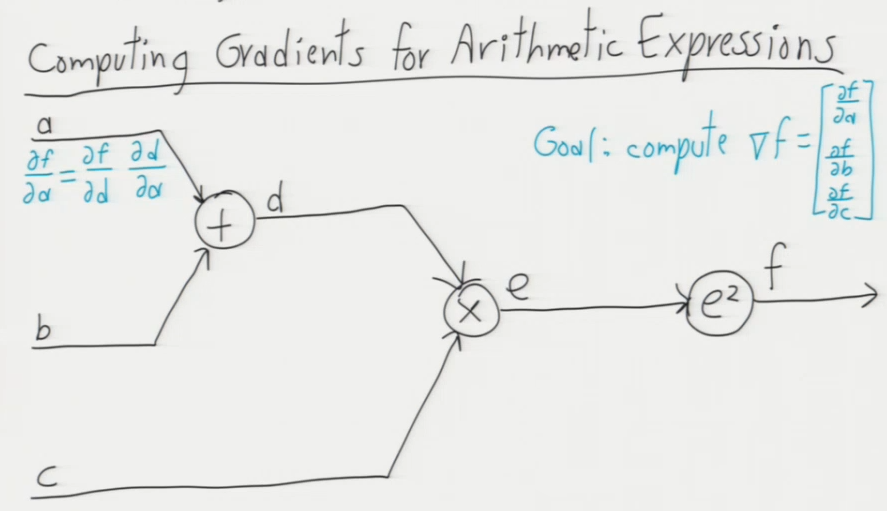
\includegraphics[width=0.7\linewidth]{images/arithmetic_expression_1}
\caption{Arithmetic Expressions}
\label{fig:arithmetic_expression_1}
\end{figure}

And I'm gonna do the same thing to the other variables here. 
\begin{figure}[ht]
\centering
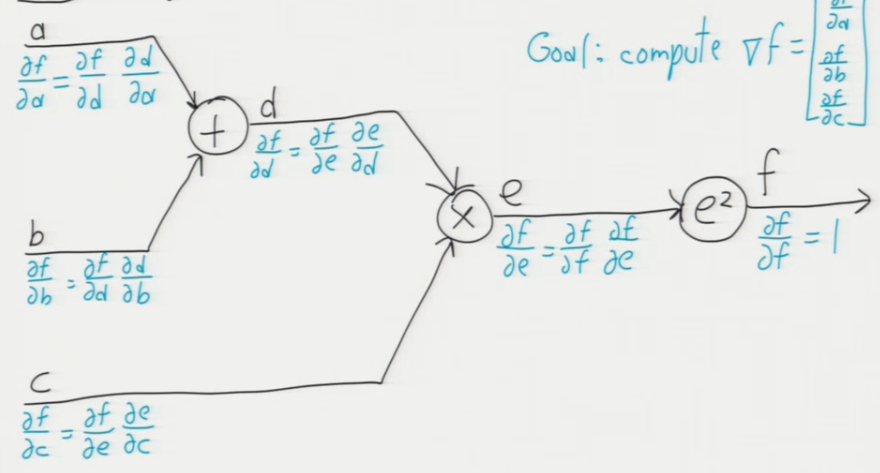
\includegraphics[width=0.8\linewidth]{images/arithmetic_expression_2}
\caption{Arithmetic Expressions}
\label{fig:arithmetic_expression_2}
\end{figure}

So now we got all these partial derivatives we need to compute. And we can compute some of them immediately as the numbers are moving forward through the circuit, but not all of them. Let's look at which ones we can compute. So, we have here $d = a + b$, and let's figure out what the partial derivatives are:
\begin{figure}[ht]
\centering
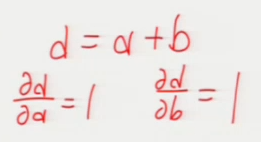
\includegraphics[width=0.2\linewidth]{images/arithmetic_expression_3}
\caption{Arithmetic Expressions}
\label{fig:arithmetic_expression_3}
\end{figure}
\clearpage

With these information we can substitute them in the diagram:
\begin{figure}[ht]
\centering
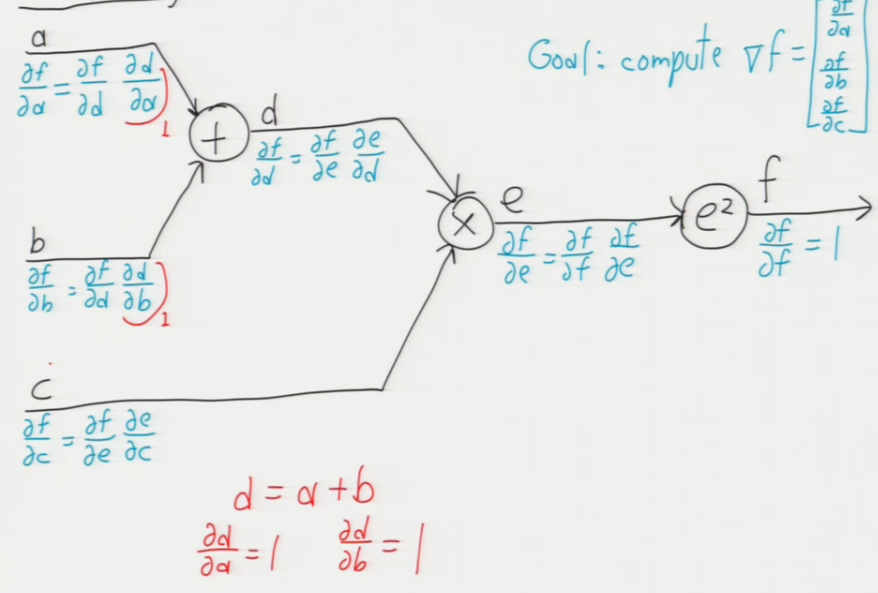
\includegraphics[width=0.6\linewidth]{images/arithmetic_expression_4}
\caption{Arithmetic Expressions}
\label{fig:arithmetic_expression_4}
\end{figure}

I'm gonna do the same thing for $e$ now, $e = cd$, so we have:
\begin{figure}[ht]
\centering
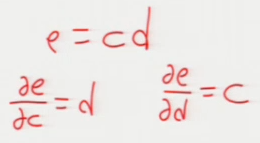
\includegraphics[width=0.2\linewidth]{images/arithmetic_expression_5}
\caption{Arithmetic Expressions}
\label{fig:arithmetic_expression_5}
\end{figure}

Again, we're gonna rewrite those in their proper places:
\begin{figure}[ht]
\centering
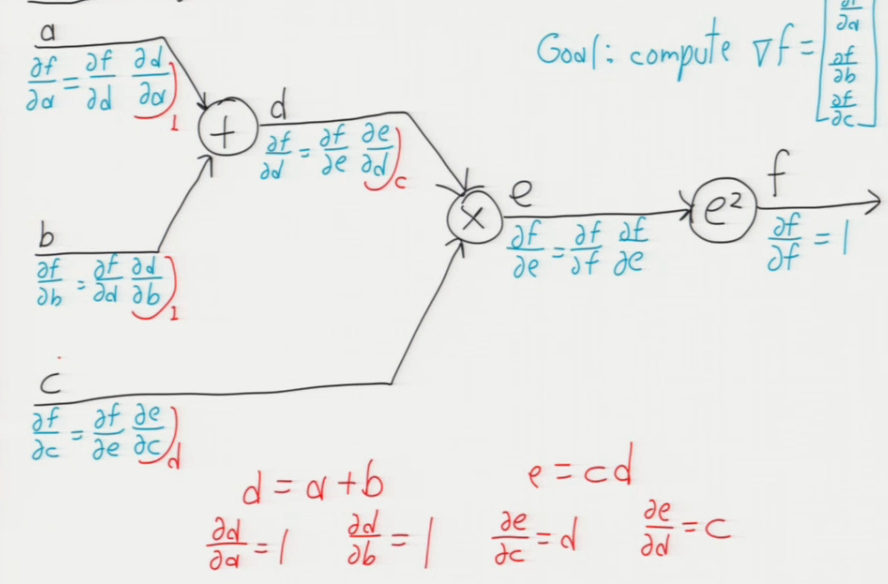
\includegraphics[width=0.6\linewidth]{images/arithmetic_expression_6}
\caption{Arithmetic Expressions}
\label{fig:arithmetic_expression_6}
\end{figure}
\clearpage

And lastly, we have $f = e^2$. And we do the same thing. 
\begin{figure}[ht]
\centering
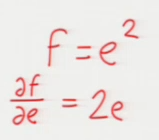
\includegraphics[width=0.2\linewidth]{images/arithmetic_expression_7}
\caption{Arithmetic Expressions}
\label{fig:arithmetic_expression_7}
\end{figure}

So now the diagram looks like:
\begin{figure}[ht]
\centering
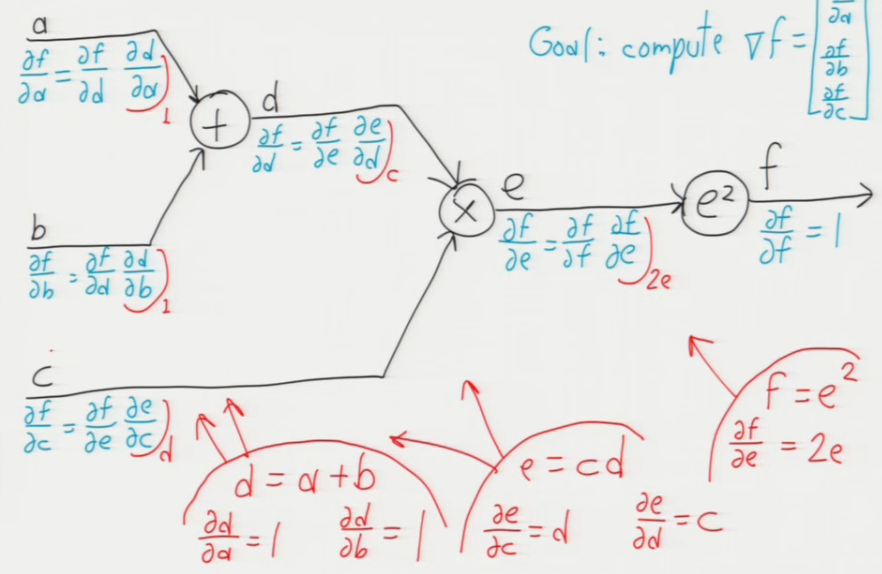
\includegraphics[width=0.6\linewidth]{images/arithmetic_expression_8}
\caption{Arithmetic Expressions}
\label{fig:arithmetic_expression_8}
\end{figure}

As you can see, basically I got one half of all these products done. And so, let's simplify these:
\begin{figure}[ht]
\centering
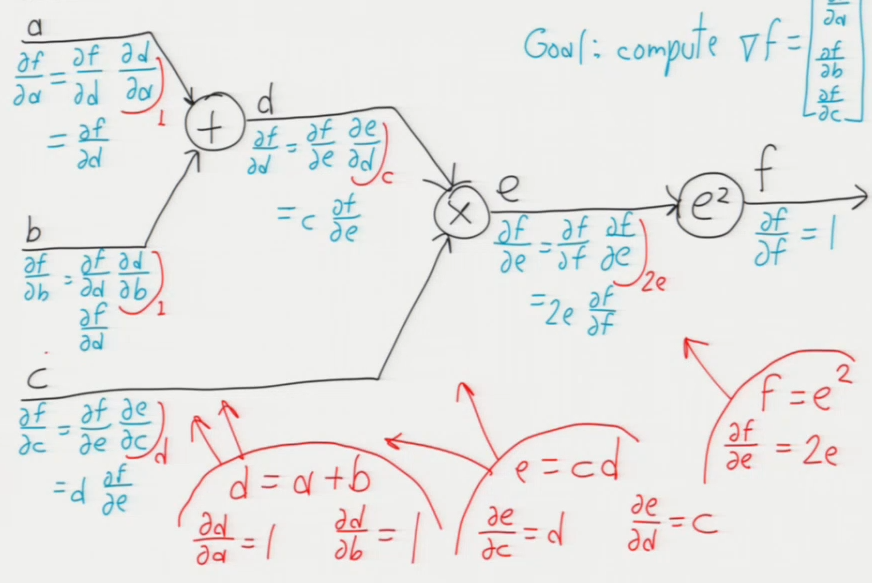
\includegraphics[width=0.6\linewidth]{images/arithmetic_expression_9}
\caption{Arithmetic Expressions}
\label{fig:arithmetic_expression_9}
\end{figure}
\clearpage

So that is as much information as I can figure out about these derivatives on the \textbf{forward-pass}. but we're gonna fill in the rest of these missing values on the \textbf{backward-pass}. And that's the part we call \textbf{backpropagation}.

So, the idea is we start at the end of the circuit, and then we work backward. So, we got $\frac{\partial f}{\partial f} = 1$, we take that and we substitute it in $\frac{\partial f}{\partial e}$, and since we now know what $\frac{\partial f}{\partial e}$ is, we can fill in $\frac{\partial f}{\partial d}$ and $\frac{\partial f}{\partial c}$, and lastly we can fill in $\frac{\partial f}{\partial a}$ and $\frac{\partial f}{\partial b}$. 
\begin{figure}[ht]
\centering
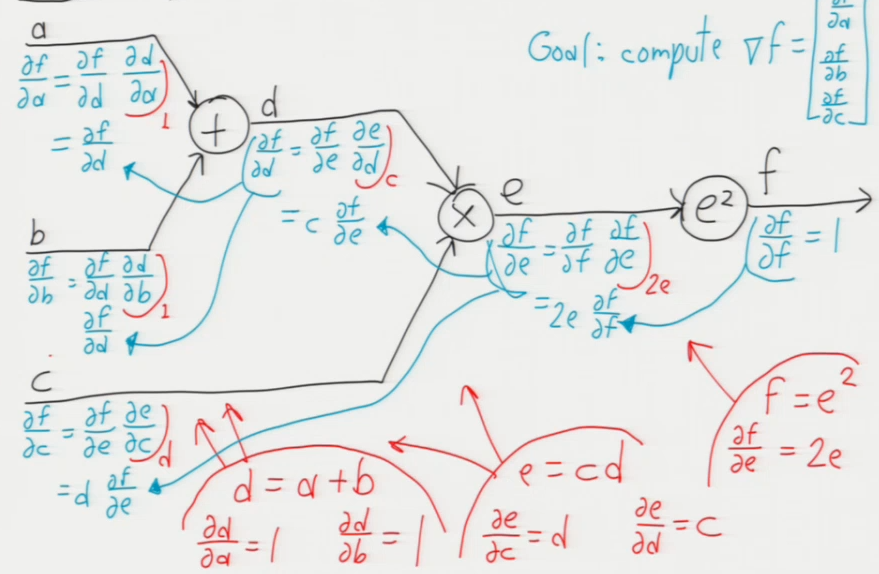
\includegraphics[width=0.6\linewidth]{images/arithmetic_expression_10}
\caption{Arithmetic Expressions}
\label{fig:arithmetic_expression_10}
\end{figure}

And so we now have computed the gradient of $f$. And so one thing I really wanna emphasize is as you can see here these arrows pointing to the left, that is not you write on the paper and do the substitution and figure out what the big long expression is over there and type that expression in your code. No, what happens is at runtime, you're training your neural network, you're gonna compute this number at runtime, then you're gonna go backward and your code will look at the inputs and substitute the appropriate values there, and take that value and substitute it into $a$ and $b$. And this is what allows us to get these derivatives in linear time rather than quadratic time, because of the fact that as we go from right to left, we're computing values in a kinda dynamic-programming-like way where first you're solving this subproblem here, which allows you to solve the subproblem there, which allows you to solve the subproblem there, which looks really much like dynamic programming on a tree. 
\begin{figure}[ht]
\centering
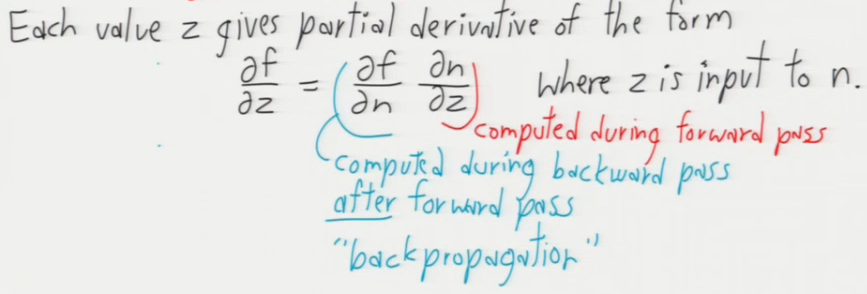
\includegraphics[width=0.6\linewidth]{images/arithmetic_expression_11}
\caption{Arithmetic Expressions}
\label{fig:arithmetic_expression_11}
\end{figure}

So for every value our neural net produces, including intermediate values, we have a partial derivative of this form: the derivative of the loss function or the risk function $f$ over our variable $z$, we ask: well, what is $z$ input to? If it's an input to another variable $n$, then we compute $\frac{\partial f}{\partial n}$ and $\frac{\partial n}{\partial z}$, and we multiply those two things together, it's always the same pattern, and it's always possible to compute $\frac{\partial n}{\partial z}$ during the forward pass. On the other hand, we can backward pass this later on to get $\frac{\partial f}{\partial n}$. And this whole idea is called "backpropagation".
\clearpage

\subsubsection*{More than one unit}
So I want to give you one more example before we go to backpropagation proper because what if a unit's output goes to more than one unit?

I want to do an example that looks more like a neural net. So let's have a unit that actually computes the linear combination just like a neuron does, we're not gonna do the sigmoid yet, we're just gonna do the linear combination part. So I'll have two hidden units that just do linear combinations here. And their inputs are column $x_1$ and $x_2$. And their outputs will go toward a loss function., a square-loss function. 
\begin{figure}[ht]
\centering
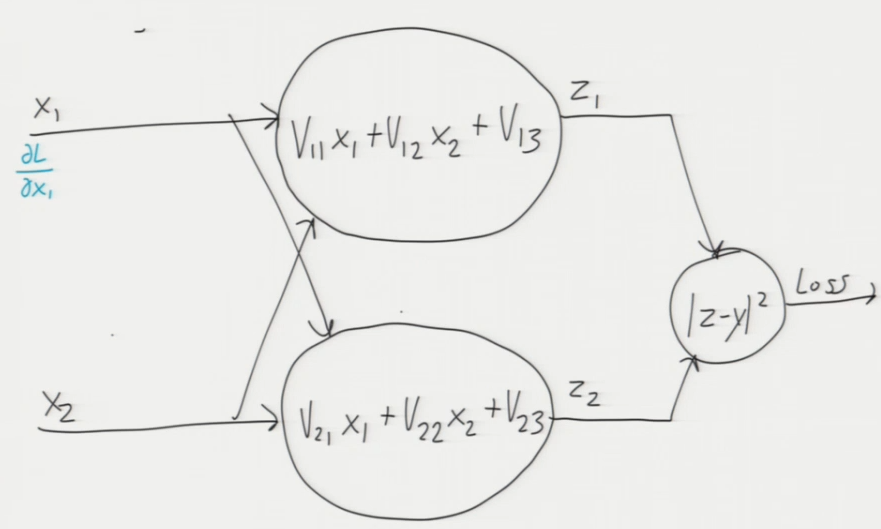
\includegraphics[width=0.7\linewidth]{images/arithmetic_expression_12}
\caption{Arithmetic Expressions}
\label{fig:arithmetic_expression_12}
\end{figure}

So when you do backpropagation for this there's one additional trick that comes up with partial derivatives, which is that our partial derivatives are now more complicated than you'd like them to be because what is the derivative of loss function over $x_1$. in the last example I gave you, the inputs only went into one operator, but now $x_1$ is going into two operators, and so you have to know the rules of calculus and partial derivatives for when $L$ depends on $x_1$ in more than one way. $L$ depends on $x_1$ in two ways through the top neuron and the bottom neuron. So, when you write allthe partial derivative of $L$ w.r.t $x_1$, it's actually going to be a sum of two terms. First, you need the derivative of loss w.r.t to $z_1$ time the derivative of $z_1$ w.r.t $x_1$, but you also need the derivative of the loss w.r.t to the second neuron as well, i.e. $z_2$, and of course, $x_2$ is gonna follow the same rules. 
\begin{figure}[ht]
\centering
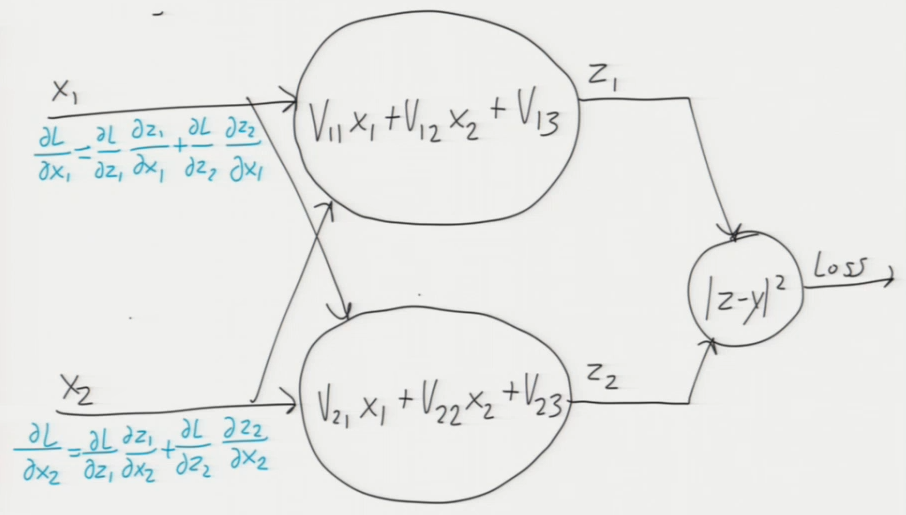
\includegraphics[width=0.7\linewidth]{images/arithmetic_expression_13}
\caption{Arithmetic Expressions}
\label{fig:arithmetic_expression_13}
\end{figure}
\clearpage

Now I can simplify the first one by actually taking the derivatives of $z_1$ w.r.t $x_1$, which is pretty simple, cause that's just a constant.
\begin{figure}[ht]
\centering
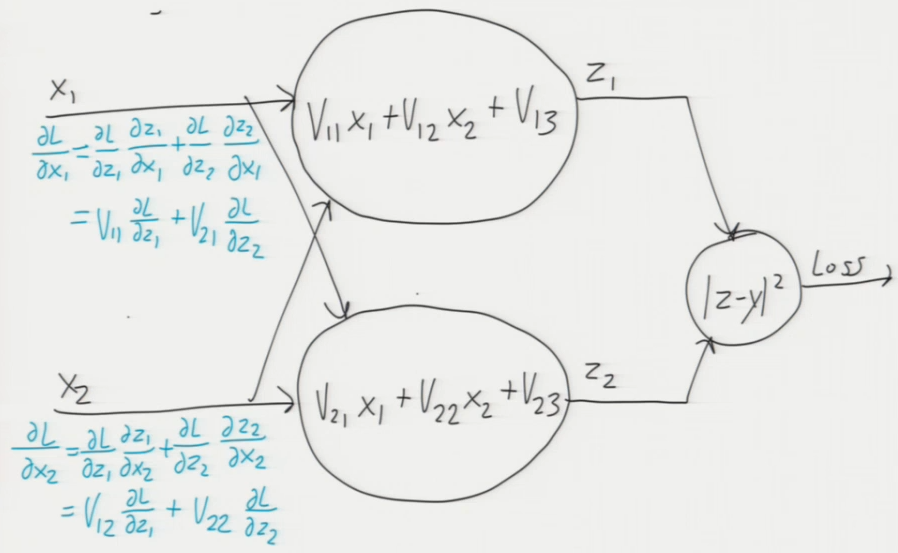
\includegraphics[width=0.7\linewidth]{images/arithmetic_expression_14}
\caption{Arithmetic Expressions}
\label{fig:arithmetic_expression_14}
\end{figure}

So this is as close as I can get to those derivatives during forward propagation. To get the rest of the missing derivatives here, I'm gonna have to go up and do that part of the circuit and then back-prop those derivatives. So at the front end of the circuit, we found out that the derivative of the loss function w.r.t the first hidden unit is $2(z_1 - y_1)$, and the derivative of the loss w.r.t the second hidden unit is $2(z_2 - y_2)$. And having done that I can back-prop those values to where they are needed.
\begin{figure}[ht]
\centering
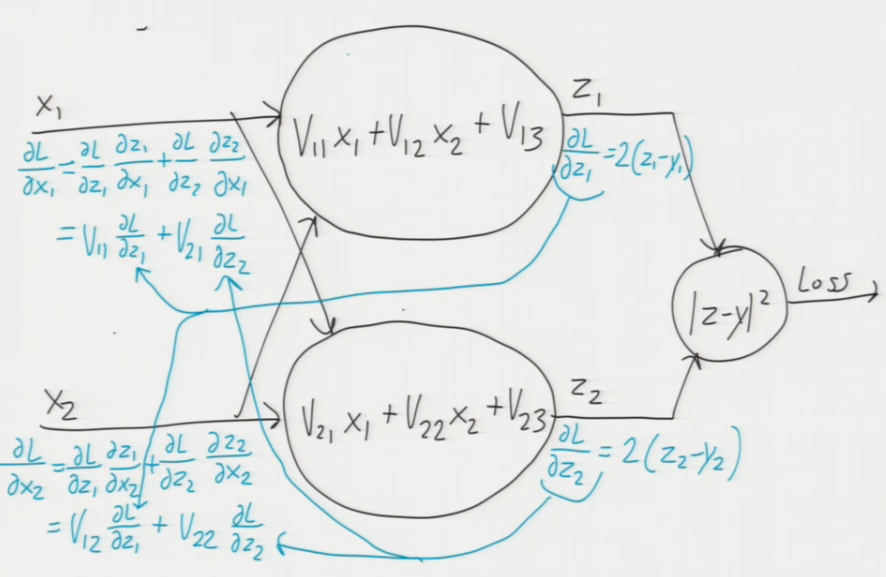
\includegraphics[width=0.7\linewidth]{images/arithmetic_expression_15}
\caption{Arithmetic Expressions}
\label{fig:arithmetic_expression_15}
\end{figure}

So one more time, on the forward pass we compute $x_1$, $x_2$, $z_1$, $z_2$, and the loss. We also have these weights here, which we already know the values of. On the backpropagation step, we take these derivatives here, we backpropagate them to $x_1$ and $x_2$, so we can figure out the gradient of the loss function w.r.t. $x$.
\clearpage

\subsubsection*{Backprogation on Neural Net}
Okay, we're ready to do an actual neural net now. I want to quickly recall a few things. We know the gradient of the logistic function, we're gonna need that. Again, we need to pick a loss function, so we'll use $|z-y|^2$. And I want you to remember from the neural net setup that the hidden unit values are computed by $h_i=s(V_i \cdot x)$, hidden unit $i$ is computed by applying the logistic to row $i$ of the matrix $V$, dot producted with $x$. Therefore, what I can do is I can take the gradient of $h_i$ w.r.t the row of the matrix $V$ that matters here. This will look a little weird here, I'm taking w.r.t one row of a matrix, so we take the row that the hidden unit $i$ depends on, and we're gonna do a gradient w.r.t that row, which tells us how that row should change during gradient descent. By using chain rule, we take the gradient of the logistic function, and then chain rule says you multiply it by the vector $x$ itself. So this gradient is gonna be proportional to the vector $x$.  
\begin{figure}[ht]
\centering
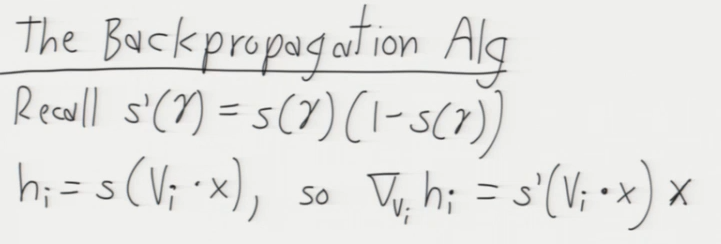
\includegraphics[width=0.7\linewidth]{images/arithmetic_expression_16}
\caption{Arithmetic Expressions}
\label{fig:arithmetic_expression_16}
\end{figure}

So now, let's look at what is the actual back-prop look like as expressions. Once you reduce things to matrix form, it's not all that complicated a circuit. Now you notice this does not look like the neural net I drew you before, the previous neural net form I cared about the numbers, now I care about how the weights change, so now I'm going to draw the weights as the inputs, forget about the $X$'s, for the purpose of training, the $X$'s are constants, so I'm not gonna draw them as inputs cause we don't care about gradients w.r.t X. All we care about is the gradient w.r.t the weights: the weight matrix $V$ and the weight matrix $W$. So from the weights' point of view, this is what the neural net looks like:
\begin{figure}[ht]
\centering
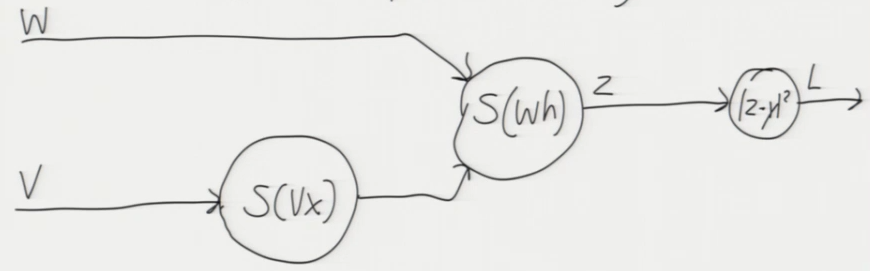
\includegraphics[width=0.7\linewidth]{images/arithmetic_expression_17}
\caption{Arithmetic Expressions}
\label{fig:arithmetic_expression_17}
\end{figure}
\clearpage

This is what the neural net looks like now, that's the whole neural net. It helps that $W$ and $V$ are whole matrices, we can deal with a bunch of variables at once, and now, let's compute the gradients of these things. So, the gradient w.r.t row $i$ of matrix $W$ of the loss function is the derivative of $L$ w.r.t output $z_i$, times the gradient w.r.t $w_i$ of $z_i$. So, we're looking the output of one hidden unit at a time here, and this equation holds for every value of $i$, once for each output unit, and the same thing holds true for $V$. 
\begin{figure}[ht]
\centering
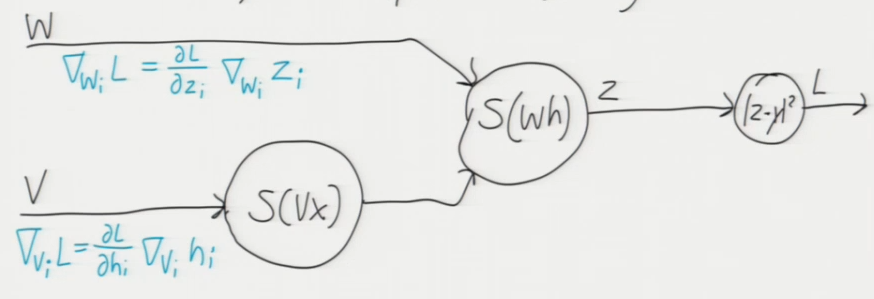
\includegraphics[width=0.7\linewidth]{images/arithmetic_expression_18}
\caption{Arithmetic Expressions}
\label{fig:arithmetic_expression_18}
\end{figure}

So the first one $\triangledown_{w_i} L$, we know the second gradient, we just don't know the first derivative. And likewise, taking the derivative of $L$ w.r.t the weight $V$, I know half of this formula, and I'm missing the other half, which we'll get from backpropagation.
\begin{figure}[ht]
\centering
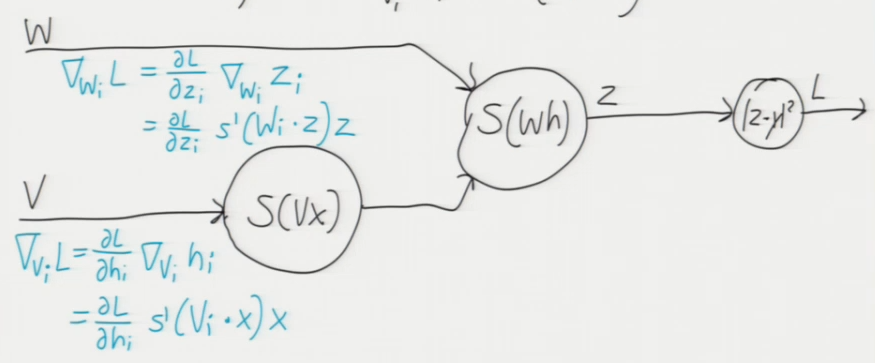
\includegraphics[width=0.7\linewidth]{images/arithmetic_expression_19}
\caption{Arithmetic Expressions}
\label{fig:arithmetic_expression_19}
\end{figure}

I forgot to label it, these are the hidden units $h$. And we need their gradients too: the derivative of the loss function w.r.t the hidden unit $i$ is that summation you recall from the previous section. Now I'll do the summation over all of the output units because every output unit is gonna have an influence on every hidden unit. So this derivative is a sum of all of these products. And again, we can fill in half of those.
\begin{figure}[ht]
\centering
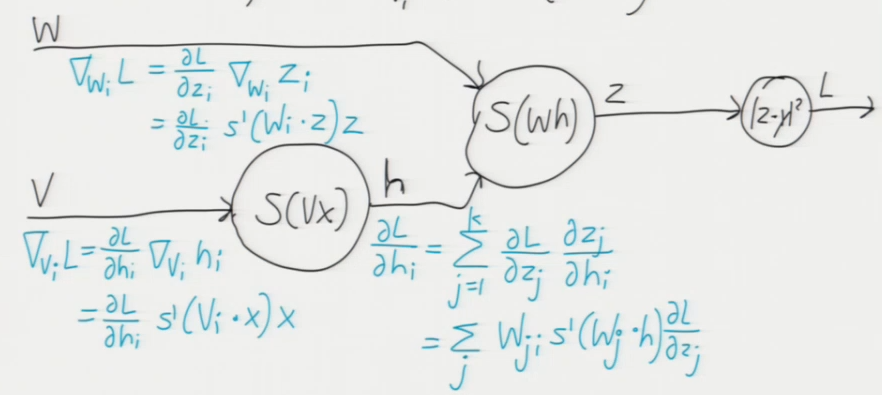
\includegraphics[width=0.7\linewidth]{images/arithmetic_expression_20}
\caption{Arithmetic Expressions}
\label{fig:arithmetic_expression_20}
\end{figure}

\clearpage
And lastly, we need the derivative of the last function in terms of each of the output units. So let's look at one of the output unit $j$, that's the easiest, that just $2(z_j - y_j)$. 
\begin{figure}[ht]
\centering
\includegraphics[width=0.7\linewidth]{images/arithmetic_expression_21}
\caption{Arithmetic Expressions}
\label{fig:arithmetic_expression_21}
\end{figure}

And now, having figured out what these derivatives are, we have half of each derivative when you do backpropagate the other half. Again, we start at the end of the network, where we have the derivative of the loss function w.r.t any particular output neuron, and we propagate that down to here, and we also propagate back to $W$, and, we now also have the derivate of the loss function w.r.t each of our hidden units. And so we take that and we backpropagate that to $V$ to get the derivatives of the weights in the matrix $V$. 
\begin{figure}[ht]
\centering
\includegraphics[width=0.7\linewidth]{images/arithmetic_expression_22}
\caption{Arithmetic Expressions}
\label{fig:arithmetic_expression_22}
\end{figure}

And even though I've done this with just one layer of hidden units, the exact same pattern just repeats itself, if you say like 5 layers of hidden units. That doesn't change at all. So you can take this idea here, and just extend it by adding additional stages of hidden units, and it's all the same.  
\clearpage

\section*{Neural Network: A Simpler Explanation}
Let's say we're now looking at a neural network like this:

\subsection*{Backpropagation}
\begin{description}
\item [Idea: ] update each of the weights in the network so that they cause the actual output to be closer to the target output, thereby minimizing the error for each output neuron and the network as a whole
\end{description}

\subsubsection*{Output Layer}
Consider $w_5$, we wanna know how much a change in $w_5$ affects the total error, aka $\frac{\partial E_{total}}{\partial w_5}$. And by chain rule, we have
$$\frac{\partial E_{total}}{\partial w_5} = 
\color{red}{\frac{\partial E_{total}}{\partial out_{o_1}}} \cdot
\color{green}{\frac{\partial out_{o_1}}{\partial net_{o_1}}} \cdot
\color{blue}{\frac{\partial net_{o_1}}{\partial w_5}}
$$

Let's start with $\frac{\partial E_{total}}{\partial out_{o_1}}$, i.e. we wanna find how much does the total error change w.r.t to the output.
$$E_{total} = \frac{1}{2}(target_{o_1} - out_{o_1})^2 + \frac{1}{2}(target_{o_2} - out_{o_2})^2$$
So we have
$$
\begin{aligned}
\mathbf{\color{red}{\frac{\partial E_{total}}{\partial out_{o_1}}}} 
& = 2 \cdot \frac{1}{2}(target_{o_1} - out_{o_1}) \cdot (-1) + 0 \\
& = -target_{o_1} + out_{o_1} \\
& = -(0.01 - 0.75136507) \\
& = 0.74136507
\end{aligned}
$$

As for $\frac{\partial out_{o_1}}{\partial net_{o_1}}$, we have
$$
out_{o_1} = \frac{1}{1 + e^{-net_{o_1}}}
$$

And recall for sigmoid function $r(x) = \frac{1}{1+e^{-x}}$,
$$r'(x) = r(x)(1 - r(x)))$$

So,
$$
\begin{aligned}
\mathbf{\color{green}{\frac{\partial out_{o_1}}{\partial net_{o_1}}}}
& = out_{o_1}(1-out_{o_1}) \\
& = 0.75136505 \cdot (1-0.75136507) \\
& = 0.186815602
\end{aligned}
$$

Lastly, for $\frac{\partial net_{o_1}}{\partial w_5}$, we have
$$
net_{o_1} = w_5 \cdot out_{h_1} + w_6 \cdot out_{h_2}
$$

So,
$$
\begin{aligned}
\mathbf{\color{blue}{\frac{\partial net_{o_1}}{\partial w_5}}}
& = out_{h_1} \\
& = 0.593269992
\end{aligned}
$$

Putting them altogether, we have 0.082167041.

To decrease the error, subtract this value from the current weight:
$$
\begin{aligned}
\mathbf{w_5^+}
& = w_5 - \alpha \cdot \frac{\partial E_{total}}{\partial w_5} \\
& = 0.4 - 0.5 * 0.082167041
& = 0.35891648
\end{aligned}
$$

Repeat for $w_6^+$, $w_7^+$ and $w_8^+$, we have:
$$w_6^+ = 0.408666186$$
$$w_7^+ = 0.511301270$$
$$w_8^+ = 0.561370121$$

\subsubsection*{Hidden Layer}
Big picture, here's what we need to figure out:
$$
net_{o_1} = w_5 * h1 + w_6 * h2 + b_2 * 1
$$
$$
out_{o_1} = \frac{1}{1 + e^{-net_{o_1}}}
$$
$$E_{total} = \frac{1}{2}(target_{o_1} - out_{o_1})^2 + \frac{1}{2}(target_{o_2} - out_{o_2})^2$$

\section*{Convolutional Neural Network}
Convolutional Neural Networks are very similar to ordinary Neural Networks: 
\begin{itemize}
\item they are made up of neurons that have learnable weights and biases.
\item Each neuron receives some inputs, performs a dot product and optionally follows it with a non-linearity.
\item The whole network still expresses a single differentiable score function: from the raw image pixels on one end to class scores at the other.
\item And they still have a loss function (e.g. SVM/Softmax) on teh last layer and all the tips/tricks we developed for learning regular Neural Networks still apply.
\end{itemize}

So what does change? ConvNet architectures make the explicit assumption that the inputs are images, which allows us to encode certain properties into the architecture. These then make the forward function more efficient to implement and vastly reduce the amount of parameters in the network.

\subsection*{Architecture Overview}
Recall: \textbf{\textit{Regular Neural Nets}}. As we saw in the previous chapter, Neural Networks receive an input (a single vector), and transform it through a series of \textbf{\textit{hidden layers}}. Each hidden layer is made up of a set of neurons, where each neuron is fully connected to all neurons in the previous layer, and where neurons in a single layer function completely independently and do not share any connections. The last fully-connected layer is called the "output layer" and in classification settings it represents the class scores.\medskip

\textbf{\textit{Regular Neural Nets don't scale well to full images.}} In CIFAR-10, images are only size 32x32x3 (32 wide, 32 high, 3 color channels), so a single fully-connected neuron in a first hidden layer of a regular Neural Network would have 32*32*3 = 3072 weights. This amount still seems manageable, but clearly this fully-connected structure does not scale to larger images. For example, an image of more respectable size, e.g. 200x200x3, would lead to neurons that have 200*200*3=120000 weights. Moreover, we would almost certainly want to have several such neurons, so the parameters would add up quickly! Clearly, this full connectivity is wasteful and the huge number of parameters would quickly lead to overfitting.\medskip

\textbf{\textit{3D volumes of neurons.}} Convolutional Neural Networks take advantage of the fact that the inputs consists of images and they constrain the architecture in a more sensible way. In particular, unlike a regular Neural Network, the layers of a ConvNet have neurons arranged in 3 dimensions: \textbf{width, height, depth}. (Note that the word \textbf{\textit{depth}} here refers to the third dimension of an activation volume, not to the depth of a full Neural Network, which can refer to the total number of layers in a network.) For example, the input images in CIFAR-10 are an input volume of activations, and the volume has dimensions 32x32x3 (width, height, depth respectively).
As we will soon see, the neurons in a layer will only be connected to a small region of the layer before it, instead of all of the neurons in a fully- connected manner. Moreover, the final input layer would for CIFAR-10 have dimensions 1x1x10, because by the end of the ConvNet architecture we will reduce the full image into a single vector of class scores, arranged along the depth dimension.Here is a visualization:

\begin{figure}[ht]
\centering
\includegraphics[width=0.7\linewidth]{images/cnn}
\caption{A regular 3-layer Neural Network.}
\label{fig:Sample Neural Neural Network}
\end{figure}

\begin{figure}[ht]
\centering
\includegraphics[width=0.7\linewidth]{images/neural_net2}
\caption{A ConvNet arranges its neurons in three dimensions (width, height, depth), as visualized in one of the layers. Every layer of a ConvNet transforms the 3D input volume to a 3D output volume of neuron activations. In this example, the red input layer holds the image, so its width and height would be the dimensions of the image, and the depth would be 3 (Red, Green, Blue Channels).}
\label{fig:Sample ConvNet}
\end{figure}

\begin{quote}
A ConvNet is made up of Layers. Every Layer has a simple API: It transforms an input 3D volume to an output 3D volume with some differentiable function that may or may not have parameters.
\end{quote}

\subsection*{Layer used to build ConvNets}
As we described above, a simple ConvNet is a sequence of layers, and every layer of a ConvNet transforms one volume of activations to another through a differentiable function. We use three main types of layers to build ConvNet architectures: 
\begin{enumerate}
\item Convolutional Layer
\item Pooling Layer
\item Fully-Connected Layer (exactly as seen in regular Neural Networks)
\end{enumerate}
We will stack these layers to form a full ConvNet architecture.

\textbf{\textit{Example Architecture Overview:}} We will go into details below, but a simple ConvNet for CIFAR-10 classification could have the architecture \textbf{[INPUT-CONV-RELU-POOL-FC]}. In more detail:\medskip

\begin{itemize}
\item \textbf{INPUT [32x32x3]} will hold the raw pixel values of the image, in this case an image of width 32, height 32, and with three color channels R, G, B.
\item \textbf{CONV layer} will compute the output of neurons that are connected to local regions in the input, each computing a dot product between their weights and a small region they are connected to in the input volume. This may result in volume such as \textbf{[32x32x12]} if we decided to use 12 filters.
\item \textbf{RELU layer} will apply an elementwise activation function, such as the \(\mathbf{max(0,x)}\) thresholding at zero. This leaves the size of the volume unchanged (\textbf{[32x32x12]}).
\item \textbf{POOL layer} will perform a downsampling operation along the spatial dimensions (width, height), resulting in volume such as \textbf{[16x16x12]}.
\item \textbf{FC (i.e. fully-connected) layer} will compute the class scores, resulting in volume of size \textbf{[1x1x10]}, where each of the 10 numbers correspond to a class score, such as among the 10 categories of CIFAR-10. As with ordinary Neural Networks and as the name implies, each neuron in this layer will be connected to all the numbers in the previous volume.
\end{itemize}

In this way, ConvNets transform the original image layer by layer from the original pixel values to the final class scores. Note that some layers contain parameters and other don't. In particular, the CONV/FC layers perform transformations that are a function of not only the activations in the input volume, but also of the parameters (the weights and biases of the neurons). On the other hand, the RELU/POOL layers will implement a fixed function. The parameters in the CONV/FC layers will be trained with gradient descent so that the class scores that the ConvNet computes are consistent with the labels in the training set for each image.\medskip

In summary:
\begin{itemize}
\item A ConvNet architecture is in the simplest case a list of Layers that transform the image volume into an output volume (e.g. holding the class scores)
\item There are a few distinct types of Layers (e.g. CONV/FC/RELU/POOL are by far the most popular)
\item Each Layer accepts an input 3D volume and transform it to an output 3D volume through a differentiable function
\item Each Layer may or may not have parameters (e.g. CONV/FC do, RELU/POOL don't)
\item Each Layer may or may not have additional hyperparameters (e.g. CONV/FC/POOL do, RELU doesn't)
\end{itemize}

\begin{figure}[ht]
\centering
\includegraphics[width=1.0\linewidth]{images/convnet}
\caption{The activations of an example ConvNet architecture. The initial volume stores the raw image pixels (left) and the last volume stores the class scores (right). Each volume of activations along the processing path is shown as a column. Since it's dificult to visualize 3D volumes, we lay out each volume's slices in rows. The last layer volume holds the scores for each class, but here we only visualize the sorted top 5 scores, and print the labels of each one. The full web-based demo is shown in the header of our website. The architecture shown here is a tiny VG net, which we will discuss later.}
\label{fig:Example ConvNet architecture}
\end{figure}

We now describe the individual layers and the details of their hyperparameters and their connectivities.

\subsection*{Covolutional Layer}
The Conv layer is the core building block of a Convolutional Network that does most of the computational heavy lifting.\medskip

\textbf{Overview and intuition without brain stuff.} Let's first discuss what the CONV layer computes without brain/neuron analogies. The CONV layer's parameters consist of a set of learnable filters. Every filter is small spatially (along width and height), but extends through the full depth of the input volume. For example, a typical filter on a first layer of a ConvNet might have size 5x5x3 (i.e. 5 pixels width and height, and 3 because images have depth 3, the color channels). During the forward pass, we slide (more precisely, convolve) each filter across the width and height of the input volume and compute dot products between the entries of the filter and the input at any position. As we slide the filter over the width and height of the input volume we will produce a 2-dimensional activation map that gives the responses of that filter at every spatial position. Intuitively, the network will learn filters that activate when they see some type of visual feature such as an edge of some orientation or a blotch of some color on the first layer, or eventually entire honey comb or wheel-like patterns on higher layers of the network. Now, we will have an entire set of filters in each CONV layer (e.g. 12 filters), and each of them will produce a separate 2-dimensional activation map. We will stack these activation maps along the depth dimension and produce the output volume.\medskip

\textbf{The brain view.} If you're a fan of the brain/neuron analogies, every entry in the 3D output volume can also be interpreted as an output of a neuron that looks at only a small region in the input and shares parameters with all neurons to the left and right spatially (since these numbers all result from applying the same filter). We now discuss the details of the neuron connectivities, their arrangement in space, and their parameter sharing scheme.

\textbf{Local Connectivity.} When dealing with high-dimensional inputs such as images, as we saw above it is impractical to connect neurons to all neurons in the previous volume. Instead, we will connect each neuron to only a local region of the input volume. The spatial extent of this connectivity is a hyperparameter called the \textbf{receptive field} of the neuron (equivalently this is the filter size). The extent of the connectivity along the depth axis is always equal to the depth of the input volume. It is important to emphasize again this asymmetry in how we treat the spatial dimensions (width and height) and the depth dimension: The connections are local in space (along width and height), but always full along the entire depth of the input volume.

\textbf{\textit{Example 1.}} For example, suppose that the input volume has size \textbf{[32x32x3]}, (e,g, an RGB CIFAR-10 image). If the receptive field (or the filter size) is 5x5, then each neuron in the Conv Layer will have weights to a [5x5x3] region in the input volume, for a total of 5*5*3=75 weights (and +1 bias parameter). Notice that the extent of the connectivity along the depth axis must be 3, since this is the depth of the input volume.

\textbf{\textit{Example 2.}} Suppose an input volume has size \textbf{[16x16x20]}. Then using an example receptive field size of 3x3, every neuron in the Conv Layer would now have a total of 3*3*20=180 connections to the input volume. Notice that, again, the connectivity is local in space (e.g. 3x3), but full along the input depth (20).

\begin{figure}[ht]
\centering
\includegraphics[width=0.7\linewidth]{images/depthcol}
\caption{An example input volume in red (e.g. a 32x32x3 CIFAR-10 image), and an example volume of neurons in the first Convolutional layer. Each neuron in the convolutional layer is connected only to a local region in the input volume spatially, but to the full depth (i.e. all color channels). Note, there are multiple neurons (5 in this example) along the depth, all looking at the same region in the input - see discussion of depth columns in text below.}
\label{fig:Example Input Volume}
\end{figure}

\begin{figure}[ht]
\centering
\includegraphics[width=0.7\linewidth]{images/neuron_model}
\caption{The neurons from the Neural Network chapter remain unchanged: They still compute a dot product of their weights with the input followed by a non-linearity, but their connectivity is now restricted to be local spatially.}
\label{fig:Example Neurons}
\end{figure}

\textbf{Spatial arrangement.} We have explained the connectivity of each neuron in the Conv Layer to the input volume, but we haven't yet discussed how many neurons there are in the output volume or how they are arranged. Three hyperparameters control the size of the output volume: the \textbf{depth}, \textbf{stride} and \textbf{zero-padding}. We discuss these next:

\begin{enumerate}
\item First, the \textbf{depth} of the output volume is a hyperparameter: it corresponds to the number of filters we would like to use, each learning to look for something different in the input. 
\end{enumerate}

\section*{Convolutional Neural Network (Udemy)}
\subsection*{Translational Invariance}

\subsection*{Pooling}
Another import operation we'll need before we build the convolutional neural network is \textbf{downsampling}.

First, importing all the packages needed.

\begin{lstlisting}[language=Python, caption=Importing]
# Import the stuff
import os
import numpy as np
import theano
import theano.tensor as T
import matplotlib.pyplot as plt

from theano.tensor.nnet import conv2d
from theano.tensor.signal import pool

from scipy.io import loadmat
from sklearn.utils import shuffle

from datetime import datetime
\end{lstlisting}

The first method we're looking at reads the data. 

\begin{lstlisting}[language=Python, caption=Getting Data]
def get_data():
    """Reads dataset
    
    Retrieves the dataset
    
    Returns:
        A tuple containing the training set (dict) and the testing set (dict)
    """
    if not os.path.exists('../large_files/House_Numbers/train_32x32.mat')
        print('Looking for ../large_files/House_Numbers/train_32x32.mat')
        print('You have not downloaded the data and/or not placed the files in the correct location.')
        print('Please get the data from: http://ufldl.stanford.edu/housenumbers')
        print('Place train_32x32.mat and test_32x32.mat in the folder large_files adjacent to the class folder')
        exit()

    train = loadmat('../large_files/House_Numbers/train_32x32.mat')
    test  = loadmat('../large_files/House_Numbers/test_32x32.mat')
    return train, test  
\end{lstlisting}

This method rearranges the dimensions of data for Theano.

\begin{lstlisting}[language=Python, caption=Rearranging Dimensions]
def rearrange(X):
    """Rearranges the matrix
    
    Rearranges the matrix into a different dimension. For example:
    
    Input is (32, 32, 3, N)
    Output is (N, 3, 32, 32)
    
    In this case, N is the number of color images (3 color channels) with
    a size of 32 x 32. Instead of using a matrix of size 32 x 32 x 3 x N,
    we rearrange it as N x 3 x 32 x 32
    
    Args:
        X: a numpy.ndarray matrix with 4 dimensions
        
    Returns:
        A rearranged numnpy.ndarray matrix
    """
    return (X.transpose(3, 2, 0, 1) / 255).astype(np.float32)
\end{lstlisting}

The next method we're looking at initiates a kernel filter.

\begin{lstlisting}[language=Python, caption=Initing an Filter]
def init_filter(shape, poolsz):
    """Initializes a filter
    
    Takes in the shape and pooling size and generates a filter
    with the same dimensions as `shape`
    
    Args:
        shape: a tuple specifying the dimension
        poolsz: a tuple specigying the pooling size
    Returns:
        A numpy.ndarray containing the filter
    """
    w = np.random.randn(*shape) * np.sqrt(2.0 / np.prod(shape[]1:))
    return w.astype(np.float32)
\end{lstlisting}

Then we define our RELU function.

\begin{lstlisting}[language=Python, caption=RELU]
def relu(a):
    return a * (a > 0)
\end{lstlisting}

Next, we pipe Convolution and Pooling altogether.

\begin{lstlisting}[language=Python, caption=Convolution and Pooling]
def convpool(X, W, b, poolsize=(2,2)):
    conv_out = conv2d(input=X, filters=W)
    
    # downsample each feature map individually, using maxpooling
    pooled_out = pool.pool_2d(
        input=conv_out,
        ws=poolsize,
        ignore_border=True
    )
    
    # add the bias term. Since the bias is a vector (1D array), we first
    # 
\end{lstlisting}

\begin{lstlisting}[language=Python, caption=Theano example]


def main():
    # Overview of the network
    """
    Input: 32 x 32 x 3 x N
    
    """
    
    # Step 1 
    # Load the data, transform as needed
    train, test = get_data()
    
    # Need to scale! Don't leave as 0..255
    # Y is a N x 1 matrix with values 1..10 (Matlab indexes by 1)
    # So flatten it and make it 0..9
    # Also need indicator matrix for cost calculation
    Xtrain = rearrange(train['X']) # (N, 3, 32, 32)
    Ytrain = test['y'].flatten() - 1
    del train
    Xtrain, Ytrain = shuffle(Xtrain, Ytrain)
    
    Xtest = rearrange(test['X'])
    Ytest = test['y'].flatten() - 1
    del test
    
    max_iter = 20
    print_period = 10
    
    # learning rate
    lr = np.float32(1e-2)
    # regularization = 0.01
    # momentum
    mu = np.float32(0.99)
    
    N = Xtrain.shape[0]
    batch_sz = 500
    n_batches = N // batch_sz
    
    # at our last stage, the fully connected NN layer has 500 hidden units
    M = 500
    # and 10 outputs
    K = 10
    poolsz = (2, 2)
    
    
\end{lstlisting}

\pagebreak

\section*{Signals and Systems}

\href{https://ocw.mit.edu/resources/res-6-007-signals-and-systems-spring-2011/}{MIT Link}
\href{https://www.youtube.com/playlist?list=PL41692B571DD0AF9B}{YouTube Playlist}

\subsection*{Lecture 1: Introduction}

\pagebreak

\subsection*{Lecture 2: Signals and systems: Part I}

Mathematically, the continuous sinusoidal signal is expressed as:

$$x(t) = A cos (\omega_0 t + \phi)$$

where $A$ is the amplitude, $\omega$ is the frequency and $\phi$ is the phase.

Graphically, the sinusoidal signal has the form as show here:

\begin{figure}[ht]
\centering
\includegraphics[width=0.5\linewidth]{images/signals_01.png}
\caption{Continuous Sinusoidal Signal}
\label{fig:signals_01}
\end{figure}

One of the properties of sinusoidal signal is it's periodic, i.e., under an appropriate time shift, $T_0$, the signal replicates or repeats itself:

$$x(t) = x(t + T_0) \quad \text{period} \triangleq \text{small}$$

To demonstrate that, we substitute $T_0$ into the expression:

\begin{proof}
$$
\begin{aligned}
x(t + T_0)
& = A cos [\omega_0 (t + T_0) + \phi] \\
& = A cos [\omega_0 t + \omega_0 T_0 + \phi]
\end{aligned}
$$
\end{proof}

One of the things we know about sinusoidal functions is that if we change the argument by any integer multiple of $2 \pi$, then the function has the same value. So we can exploit that and  if:

$$\omega_0 T_0 = 2 \pi m$$

then the right hand side of the equation will be the same as the original signal. So with

$$T_0 = \frac{2 \pi m}{\omega_0}$$ 

the signal becomes the same and we can say the period is $\frac{2 \pi}{\omega_0}$.

In addition, another useful property of the sinusoidal signal is that a time shift of a sinusoid is equivalent to a phase change. If we put the sinusoidal signal under a time shift of small $t_0$, and expands it out, we get:

$$A cos[\omega_0 (t+t_0)] = A cos[\omega_0 t + \omega_0 t_0]$$

and we can see it's equivalent to a change in phase. And not only is a time shift generating a phase change, but in fact, if we insert a phase change, there's always a $t_0$ which would correspond to an equivalent time shift, i.e., if we take $\omega_0t_0$ and think of that as a change in phase, for any change in phase, we can solve this equation for time shift:

$$\omega_0 t_0 = \phi$$

\begin{figure}[ht]
\centering
\includegraphics[width=0.5\linewidth]{images/signals_02.png}
\caption{Continuous Sinusoidal Signal Relationships}
\label{fig:signals_02}
\end{figure}

And an important thing to recognize about this statement is that not only is a time shift generating a phase change, but, in fact, if we inserted a phase change, there is always a value of $t_0$ which would correspond to an equivalent time shift. Said another way, if we take $\omega_0 t_0$ and think of that as our change in phase, for any change in phase, we can solve this equation for a time shift, or conversely for any value of time shift, that represents an appropriate phase.

So a time shift corresponds to a phase change, and a phase change, likewise, corresponds to time shift. And so for example, if we look at the general sinusoidal signal that we saw previously, in effect, changing the phase corresponds to moving this signal in time one way or the other. For example, if we look at the sinusoidal signal with a phase equal to 0 that corresponds to locating the time origin at this peak. And I've indicated that on the following graph. (Look at Figure ~\ref{fig:signals_03})

\begin{figure}[ht]
\centering
\includegraphics[width=0.45\linewidth]{images/signals_03.png}
\caption{Illustration of the signal $A cos w_o t$ as an even signal.}
\label{fig:signals_03}
\end{figure}

So here we have illustrated a sinusoid with 0 phase, or a cosine with 0 phase, corresponding to taking our general picture and shifting it. Shifting it appropriately as I've indicated here. This, of course, still has the property that it's a periodic function, since we simply displaced it in time.

And by looking at the graph, what we see is that it has another very important property, a property referred to as even. And that's a property that we'll find useful, in general, to refer to in relation to signals. A signal is said to be even if, when we reflect it about the origin, it looks exactly the same. So it's symmetric about the origin.

And looking at this sinusoid, that, in fact, has that property. And mathematically, the statement that it's even is equivalent to the statement that if we replace the time argument by its negative, the function itself doesn't change.

Now this corresponded to a phase shift of 0 in our original cosine expression. If instead, we had chosen a phase shift of, let's say, $-\pi/2$, then instead of a cosinusoidal signal, what we would regenerate is a sinusoid with the appropriate phase. Or, said another way, if we take our original cosine and substitute in for the phase $-\pi/2,$ then of course we have this mathematical expression. (Look at Figure ~\ref{fig:signals_04})

\begin{figure}[ht]
\centering
\includegraphics[width=0.5\linewidth]{images/signals_04.png}
\caption{Illustration of the signal $A sin w_o t$ as an odd signal.}
\label{fig:signals_04}
\end{figure}

Using just straightforward trigonometric identities, we can express that alternately as $sin(\omega_0*t)$. The frequency and amplitude, of course, haven't changed. And that, you can convince yourself, also is equivalent to shifting the cosine by an amount in time that I've indicated here, namely a quarter of a period.

So illustrated below (Still in Figure ~\ref{fig:signals_04}) is the graph now, when we have a phase of $-\pi/2$ in our cosine, which is a sinusoidal signal. Of course, it's still periodic. It's periodic with a period of $2 \pi / \omega_0$ again, because all that we've done by introducing a phase change is introduced the time shift.

Now, when we look at the sinusoid in comparison with the cosine, namely with this particular choice of phase, this has a different symmetry, and that symmetry is referred to odd. What odd symmetry means, graphically, is that when we flip the signal about the time origin, we also multiply it by a minus sign. So that's, in effect, anti-symmetric. It's not the mirror image, but it's the mirror image flipped over. And we'll find many occasions, not only to refer to signals more general than sinusoidal signals, as even in some cases and odd in other cases. And in general, mathematically, an odd signal is one which satisfies the algebraic expression, $x(t)$. When you replace t by its negative, is equal to $-x(-t)$. So replacing the argument by its negative corresponds to an algebraic sign reversal.

OK. So this is the class of continuous-time sinusoids. We'll have a little more to say about it later. But I'd now like to turn to discrete-time sinusoids. What we'll see is that discrete-time sinusoids are very much like continuous-time ones, but also with some very important differences. And we want to focus, not only on the similarities, but also on the differences.

Well, let's begin with the mathematical expression. A discrete-time sinusoidal signal, mathematically, is as I've indicated here, $A cos(\omega_0 n + \phi)$. And just as in the continuous-time case, the parameter $A$ is what we'll refer to as the amplitude, $omega_0$ as the frequency, and $\phi$ as the phase. (Look at Figure ~\ref{fig:signals_05})

\begin{figure}[ht]
\centering
\includegraphics[width=0.5\linewidth]{images/signals_05.png}
\caption{Illustration of discrete-time sinusoidal signals.}
\label{fig:signals_05}
\end{figure}

And I've illustrated here several discrete-time sinusoidal signals. And they kind of look similar. In fact, if you track what you might think of as the envelope, it looks very much like what a continuous-time sinusoid might look like. But keep in mind that the independent variable, in this case, $n$, is an integer variable. And so the sequence only takes on values at integer values of the argument. And we'll see that has a very important implication, and we'll see that shortly.

Now, one of the issues that we addressed in the continuous-time case was periodicity. And I want to return to that shortly, because that is one of the areas where there is an important distinction. Let's first, though, examine the statement similar to the one that we examined for continuous time, namely the relationship between a time shift and a phase change.

Now, in continuous time, of course, we saw that a time shift corresponds to a phase change, and vice versa. Let's first look at the relationship between shifting time and generating a change in phase. In particular for discrete time, if I implement a time shift that generates a phase change, and we can see that easily by simply inserting a time shift, $n + n_0$. And if we expand out this argument, we have $\omega_0 n + \omega_0 n_0$. (Look at Figure ~\ref{fig:signals_06})

\begin{figure}[ht]
	\centering
	\includegraphics[width=0.4\linewidth]{images/signals_06.png}
	\caption{Relationship between a time shift and a phase change for discrete-time sinusoidal signals. In discrete time, a time shift always implies a phase change.}
	\label{fig:signals_06}
\end{figure}

And so I've done that on the right-hand side of the equation here. And the $\omega_0 n_0$, then, simply corresponds to a change in phase. So clearly, a shift in time generates a change in phase.

And for example, if we take a particular sinusoidal signal, let's say we take the cosine signal at a particular frequency, and with a phase equal to 0, a sequence that we might generate is one that I've illustrated here. So what I'm illustrating here is the cosine signal with 0 phase. And it has a particular behavior to it, which will depend somewhat on the frequency. (Look at Figure ~\ref{fig:signals_07})

\begin{figure}[ht]
	\centering
	\includegraphics[width=0.5\linewidth]{images/signals_07.png}
	\caption{Relationship between a time shift and a phase change for discrete-time sinusoidal signals. In discrete time, a time shift always implies a phase change.}
	\label{fig:signals_07}
\end{figure}

If I now take this same sequence and shift it so that the time origin is shifted a quarter of a period away, then you can convince yourself-- and it's straightforward to work out-- that that time shift corresponds to a phase shift of $\pi / 2$. So in that case, with the cosine with a phase of $-\pi / 2$, that will correspond to the expression that I have here.

\begin{figure}[ht]
	\centering
	\includegraphics[width=0.6\linewidth]{images/signals_08.png}
	\caption{The sequence $A sin \omega_0 n$ illustrating the antisymmetric property of an odd sequence.}
	\label{fig:signals_08}
\end{figure}

We could alternately write that, using again a trigonometric identity, as a sine function. And that, I've stated, is equivalent to a time shift. Namely, this shift of $ \pi/2$ is equal to a certain time shift, and the time shift for this particular example is a quarter of a period.

So here, we have the sinusoid. Previously we had the cosine. The cosine was exactly the same sequence, but with the origin located here. And in fact, that's exactly the way we drew this graph. Namely, we just simply took the same values and changed the time origin.

Now, looking at this sequence, which is the sinusoidal sequence, the phase of $-\pi/2$, that has a certain symmetry. And in fact, what we see is that it has an odd symmetry, just as in the continuous-time case. Namely, if we take that sequence, flip it about the axis, and flip it over in sign, that we get the same sequence back again. Whereas with 0 phase corresponding to the cosine that I showed previously, that has an even symmetry. Namely, if I flip it about the time origin and don't do a sign reversal, then the sequence is maintained.

So here, we have an odd symmetry, expressed mathematically as I've indicated. Namely, replacing the independent variable by its negative attaches a negative sign to the whole sequence. Whereas in the previous case, what we have is 0 phase and an even symmetry. And that's expressed mathematically as $x[n] = x[-n]$.

Now, one of the things I've said so far about discrete-time sinusoids is that a time shift corresponds to a phase change. And we can then ask whether the reverse statement is also true, and we knew that the reverse statement was true in continuous time. Specifically, is it true that a phase change always corresponds to a time shift? Now, we know that that is true, namely, that this statement works both ways in continuous time. Does it in discrete time?

Well, the answer, somewhat interestingly or surprisingly until you sit down and think about it, is no. It is not necessarily true in discrete time that any phase change can be interpreted as a simple time shift of the sequence. And let me just indicate what the problem is.

If we look at the relationship between the left side and the right side of this equation, expanding this out as we did previously, we have that $\omega_0 n + \omega_0 n_0$ must correspond to $\omega_0 n + \phi$. And so $\omega_0 n_0$ must correspond to the phase change. Now, what you can see pretty clearly is that depending on the relationship between $\phi$ and $\omega_0$, $n_0$ may or may not come out to be an integer.

\begin{figure}[ht]
	\centering
	\includegraphics[width=0.4\linewidth]{images/signals_09.png}
	\caption{For a discrete-time sinusoidal sequence a time shift always implies a change in phase, but a change in phase might not imply a time shift.}
	\label{fig:signals_09}
\end{figure}

Now, in continuous time, the amount of time shift did not have to be an integer amount. In discrete time, when we talk about a time shift, the amount of time shift-- obviously, because of the nature of discrete time signals-- must be an integer. So the phase changes related to time shifts must satisfy this particular relationship. Namely, that $\omega_0 n_0$, where $n_0$ is an integer, is equal to the change in phase.

OK. Now, that's one distinction between continuous time and discrete time. Let's now focus on another one, namely the issue of periodicity. And what we'll see is that again, whereas in continuous time, all continuous-time sinusoids are periodic, in the discrete-time case that is not necessarily true.

\begin{figure}[ht]
	\centering
	\includegraphics[width=0.5\linewidth]{images/signals_10.png}
	\caption{The requirement on $\omega_0$ for a discrete-time sinusoidal signal to be periodic.}
	\label{fig:signals_10}
\end{figure}

To explore that a little more carefully, let's look at the expression, again, for a general sinusoidal signal with an arbitrary amplitude, frequency, and phase. And for this to be periodic, what we require is that there be some value, $N$, under which, when we shift the sequence by that amount, we get the same sequence back again. And the smallest-value $N$ is what we've defined as the period.

Now, when we try that on a sinusoid, we of course substitute in for $n$, $n + N$. And when we expand out the argument here, we'll get the argument that I have on the right-hand side. And in order for this to repeat, in other words, in order for us to discard this term, $\omega_0 N$, where $N$ is the period, must be an integer multiple of $2 \pi$. And in that case, it's periodic as long as $\omega_0 N$, $N$ being the period, is $2 \pi$ times an integer. Just simply dividing this out, we have $N$, the period, is $2 \pi m / \omega_0$.

Well, you could say, OK what's the big deal? Whatever $N$ happens to come out to be when we do that little bit of algebra, that's the period. But in fact, $N$, or $2 \pi m / \omega_0$, may not ever come out to be an integer. Or it may not come out to be the one that you thought it might.

\begin{figure}[ht]
	\centering
	\includegraphics[width=0.5\linewidth]{images/signals_11.png}
	\caption{Several sinusoidal sequences illustrating the issue of periodicity.}
	\label{fig:signals_11}
\end{figure}

For example, let's look at some particular sinusoidal signals. Let's see. We have the first one here, which is a sinusoid, as I've shown. And it has a frequency, what I've referred to as the frequency, $\omega_0 = 2 \pi / 12$. And what we'd like to look at is $2 \pi / \omega_0$, then find an integer to multiply that by in order to get another integer.

Let's just try that here. If we look at $2 \pi / \omega_0$, $2 \pi / \omega_0$, for this case, is equal to 12. Well, that's fine. 12 is an integer. So what that says is that this sinusoidal signal is periodic. And in fact, it's periodic with a period of 12.

Let's look at the next one. The next one, we would have $2 \pi / \omega_0$ again. And that's equal to $31/4$. So what that says is that the period is $31/4$. But wait a minute. $31/4$ isn't an integer. We have to multiply that by an integer to get another integer. Well, we'd multiply that by 4, so ($2 \pi / \omega_0$) times 4 is 31, 31 is an integer. And so what that says is this is periodic, not with a period of $2 \pi / \omega_0$, but with a period of ($2 \pi / \omega_0$) times 4, namely with a period of 31.

Finally, let's take the example where $omega_0$ is equal to $1/6$, as I've shown here. That actually looks, if you track it with your eye, like it's periodic. $2 \pi / \omega_0$, in that case, is equal to 12 pi. Well, what integer can I multiply 12 pi by and get another integer? The answer is none, because $\pi$ is an irrational number.

So in fact, what that says is that if you look at this sinusoidal signal, it's not periodic at all, even though you might fool yourself into thinking it is simply because the envelope looks periodic. Namely, the continuous-time equivalent of this is periodic, the discrete-time sequence is not.

\begin{figure}[ht]
	\centering
	\includegraphics[width=0.5\linewidth]{images/signals_12.png}
	\caption{Some important distinctions between continuous-time and discrete-time sinusoidal signals.}
	\label{fig:signals_12}
\end{figure}

OK. Well, we've seen, then, some important distinctions between continuous-time sinusoidal signals and discrete-time sinusoidal signals. The first one is the fact that in the continuous-time case, a time shift and phase change are always equivalent. Whereas in the discrete-time case, in effect, it works one way but not the other way.

We've also seen that for a continuous-time signal, the continuous-time signal is always periodic, whereas the discrete-time signal is not necessarily. In particular, for the continuous-time case, if we have a general expression for the sinusoidal signal that I've indicated here, that's periodic for any choice of $\omega_0$. Whereas in the discrete-time case, it's periodic only if $2 \pi / \omega_0$ can be multiplied by an integer to get another integer.

Now, another important and, as it turns out, useful distinction between the continuous-time and discrete-time case is the fact that in the discrete-time case, as we vary what I've called the frequency $\omega_0$, we only see distinct signals as $\omega_0$ varies over a $2 \pi$ interval. And if we let $\omega_0$ vary outside the range of, let's say, $-\pi$ to $\pi$, or $0$ to $2 \pi$, we'll see the same sequences all over again, even though at first glance, the mathematical expression might look different.

So in the discrete-time case, this class of signals is identical for values of $\omega_0$ separated by $2 \pi$, whereas in the continuous-time case, that is not true. In particular, if I consider these sinusoidal continuous-time signals, as I vary $\omega_0$, what will happen is that I will always see different sinusoidal signals. Namely, these won't be equal.

\begin{figure}[ht]
	\centering
	\includegraphics[width=0.5\linewidth]{images/signals_13.png}
	\caption{Continuous-time sinusoidal signals are distinct at distinct frequencies. Discrete-time sinusoidal signals are distinct only over a frequency range of $2\pi$}
	\label{fig:signals_13}
\end{figure}

And in effect, we can justify that statement algebraically. And I won't take the time to do it carefully. But let's look, first of all, at the discrete-time case. And the statement that I'm making is that if I have two discrete-time sinusoidal signals at two different frequencies, and if these frequencies are separated by an integer multiple of $2 \pi$-- namely if $\omega_2$ is equal to $\omega_1 + 2 \pi$ times an integer $m$-- when I substitute this into this expression, because of the fact that n is also an integer, I'll have $m * n$ as an integer multiple of $2 \pi$. And that term, of course, will disappear because of the periodicity of the sinusoid, and these two sequences will be equal.

\begin{figure}[ht]
	\centering
	\includegraphics[width=0.3\linewidth]{images/signals_14.png}
	\caption{}
	\label{fig:signals_14}
\end{figure}

On the other hand in the continuous-time case, since t is not restricted to be an integer variable, for different values of $\omega_1$ and $\omega_2$, these sinusoidal signals will always be different.

OK. Now, many of the issues that I've raised so far, in relation to sinusoidal signals, are elaborated on in more detail in the text. And of course, you'll have an opportunity to exercise some of this as you work through the video course manual. Let me stress that sinusoidal signals will play an extremely important role for us as building blocks for general signals and descriptions of systems, and leads to the whole concept Fourier analysis, which is very heavily exploited throughout the course.

What I'd now like to turn to is another class of important building blocks. And in fact, we'll see that under certain conditions, these relate strongly to sinusoidal signals, namely the class of real and complex exponentials.

Let me begin, first of all, with the real exponential, and in particular, in the continuous-time case. A real continuous-time exponential is mathematically expressed, as I indicate here, $x(t) = Ce^{at}$, where for the real exponential, $C$ and $a$ are real numbers. And that's what we mean by the real exponential. Shortly, we'll also consider complex exponentials, where these numbers can then become complex.

\begin{figure}[ht]
	\centering
	\includegraphics[width=0.5\linewidth]{images/signals_15.png}
	\caption{Illustration of continuous-time real exponential signals.}
	\label{fig:signals_15}
\end{figure}

So this is an exponential function. And for example, if the parameter a is positive, that means that we have a growing exponential function. If the parameter a is negative, then that means that we have a decaying exponential function.

Now, somewhat as an aside, it's kind of interesting to note that for exponentials, a time shift corresponds to a scale change, which is somewhat different than what happens with sinusoids. In the sinusoidal case, we saw that a time shift corresponded to a phase change. With the real exponential, a time shift, as it turns out, corresponds to simply changing the scale.

There's nothing particularly crucial or exciting about that. And in fact, perhaps stressing it is a little misleading. For general functions, of course, about all that you can say about what happens when you implement a time shift is that it implements a time shift.

\begin{figure}[ht]
	\centering
	\includegraphics[width=0.7\linewidth]{images/signals_16.png}
	\caption{Illustration of discrete-time real exponential sequences.}
	\label{fig:signals_16}
\end{figure}

OK. So here's the real exponential. Just $Ce^{at}$. Let's look at the real exponential, now, in the discrete-time case. And in the discrete-time case, we have several alternate ways of expressing it. We can express the real exponential in the form $Ce^{\beta n}$, or as we'll find more convenient, in part for a reason at I'll indicate shortly, we can rewrite this as $C\alpha^n$, where of course, $\alpha = e^\beta$. More typically in the discrete-time case, we'll express the exponential as $C\alpha^n$.

So for example, this becomes, essentially, a geometric series or progression as n continues for certain values of alpha. Here for example, we have for $\alpha$ greater than $0$, first of all on the top, the case where the magnitude of $\alpha$ is greater than $1$, so that the sequence is exponentially or geometrically growing. On the bottom, again with $\alpha$ positive, but now with its magnitude less than 1, we have a geometric progression that is exponentially or geometrically decaying.

OK. So this, in both of these cases, is with $\alpha$ greater than 0. Now the function that we're talking about is $\alpha^n$. And of course, what you can see is that if $\alpha$ is negative instead of positive, then when $n$ is even, that minus sign is going to disappear. When n is odd, there will be a minus sign. And so for $\alpha$ negative, the sequence is going to alternate positive and negative values.

So for example, here we have $\alpha$ negative, with its magnitude less than 1. And you can see that, again, its envelope decays geometrically, and the values alternate in sign. And here we have the magnitude of $\alpha$ greater than 1, with $\alpha$ negative. Again, they alternate in sign, and of course it's growing geometrically.

Now, if you think about $\alpha$ positive and go back to the expression that I have at the top, namely $C \alpha^n$. With $\alpha$ positive, you can see a straightforward relationship between $\alpha$ and $\beta$. Namely, $\beta$ is the natural logarithm of $\alpha$.

Something to think about is what happens if $\alpha$ is negative? Which is, of course, a very important and useful class of real discrete-time exponentials also. Well, it turns out that with $\alpha$ negative, if you try to express it as $Ce^{\beta n}$, then $\beta$ comes out to be an imaginary number. And that is one, but not the only reason why, in the discrete-time case, it's often most convenient to phrase real exponentials in the form $\alpha^n$, rather than $e^{\beta n}$. In other words, to express them in this form rather than in this form.

Those are real exponentials, continuous-time and discrete-time. Now let's look at the continuous-time complex exponential. And what I mean by a complex exponential, again, is an exponential of the form $Ce^{at}$. But in this case, we allow the parameters $C$ and $a$ to be complex numbers.

\begin{figure}[ht]
	\centering
	\includegraphics[width=0.7\linewidth]{images/signals_17.png}
	\caption{Continuous-time complex exponential signals and their relationship to sinusoidal signals}
	\label{fig:signals_17}
\end{figure}

And let's just track this through algebraically. If $C$ and $a$ are complex numbers, let's write $C$ in polar form, so it has a magnitude and an angle. Let's write $a$ in rectangular form, so it has a real part and an imaginary part. And when we substitute these two in here, combine some things together-- well actually, I haven't combined yet. I have this ($|C|e^{j\theta}$) for the amplitude factor, and this ($e^{(r+j\omega_0t)}$) for the exponential factor. I can now pull out of this the term corresponding to $e^{rt}$, and combine the imaginary parts together. And I come down to the expression that I have here.

So following this further, an exponential of this form, $e^{j\omega}$ or $e^{j\phi}$, using Euler's relation, can be expressed as the sum of a cosine plus $j$ times a sine. And so that corresponds to this factor ($e^{j(\omega_0t + \theta)}$). And then there is this time-varying amplitude factor ($|C|e^{rt}$) on top of it.

Finally putting those together, we end up with the expression that I show on the bottom. And what this corresponds to are two sinusoidal signals, 90 degrees out of phase, as indicated by the fact that there's a cosine and a sine. So there's a real part and an imaginary part, with sinusoidal components 90 degrees out of phase, and a time-varying amplitude factor, which is a real exponential. So it's a sinusoid multiplied by a real exponential in both the real part and the imaginary part.

\begin{figure}[ht]
	\centering
	\includegraphics[width=0.4\linewidth]{images/signals_18.png}
	\caption{Sinusoidal signals with exponentially growing and exponentially decaying envelopes}
	\label{fig:signals_18}
\end{figure}

And let's just see what one of those terms might look like. What I've indicated at the top is a sinusoidal signal with a time-varying exponential envelope, or an envelope which is a real exponential, and in particular which is growing, namely with $r$ greater than 0. And on the bottom, I've indicated the same thing with $r$ less than 0.

And this kind of sinusoidal signal, by the way, is typically referred to as a damped sinusoid. So with $r$ negative, what we have in the real and imaginary parts are damped sinusoids. And the sinusoidal components of that are 90 degrees out of phase, in the real part and in the imaginary part.

\begin{figure}[ht]
	\centering
	\includegraphics[width=0.6\linewidth]{images/signals_19.png}
	\caption{Discrete-time complex exponential signals and their relationship to sinusoidal signals.}
	\label{fig:signals_19}
\end{figure}

OK. Now, in the discrete-time case, we have more or less the same kind of outcome. In particular we'll make reference to our complex exponentials in the discrete-time case. The expression for the complex exponential looks very much like the expression for the real exponential, except that now we have complex factors. So $C$ and $\alpha$ are complex numbers.

And again, if we track through the algebra, and get to a point where we have a real exponential multiplied by a factor which is a purely imaginary exponential, apply Euler's relationship to this, we then finally come down to a sequence, which has a real exponential amplitude multiplying one sinusoid in the real part. And in the imaginary part, exactly the same kind of exponential multiplying a sinusoid that's 90 degrees out of phase from that.

\begin{figure}[ht]
	\centering
	\includegraphics[width=0.4\linewidth]{images/signals_20.png}
	\caption{Sinusoidal sequences with geometrically growing and geometrically decaying envelops}
	\label{fig:signals_20}
\end{figure}

And so if we look at what one of these factors might look like (Figure ~\ref{fig:signals_20}), it's what we would expect given the analogy with the continuous-time case. Namely, it's a sinusoidal sequence with a real exponential envelope. In the case where $\alpha$ is positive, then it's a growing envelope. In the case where $\alpha$ is negative-- I'm sorry-- where the magnitude of $\alpha$ is greater than 1, it's a growing exponential envelope. Where the magnitude of $\alpha$ is less than 1, it's a decaying exponential envelope.

And so I've illustrated that here. Here we have the magnitude of $\alpha$ greater than 1. And here we have the magnitude of $\alpha$ less than 1. In both cases, sinusoidal sequences underneath the envelope, and then an envelope that is dictated by what the magnitude of $\alpha$ is.

OK. Now, in the discrete-time case, then, we have results similar to the continuous-time case. Namely, components ($x[n]=|C||\alpha|^n cos(\omega n+\theta) + j |C| |\alpha|^n sin(\omega|0n + \theta)$) in a real and imaginary part that have a real exponential factor times a sinusoid. Of course, if the magnitude of $\alpha$ is equal to 1, then this factor ($|\alpha|^n$) disappears, or is equal to 1. And this factor ($|\alpha|^n$) is equal to 1. And so we have sinusoids in both the real and imaginary parts.

Now, one can ask whether, in general, the complex exponential with the magnitude of $\alpha$ equal to 1 is periodic or not periodic. And the clue to that can be inferred by examining this expression. In particular, in the discrete-time case with the magnitude of $\alpha$ equal to 1, we have pure sinusoids in the real part and the imaginary part. And in fact, in a continuous-time case with $r$ equal to 0, we have sinusoids in the real part and the imaginary part.

In a continuous-time case when we have a pure complex exponential, so that the terms aren't exponentially growing or decaying, those exponentials are always periodic. Because, of course, the real and imaginary sinusoidal components are periodic. In the discrete-time case, we know that the sinusoids may or may not be periodic, depending on the value of $\omega_0$. And so in fact, in the discrete-time case, the exponential $e^{j\omega_0n}$, that I've indicated here, may or may not be periodic depending on what the value of $\omega_0$ is.

OK. Now, to summarize, in this lecture I've introduced and discussed a number of important basic signals. In particular, sinusoids and real and complex exponentials. One of the important outcomes of the discussion, emphasized further in the text, is that there are some very important similarities between them. But there are also some very important differences. And these differences will surface when we exploit sinusoids and complex exponentials as basic building blocks for more general continuous-time and discrete-time signals.

In the next lecture, what I'll discuss are some other very important building blocks, namely, what are referred to as step signals and impulse signals. And those, together with the sinusoidal signals and exponentials as we've talked about today, will really form the cornerstone for, essentially, all of the signal and system analysis that we'll be dealing with for the remainder of course. Thank you.

\pagebreak

\subsection*{Lecture 3: Signals and systems: Part II}

\pagebreak

\section*{Linear Algebra}

\subsection*{Four Ways to Think About Matrix Multiplication}

There are four ways to think about and to implement standard matrix multiplication.

All four methods give exactly the same result, but they provide a different perspective on what matrix multiplication means and how it works. It's really useful to understand all four of these perspectives, because they provide distinct insights into matrix computations in different contexts and for different problems.

\subsubsection*{Dot-Products}

So first of all, you can think about matrix multiplication as an ordered collection of dot-products. I call this the "\textbf{element perspective}" because you think about matrix multiplication one element at a time. This is the main way and sometimes, unfortunately in my opinion, the only way that teachers introduce matrix multiplication.

So, \textbf{each element in this matrix is the dot product between rows of this matrix and columns of this matrix}.

The idea is to think about this left matrix as comprising rows and this right matrix as comprising columns. Then, each element of the dot product comes from the corresponding row and the corresponding column.

Here's an example.

\begin{figure}[ht]
	\centering
	\includegraphics[width=0.7\linewidth]{images/multi-01.png}
	\caption{Multiplication 01}
	\label{fig:multi_01}
\end{figure}

So, this first element in the product matrix is defined as the dot product between this -- the first row and the first column -- and it's the first row in the first column because this is element $(1,1)$.

Now we can think about this element here. This is the second row and the first column in this product matrix. So this element is defined as the dot product between the second row in the left matrix and the first column of the right matrix. Then we go here. This again is the first row and the second column of the product matrix, so this is the dot product between the first row of the left matrix and the second column of the right matrix.

And finally, we get to the last element, which is second row and second column. That's the dot product between the second row and the second column of these matrices.

So what I've done here is build up the product matrix one individual element at a time.

That's why this is called the \textbf{element perspective}, because you are thinking about this matrix as a collection of individual elements.

This is one way to conceptualize standard matrix multiplication. The second way to think about matrix multiplication is to build the product matrix one "layer" at a time.

\subsubsection*{Layer Perspective}

I call this the "\textbf{layer perspective}." Each layer in the matrix is the same size as the product matrix, but it's a rank-1 matrix.

I'll have a separate video on rank in a later section, but for now you can think of a rank-1 matrix as containing only 1 column's worth of information. All the other columns are linearly dependent on the first column. So the idea of the layer perspective is to compute and sum a series of rank-1 matrices, and the end result is going to be the product matrix.

\begin{figure}[ht]
	\centering
	\includegraphics[width=0.7\linewidth]{images/multi-02.png}
	\caption{Analogy}
	\label{fig:multi_02}
\end{figure}

Here's an analogy that you can use to think about. Imagine someone is creating a picture in Photoshop or Inkscape by layering transparent shapes on top of each other.

Each shape contains a different part of the image. And when you put them all together, when you sum all of these layers together, you get the final result. So this result is not present in any individual layer, but each of these layers provides a different
piece. And then you put them all together and these layers are all the same size as the result. 

\begin{figure}[ht]
	\centering
	\includegraphics[width=0.7\linewidth]{images/multi-03.png}
	\caption{Layer Perspective}
	\label{fig:multi_03}
\end{figure}

So the mechanism of computing the layer perspective is to think about this \textbf{left matrix} as \textbf{comprising columns}. Previously we thought about this as rows. Now we think about this as columns, and we think about the \textbf{right matrix} as \textbf{comprising rows}. Then you compute all of the corresponding outer products. In this case it's only 2, so that's going to give us two matrices, two \textbf{outer products}.

So this first matrix here is the outer product of the first column in the last matrix and the first row in the right matrix. And you can see that the columns are linearly dependent on each other, as are the rows. So this is the outer product.

And now we get to this one. This is also an outer product, but it's from the second column and the second row. And if these were larger matrices, you would continue this to have more layers. And then what you do is add these two matrices, element by element, and that gives you this result.

And I encourage you to pause the video and confirm with your notes that this resulting matrix is exactly the same as the previous product matrix from the element perspective, using dot products.

And now we use outer products to compute the \textbf{layer perspective}.

Another way to think about this is that each of these rank-1 matrices is like a single color, and the matrix is the rainbow. So we put all these single colors together and then we get this beautiful rainbow.

This is an important and elegant idea, and it forms the basis for the \textbf{singular value decomposition}, which you will learn about in a later section of this course.

\subsubsection*{Column Perspective}

The third way to think about standard matrix multiplication is what I call the "\textbf{column perspective}."

\begin{figure}[ht]
	\centering
	\includegraphics[width=0.7\linewidth]{images/multi-04.png}
	\caption{Column Perspective}
	\label{fig:multi_04}
\end{figure}

Here you think about the product matrix as being a \textbf{linear weighted combination of the columns of the left matrix}, where the weights -- or scalars to combine these columns -- come from this right matrix.

So let's see what that would look like. The left column -- I should say, the first column of the product matrix -- is the sum of the two columns of the left matrix, so $[0, 2]^T$, plus the column $[1, 3]^T$, and those columns are not just added; they are weighted and then they're added. And the weights come from the right matrix, so $[a, c]^T$. And now the second column in the product matrix again it comes from exactly the same columns of the left matrix.

But now we're combining them by weighting them according to the second column in the right matrix so it's $b$ times the first column of the left matrix plus $b$ times the second column in the right matrix. And of course this would expand for however many columns you have in these matrices.

So you'll notice that in the element perspective, I was building up the product matrix one element at a time; in the layer perspective, I was building up the product matrix one layer at a time. And now I'm building up the product matrix one column at a time.

This interpretation -- this column perspective -- turns out to be really useful in statistics, because the columns of the left matrix will contain a set of regressors, which is a simplified model of a data set, and the right matrix will contain the coefficients. And the idea in statistics is that the coefficients encode the importance of each vector, and the goal of model fitting in statistics is to find the best coefficients, such that the weighted combination of regressors best matches the data.

So you will see this column perspective coming up again in a later section of this course about linear least squares modeling and statistics.

\subsubsection*{Row Perspective}

\begin{figure}[ht]
	\centering
	\includegraphics[width=0.7\linewidth]{images/multi-05.png}
	\caption{Row Perspective}
	\label{fig:multi_05}
\end{figure}

I'm sure you can guess what the fourth perspective of matrix multiplication will be: of course it's the \textbf{row perspective}. Again, the result will be exactly the same as the previous three methods I showed you; this is just a different way of thinking about the same operation. So now we build up the product matrix one row at a time.

So let's see how this works. So the first row in the product matrix comes from a sum of both rows of the right matrix, except we're not just summing the rows of this right matrix, we are weighting them and taking the weighted combination of these rows. The weightings come from the elements of the first row in the left matrix. And same story for the second row. We take again the sum of all the rows of the second matrix, but now instead of being weighted by the first row the left matrix, they're weighted by the second row of the left matrix.

OK. And of course all of these examples that I've been showing are for two by two matrices but that's really just in the interest of brevity. The same perspectives apply for any size matrices, where the matrix multiplication is valid.

\begin{figure}[ht]
	\centering
	\includegraphics[width=0.7\linewidth]{images/multi-06.png}
	\caption{Summary}
	\label{fig:multi_06}
\end{figure}

So let's recap. In this video I showed four different ways of thinking about, and also four different ways of implementing, matrix multiplication between two matrices.

I know it's a lot to take in, and matrix multiplication is a bit of a weird thing at first, but it is very important. I like to teach these four ways to think about the same operation, because this increases your understanding in the flexibility of this really fundamental operation. And the more comfortable you are with matrix multiplication, the easier it will be to learn more advanced topics in linear algebra.

\pagebreak

\subsection*{Matrix Rank}

\subsubsection*{Rank: Concepts, Terms and Applications}

The rank of a matrix is a single number that provides insight into the amount of information that is contained in the matrix. That's different from the dimensionality of the matrix. And in this video I'm going to discuss the ideas and the uses of matrix rank, so you can have a sense of why it's such an important number in linear algebra.

Indeed, the rank of a matrix is something that comes up all the time in applied linear algebra. So this is not just some esoteric, abstract concept that you have to learn in class and never use again. So let's get started.

\begin{figure}[ht]
	\centering
	\includegraphics[width=0.3\linewidth]{images/rank-01.png}
	\caption{Rank}
	\label{fig:rank_01}
\end{figure}

We'll start with terminology. The rank of a matrix is typically indicated by the lowercase letter $r$. Or sometimes by the word \textbf{rank }and then the matrix in parentheses. The \textbf{rank }is a single number that characterizes the entire matrix. It applies to matrix of any size; the matrix can be square or rectangular.

Even vectors have a rank. Rank is a non-negative integer meaning it can be $0$, $1$, $2$, $3$, and so on. There is no such thing as negative rank, and there is no such thing as a rank of $1.3$. That's because rank is related to the dimensionality of a matrix and in linear algebra we work only with integer dimensions.

\begin{figure}[ht]
	\centering
	\includegraphics[width=0.6\linewidth]{images/rank-02.png}
	\caption{Rank}
	\label{fig:rank_02}
\end{figure}

Second, the rank of a matrix indicates the number of dimensions of information that are coded inside the matrix. That's not the same thing as the total number of columns or the total number of rows.

Consider this matrix for example. We can interpret this algebraically or geometrically. Algebraically, it's clear that the columns of this matrix form a linearly dependent set. The subspace that is spanned by the columns, which include all of $\mathbb{R}^2$ with only two independent vectors.

And you can certainly find at least two columns in this matrix that are linearly independent -- that would form a linearly independent set. The rest of the columns don't provide any new information that cannot be obtained by combining the other columns in some way.

You can also think of this matrix geometrically. You can think of each column being the endpoint of a vector from the origin. And when plotting these vectors, you can see that they all lie in a plane it's all in $\mathbb{R}^2$.

So again, any two vectors that are distinct can provide unique geometric information but one vector is a line and the second vector makes a plane, and additional vectors in that plane don't provide any new geometric dimensions. So the rank of this matrix is two.

Here's another example.

\begin{figure}[ht]
	\centering
	\includegraphics[width=0.7\linewidth]{images/rank-03.png}
	\caption{Rank}
	\label{fig:rank_03}
\end{figure}

This is a two by three matrix. And here are the three vectors that are created by the columns.

So again geometrically, this makes us think that we have a rank 2 matrix because we have two independent vectors that span all of $\mathbb{R}^2$. And then there's a third vector that provides no new geometric dimensional information.

But I'm just talking about the columns. Maybe you are looking at the rows and you say, well the rows are actually in $\mathbb{R}^3$, So maybe the rank of the rows is three. But by plotting these vectors -- the rows -- you can see that this is only two vectors in $\mathbb{R}^3$, and two vectors in $\mathbb{R}^3$ that are linearly distinct can create a plane, which is a two dimensional subspace.

So in fact, the rank of this matrix is still two, regardless of whether you think about the columns or you think about the rows.

\begin{figure}[ht]
	\centering
	\includegraphics[width=0.4\linewidth]{images/rank-04.png}
	\caption{Rank}
	\label{fig:rank_04}
\end{figure}

And in fact this is not just a unique property of this particular matrix; rank is a property of the matrix. It doesn't matter whether you're looking at the columns of the matrix or whether you're looking at the rows of the matrix. There is no such thing as the rank of a column space or the rank of the row space. There is just the rank of the matrix. And that is the third important thing that you need to know about rank.

The idea is that the rank of the matrix tells you about the number of dimensions of information that are contained in the matrix, which might be a subspace of the total dimensionality of the matrix.

So a 3 by 3 matrix lives in $\mathbb{R}^3$. It's three dimensional. But it might have rank-2 if all the information in the matrix is contained inside a plane, which is a subspace of $\mathbb{R}^3$. Again, here with rank you see the concept of the distinction between the dimensionality of a subspace versus the ambient dimensionality. This is a concept that I introduced in the section on vectors.

\begin{figure}[ht]
	\centering
	\includegraphics[width=0.5\linewidth]{images/rank-05.png}
	\caption{Rank}
	\label{fig:rank_05}
\end{figure}

So here's a list so far of important things to know about rank. It's indicated with $r$ sometimes the word \textbf{rank}.

It corresponds to the number of dimensions of information in the matrix, and it's a property of the matrix, it doesn't matter whether you're looking at columns or rows.

\begin{figure}[ht]
	\centering
	\includegraphics[width=0.3\linewidth]{images/rank-06.png}
	\caption{Rank}
	\label{fig:rank_06}
\end{figure}

Now let's move on to point four. The fourth important thing to know about the rank of a matrix is that the maximum possible rank for each matrix is the smaller of the number of rows or the number of columns.

So if you have the size of matrix $A$ as $M$ by $N$. Then the rank cannot be bigger than the smaller, the minimum, and $m$ and $n$. Keep in mind that this number -- whatever is the minimum of M or N -- that is a theoretical maximum. You don't necessarily have to get a rank that is this high.

\begin{figure}[ht]
	\centering
	\includegraphics[width=0.25\linewidth]{images/rank-07.png}
	\caption{Rank}
	\label{fig:rank_07}
\end{figure}

Consider this matrix (Figure ~\ref{fig:rank_07}), for example.

It's a 10 by 12 matrix, meaning the maximum possible rank is 10. But if you look carefully, you see that all the rows are repeated. So every row in this matrix is a scaled version of a different row in the matrix. So really, all of the information in this entire matrix is just a line, geometrically speaking. I have no idea what that line looks like, but it's still just a line. So the rank of this matrix is one.

\begin{figure}[ht]
	\centering
	\includegraphics[width=0.25\linewidth]{images/rank-08.png}
	\caption{Rank}
	\label{fig:rank_08}
\end{figure}

Now consider this matrix (Figure ~\ref{fig:rank_08}). I changed a few numbers here but still if you look carefully you will see that there isn't a whole lot of information. So most of these rows are still linear combinations of other rows. So the rank of this matrix is still well below 10 or 12. 

\begin{figure}[ht]
	\centering
	\includegraphics[width=0.5\linewidth]{images/rank-09.png}
	\caption{Rank}
	\label{fig:rank_09}
\end{figure}

So here's a little bit more about terminology and rank. If a matrix is square and it has the maximum possible rank -- so the matrix is $M$ by $M$ and the rank is $M$, then we call this a full-rank matrix.

If the matrix is rectangular, and the rank is equal to the number of columns, so the matrix is $M$ by $N$, where $M$ is greater than N, so there's more rows and columns, but the rank of the matrix is equal to the number of columns in the matrix, then this is called \textbf{full column rank}.

And you can probably guess that the converse -- if the rank is equal to the number of rows for a rectangular matrix -- then it's called a \textbf{full row rank matrix}.

\begin{figure}[ht]
	\centering
	\includegraphics[width=0.5\linewidth]{images/rank-10.png}
	\caption{Rank}
	\label{fig:rank_10}
\end{figure}

If the matrix rank is less than the maximum possible rank, it's given a bunch different names. You can call it \textbf{reduced-rank} or \textbf{rank-deficient} or sometimes called \textbf{degenerate} or \textbf{low rank}.

If it's a square matrix then you can also call it a singular or a non-invertible matrix.

You'll learn in the section on computing the matrix inverse why it's called a singular or a non-invertible

matrix.

And if you're having a bad day and you're not really in a good mood, you can also call a reduced rank matrices a \textbf{loser matrix}, or a \textbf{dummy matrix}, or something like that. But these are the more accepted terms.

\begin{figure}[ht]
	\centering
	\includegraphics[width=0.5\linewidth]{images/rank-11.png}
	\caption{Rank}
	\label{fig:rank_11}
\end{figure}

Now this leads me to the fifth thing to know about matrix rank, which you might have already guessed by now. The rank of a matrix corresponds to the number of linearly independent columns, and that turns out to be exactly the same as the number of linearly independent rows.

And in fact this is one definition of matrix rank. I'd like to stress here that I said "one" definition not "the" definition. There are actually several ways of defining and computing the rank of the matrix. I'll more to say about this issue in a separate video. But for now, at this point in the course, you can think about the rank as a measure of the number of linearly independent columns, or rows, in a matrix.

\begin{figure}[ht]
	\centering
	\includegraphics[width=0.5\linewidth]{images/rank-12.png}
	\caption{Rank}
	\label{fig:rank_12}
\end{figure}

So there you go. There are the 5 important things to know about the rank of a matrix. Matrix rank has several applications:

It's used to test whether a matrix has an inverse, because only full-rank matrices are invertible; rank is used in multivariate data analyses such as principal components analysis or factor analysis, because you start with a big data set and you want to know how much information, or what is the dimensionality
not of the matrix, but the important information that's contained in the matrix. And that corresponds to rank. Rank is also used in compression, because you can create a so-called low-rank representation of a matrix or of a data set. And I'll talk more about this on the section on eigendecompetition and singular value decomposition. I use rank often in my own research on multivariate brain activity dynamics, because the rank of the data tells me how much noise I'm able to project out of the data, and I use the rank to inform my decisions about the best ways to analyze multivariate data sets.

\pagebreak

\subsubsection*{Computing Rank: Theory and Practice}

One of the things that I find so compelling and so insightful about mathematics is when you arrive at the same answer from very different starting points.

Matrix rank is an example of this phenomenon. I mentioned in the previous video that there are several ways to compute the rank of a matrix.

Most of the ways to compute the rank of the matrix rely on linear algebra concepts and procedures that you haven't yet learned in this course, although I will cover them in later sections. In this video, I want to introduce you to the concept of different ways of computing the rank of a matrix.

Actually, they might seem like very different methods at first, but you will learn by the end of this course that these different methods are actually quite related to each other.

\begin{figure}[ht]
	\centering
	\includegraphics[width=0.5\linewidth]{images/rank-13.png}
	\caption{Rank}
	\label{fig:rank_13}
\end{figure}

So I'll start with the definition of rank that I gave in the previous video, which is that the rank of a matrix corresponds to the number of linearly independent columns.

So one way to determine the rank of a matrix is by \textbf{figuring out how many linearly independent columns there are}, or sometimes it's easier to do it row-wise, because of course the rank is a property of the matrix, it doesn't matter whether you're looking at the columns or the rows. That, of course, leads to the natural question of how do you figure out the number of linearly independent columns are in a matrix. 

Well, for now, at this point in the course, you just have to look at the matrix, do a little bit of arithmetic and a bit of insight and guesswork. That works fine for small matrices with relatively simple entries, like integers or maybe a few simple fractions, but of course this is not really a scalable method. 

Certainly, this is not a technique you would use in practice. Soon in this course, you will learn about solving simultaneous equations using linear methods, and at that point you will learn a more algorithmic approach to determining the number of linearly independent columns.

\begin{figure}[ht]
	\centering
	\includegraphics[width=0.5\linewidth]{images/rank-14.png}
	\caption{Rank}
	\label{fig:rank_14}
\end{figure}

Another way to compute the rank of a matrix is to apply something called \textbf{row-reduction} to get the matrix into its so-called \textbf{echelon form}. Then you just count the number of \textbf{pivots}.

I will talk more in a later section about what this means but I just want to introduce you now to the ideas so you can keep it in mind. The problem is that applying a row reduction and in particular reduced row reduction is quite tedious and time consuming. It's basically impossible to do for large matrices or matrices with more difficult entries.

\begin{figure}[ht]
	\centering
	\includegraphics[width=0.5\linewidth]{images/rank-15.png}
	\caption{Rank}
	\label{fig:rank_15}
\end{figure}

A third way to compute the rank of a matrix is to apply a decomposition called the \textbf{singular value decomposition}. And then you count the number of nonzero singular values of the matrix. The rank of the matrix then corresponds to the number of nonzero singular values.

This is actually the way that Matlab and many other matrix-computing software programs will compute the rank of a matrix. And when you learn about the SVD, you will understand why the number of nonzero singular values corresponds to the rank.

A complimentary procedure is to compute the eigendecomposition of the matrix. This would work for a square matrix or if it's a rectangular matrix you can compute the eigendecomposition of the matrix times its transpose, and again count the number of non-zero eigenvalues. The number of non-zero eigenvalues corresponds to the rank of the matrix.

\begin{figure}[ht]
	\centering
	\includegraphics[width=0.5\linewidth]{images/rank-16.png}
	\caption{Rank}
	\label{fig:rank_16}
\end{figure}

When you are working with little toy examples in the context of learning linear algebra in a first semester linear algebra course, particularly if you're doing a lot of paper and pencil work, then the rank is unambiguous. You compute the rank. You get a number. And that's the answer. End of story.

But in practice, and particularly when dealing with large matrices, the rank is not so trivial to compute. And it may depend on some characteristics of the matrix. It may depend on some arbitrary thresholding that you have to pick, and it also may depend on the specific algorithm that you decide to use to compute the rank. And this really has to do with noise and with machine rounding errors.

So you've seen this before, if you've taken a programming course, or if you've taken other computer-based mathematics courses. Computers often have a hard time representing exact zero. So sometimes you get an answer that you know should be zero, but in fact it's something like 10 to the minus 15 or 10 to the minus 19 depending on your computer precision. So there are just these very tiny computer rounding errors.

Imagine that you have a 50 by 50 matrix and you know somehow that the true rank of the matrix is 46. It's a little bit smaller than the full size of the matrix. Now when you do an eigendecomposition of this matrix you get 50 eigenvalues.

Now in theory, you should have 46 non-zero eigenvalues and four eigenvalues that are exactly equal to zero. The reason why that should be the case will become clear to you in the section on eigendecomposition. But for now, you can just assume that I'm telling you the truth. Let's say because of computer rounding errors, you don't see any eigenvalues that are exactly exactly equal to zero. Instead, you see a couple of eigenvalues that are somewhere around 10 to the minus 13.

So what do you do? When can you assume that such a tiny number is a real eigenvalue or a real non-zero eigenvalue that increases the rank of the matrix? Or when do you assume that this is really zero, and it's just a little bit of computer rounding error?

In practice, what you do is come up with some threshold, and then you would ignore any eigenvalues that are less than that threshold. But of course thresholds can be arbitrary and it's difficult to know what the appropriate or the correct threshold is.

I don't want to go into a lot of the details about what I'm talking about now; again, you'll learn more about that in the section on eigendecomposition. I just want to give you an idea of where the ambiguity comes from, when determining the matrix rank.

\begin{figure}[ht]
	\centering
	\includegraphics[width=0.5\linewidth]{images/rank-17.png}
	\caption{Rank}
	\label{fig:rank_17}
\end{figure}

In practice, a related source of difficulty comes from noise. So let's say you have this 3 by 3 matrix of rank 2. So this is a matrix that the columns are in R3, but the rank is 2. So the information that's contained in this matrix exists on a 2D plane that's embedded in an ambient three dimensional space. So that's fine; there's nothing weird or wrong about this situation.

So here's this plane. Imagine you're looking at the edge of the plane; you're looking through the plane. So it looks flat like this, so this would be the plane going this way. So all three of these vectors, which are these columns in the matrix, are all in this plane. So when you're looking into the plane the three vectors would look something like this. But now imagine that these are empirically measured data, let's say from a satellite. And the measurement sensors on a satellite are a tiny bit noisy and not perfectly perfectly calibrated.

So although this is really three vectors lying in a two dimensional plane, if you have a tiny bit of noise it's possible that the vectors will point off the plane ever so slightly. An overly sensitive way of computing rank might actually call this a rank 3 matrix even though we know that is just a rank 2 matrix so the information is just in two dimensions. So again, you need to have some kind of threshold that decides when this little bit of projection off the plane should be considered an additional source of information in the matrix, which would knock up the rank to 3.

\pagebreak

\subsubsection*{Rank of Added and Multiplied Matrices}

In this video I'm going to tell you about the boundaries for the rank of summed matrices, and multiplied matrices. The question here is: if you know the rank of $A$, and you know the rank of $B$, what can you infer about the rank of $A + B$ and the rank of $AB$?

Now the thing is, you cannot know a priori exactly what the rank of $A$ plus $B$ or $A$ times $B$ will be, even if you know the ranks of $A$ and $B$, because it depends on the specific numbers, the specific elements. However, there are rules for the upper boundary of what the maximum possible rank could be in this case and in this case. In this video, you will learn what those rules are.

Before explaining what the rule is and saying something about why it must be true, I want to start with giving a few examples. Let's start with the rank of $A$ plus $B$.

\begin{figure}[ht]
	\centering
	\includegraphics[width=0.5\linewidth]{images/rank-18.png}
	\caption{Rank}
	\label{fig:rank_18}
\end{figure}

Here I have four sets of matrix equations.

If you're up for a bit of a challenge, and some practice in computing rank, I encourage you to pause the video here and compute the rank of each of these 12 matrices. 

It seems like a lot but it's actually not so bad. I think the rank is relatively straightforward to compute by visual inspection and a little bit of guesswork in all 12 of these cases.

Now I go through each one of these in turn. 

So here we have three matrices, all of them have rank 3. So $A$ has rank-3, matrix $B$ has rank 3, and their sum as also rank 3. So these are all full-rank matrices.

Here you have an example where this matrix has rank 2. So this is rank deficient. This matrix has rank 1, it's also rank deficient. And yet the two of these matrices added together turns out to be a full rank matrix, so rank 3 matrix. So that's a pretty interesting case. 

In this example, we have this matrix with rank 2, this matrix with rank two -- uhh, sorry, with rank zero -- and the resulting sum has rank 2.

Finally, we get to the fourth case that I'm illustrating here. Here we start with the matrix of rank 3.

So this is a full rank matrix. This is a \textbf{reduced rank matrix} because there is one column of zeros, so this is rank 2, and the resulting matrix has a rank of 1. And that happened because basically these first two columns here are the negatives of each other for these two matrices, so you end up with a reduced rank matrix.

So I've illustrated several different possibilities of the rank: Here the rank of the summed matrix is the same as the rank of the two matrices; here, this is a funny case where the rank is actually larger -- the summed matrix has a larger rank than either of the individual matrices, and here you see reduced-rank cases.

\begin{figure}[ht]
	\centering
	\includegraphics[width=0.4\linewidth]{images/rank-19.png}
	\caption{Rank}
	\label{fig:rank_19}
\end{figure}

Now let me tell you the rule about the boundary of the rank of $A$ plus $B$. The rule is that the rank of matrix $A$ plus $B$ cannot be larger than the sum of the individual ranks. So if you know the rank of $A$ and you know the rank of $B$, you add those together, and the rank of $A$ plus $B$ cannot be bigger than this.

Actually there is an additional bound on top of this, which is that the rank can also not be larger than the smaller of $M$ or $N$, so the smaller of the number of rows or the number of columns. We've already established that rule in a previous video. I didn't mention it explicitly here. 

And you can see that in this first case here. So rank 3 and rank 3 is a three by three matrix. But the sum of these two numbers is six. Obviously, a three by three Matrix cannot have a rank of six.

One way to think about this rule is that by adding matrices, you are simply linearly pooling information element by element, and by pooling across different stores of information, the total amount of information can increase, because the pooling is linear. It's additive. You cannot create any new information out of thin air. You can only work with what you already have.

So here I have a little bit of non-overlapping information in these two matrices: this one here and this one here. So the non-overlapping bits will increase the total information in the matrix.

But there's just no way to create new information here in this third column because we're not starting with any information in these original columns. This is the way that I like to think about this role. And needless to say I didn't say this explicitly but of course this rule makes sense only when $A$ and $B$ can be added together, which means that $A$ and $B$ are the same size.

The second thing I'd like to point out here is that scaling a matrix by some scalar, so scalar-matrix multiplication, doesn't change the rank of the matrix. So that means you can multiply $B$ by any arbitrary scalar. You could multiply by a scalar of $-1$ and that would turn this addition and subtraction, and that doesn't change the rule at all.

\begin{figure}[ht]
	\centering
	\includegraphics[width=0.5\linewidth]{images/rank-20.png}
	\caption{Rank}
	\label{fig:rank_20}
\end{figure}

OK so this is about the rank of $A$ plus $B$. Now let's talk about multiplication and the rank of $A$ times $B$. Again, I'll first start by showing a few examples and then I'll explain what the rule is.

So here again we have these matrices that we are working with. But now instead of adding these matrices together, I am multiplying them together. And now the resulting rank is a little bit different in some cases, compared to what it was for the addition case.

In this case, we start off with two full-rank matrices, and we happened to also end up with a full rank matrix, in this case rank 3. That's not necessarily the case, that's just how it happened to work out with these specific numbers.

Here we have our rank 2 and rank 1 matrix. You'll remember, or you can go back a few slides, that when we added these two matrices together, the resulting matrix was full rank. So this was rank 2, this was rank 1. When we added these two matrices together, their result was actually rank 3, because all of these zeros get added with unique, new information. However, here when we do the product, we end up with a rank-1 matrix. In this case, we are multiplying by the zero matrix. The zero matrix has rank zero. And of course any matrix times the zero matrix is the zero matrix. So the product is zero. And in this case we end up with a rank 2 matrix, and one column of zeros.

\begin{figure}[ht]
	\centering
	\includegraphics[width=0.5\linewidth]{images/rank-21.png}
	\caption{Rank}
	\label{fig:rank_21}
\end{figure}

So with these examples in mind, here is the rule for matrix multiplication. The rule is that the rank of the product matrix of $A$ times $B$ cannot be any greater than the smaller of the ranks of either matrix individually.

So if you know the rank of $A$ and you know the rank of $B$, then whichever rank is smaller sets the maximum possible boundary of the rank of $A$ times $B$. The rank of $A$ times $B$ could actually be smaller than whatever is the minimum of these two, but it couldn't be larger than the minimum of these two. And this rule we can see in these different examples here.

So here the smallest rank is three. And the resulting product matrix happens to be three. Here the smallest rank is one and the product matrix has rank $1$. $0$ and $0$, and $2$ and $2$.

There are several proofs to this statement. I will show you one proof. This is the proof that I find intuitive. It has to do with the column space of a matrix. The column space is a concept that you will learn more about in the next section, but basically the column space is the subspace that is spanned by the columns of a matrix. So let's start by calling this product matrix $C$. So this is the rank of $C$. If you think about each column in $C$ as being the matrix-vector product of the matrix $A$ and the corresponding column of $B$, so the $j$th column in $C$ is the $j$th column in $B$, post-multiplying the matrix $A$, then basically each column of $C$ is a linear combination of the columns of $A$.

This means that the subspace spanned by the columns of $C$ is at most the same dimensionality as the subspace spanned by the columns of $A$. Now it could be smaller dimensionality, depending on the elements in $B$, but it certainly couldn't be larger.

And you'll remember I mentioned in a previous video that the dimensionality of a subspace spanned by the columns of a matrix is one of the definitions of rank. Therefore the rank of $C$ cannot be bigger than the rank of $A$. It could be smaller but it couldn't be bigger. Or, you can make the same argument for the rows of matrix C coming from the rows of matrix $A$ times matrix $B$. And there you would come to the conclusion that the rank of matrix $C$ cannot be any bigger than the rank of matrix $B$, because the rows in matrix $C$ come from the rows of $B$ weighted according to the elements in $A$. So here you see both of these rules on the same page.

Now to be honest, these are not rules that you really have to use in practice in applied linear algebra. So I don't know if you really need to worry about committing these rules to memory, except if you are taking a college course in linear algebra and you would need to recite these rules in an exam for example. Nonetheless, matrix rank is such an important property and you use the matrix rank very often in practice. So the more comfortable you are with thinking about matrix rank and working with matrix rank, the easier it will be able to learn the more advanced topics. The more general point from this video is that the rank of a summed matrix or a product matrix is not necessarily the same as the rank of either of the individual matrices.

One final point I'd like to make here is that in the examples I shown in this video all the matrices were square matrices, but these two rules apply equally well to rectangular matrices, as long as the addition or the multiplication is valid. In the exercises for this section, you will have the opportunity to explore these rules using different sized matrices.

\pagebreak

\subsubsection*{Rank of $A^TA$ and $AA^T$}

\begin{figure}[ht]
	\centering
	\includegraphics[width=0.6\linewidth]{images/rank-22.png}
	\caption{Rank}
	\label{fig:rank_22}
\end{figure}

This video follows directly from the previous video, because it involves the rank of a product between two matrices. But the matrices that I'll talk about in this video are special. They are really important in statistics and in data analysis, so I think it's worth having a dedicated video on this topic.

The main take-home message of this video is that the rank of matrix A is the same thing as the rank of matrix $A^TA$, which is the same as the rank of $A^T$, which is the same as the rank of $AA^T$. So all of these ranks are identical.

This is a key property that underlies several important proofs in advanced linear algebra, including least squares model fitting and orthogonal eigenvectors. I encourage you to pause the video here and try and figure out why this statement is true based on what you learned in the previous video.

In this video I'm going to provide three explanations of why these equivalences are true. Now, some of these explanations rely on material that I teach later in the course. So if you don't understand everything in this video, don't be concerned. You should just watch the video, try to follow, and you can come back to this video later in the course when you've learned topics including column space, null space, and singular value decomposition.

The first explanation that I'll give is based on the material that you've already learned: matrix-matrix multiplication and matrix-vector multiplication.

\begin{figure}[ht]
	\centering
	\includegraphics[width=0.5\linewidth]{images/rank-23.png}
	\caption{Rank}
	\label{fig:rank_23}
\end{figure}

So let's start by calling this product matrix, matrix $C$. So we have $A^TA = Cc$.

Now, if you think about building up matrix $C$ one column at a time, then you can rewrite this equation as $A^T$ times the $j$th column in matrix $A$ gives you the $j$th column of matrix $C$.

So now it is clear that each column of matrix $C$ is some linear weighted combination of the columns of $A^TA$ and that's the same thing as the rows of matrix $A$, so matrix $C$ is formed by combining the rows of $A$, which means that every column in $C$ can be expressed as some linear combination of the columns of $A^T$.

So that means that the dimensionality of the subspace spanned by the columns of $C$ is the same as the dimensionality of the subspace spanned by the columns of $A^T$. In a later section, I will start calling this the column space of $A$. And if column space of two matrices is equal, then their ranks must be equal.

\begin{figure}[ht]
	\centering
	\includegraphics[width=0.5\linewidth]{images/rank-24.png}
	\caption{Rank}
	\label{fig:rank_24}
\end{figure}

The second explanation that I'll give has to do with something called the \textbf{null space} and the dimensionality of the \textbf{null space}. So imagine that vector $x$ is in the null space of matrix $A$. You'll learn more about \textbf{null spaces} in the next section of this course, but basically the \textbf{null space} is exactly this: Some vector subspace such that a vector times the matrix gives the zero vector. So if this statement is true for some vector $x$, then this vector is in the \textbf{null space} of this matrix. 

So what I'm going to do now is left-multiply both sides of this equation by $A^T$, and that gives us $A^TAx = A^T0$, but anything times the zero vector is going to be the zero vector. So this is still a valid equation.

Now I've shown that any vector that is in the \textbf{null space} of $A$ is also in the \textbf{null space} of $A^TA$, meaning the \textbf{null space} of $A$ and the \textbf{null space} of $A^TA$ are the same. And if these two matrices have the same null space, then the dimensionality of the null space is the same. And if the dimensionality of the null space of two matrices is the same, then the dimensionality of the column space is also the same. Therefore, $A$ and $A^TA$ have the same matrix rank.

\begin{figure}[ht]
	\centering
	\includegraphics[width=0.5\linewidth]{images/rank-25.png}
	\caption{Rank}
	\label{fig:rank_25}
\end{figure}

The third explanation relies on the singular value decomposition. This is a matrix decomposition that breaks down a matrix into the multiplication of three different matrices. The middle matrix is a diagonal matrix of singular values. And as I mentioned in one of the previous videos, one of the ways of computing matrix rank is to count the number of nonzero singular values. So here is the singular value decomposition, or SVD, of matrix $A$. Then the SVD of matrix A-transpose A is these three matrices transposed. And then these three matrices again. Now I can expand out this first matrix set like this. As you've already learned. So this is V transpose transpose, that goes in the beginning. This is sigma transpose but this is a diagonal matrix so it equals its transpose. And here we have U transpose. Now the U's cancel because their product is the identity matrix. You learn about that in the section on singular value decomposition.

And now to compute the rank of A-transpose A. I just count the number of non-zero elements in Sigma squared. But the number of non-zero elements and sigma squared is the same as the number of non-zero elements in Sigma and therefore the rank of A-transpose A is the same as the rank of A.

\begin{figure}[ht]
	\centering
	\includegraphics[width=0.5\linewidth]{images/rank-26.png}
	\caption{Rank}
	\label{fig:rank_26}
\end{figure}

So there you go: three explanations for why the rank of A-transpose A is the same as the rank of A. Of course, all these arguments are equally valid for A times A transpose. 

\begin{figure}[ht]
	\centering
	\includegraphics[width=0.5\linewidth]{images/rank-27.png}
	\caption{Rank}
	\label{fig:rank_27}
\end{figure}

In a previous video you learned that a matrix times its transpose is always square. So let's combine that with what you learned in this video. If you have a tall matrix A and it has full column rank, then you can compute A-transpose A to get a square, full rank matrix. Square, symmetric, full-rank matrices have many great properties that you will learn about throughout your time in linear algebra.

They are crucial for statistical modeling, dimensionally reduction, and a lot of other really neat algebraic applications. In contrast, if you start with a long matrix like this, that is full row rank, then this matrix times its transpose will again be a square symmetric matrix, and it will also have full rank. So this means if you start with a matrix that has full column rank or full row rank, you can produce a square symmetric matrix that is guaranteed to have full matrix rank.

\pagebreak

\subsubsection*{Making a Matrix Full-rank by "shifting"}

You will learn later in this course, and you will experience in your career as an applied linear algebra, that \textbf{full-rank matrices} have many great properties that make them really nice to work with. But very often in real data, you end up working with reduced rank matrices. The rank could be reduced because something went wrong with the data collection, or maybe the system that you're measuring is itself low rank. Or maybe you use some kind of subspace projection technique to remove noise from the data, or to separate multiple sources of signal. And this subspace projection technique will leave you with a reduced rank matrix. In this video, you will learn how to transform a reduced-rank matrix into a full-rank matrix through a procedure called "shifting." This is not a trivial technique, but it is an important technique. It's use all the time in machine learning and data classification, in dimensionality reduction and several other multivariate data analysis methods.

\begin{figure}[ht]
	\centering
	\includegraphics[width=0.5\linewidth]{images/rank-28.png}
	\caption{Rank}
	\label{fig:rank_28}
\end{figure}

And it all starts with this rather frustrating statement: full rank matrices are great to work with but rank deficient matrices occur very often in real data. So what we would like to be able to do is transform a \textbf{rank-deficient matrix} into a \textbf{full-rank matrix} without changing the data in the matrix too much.

\begin{figure}[ht]
	\centering
	\includegraphics[width=0.3\linewidth]{images/rank-29.png}
	\caption{Rank}
	\label{fig:rank_29}
\end{figure}

So in general, the way to transform a \textbf{reduced rank matrix} into a \textbf{full rank matrix} is to "shift" it by some amount. And I've discussed this procedure in the video on matrix addition, because here we're just adding two matrices together. So this is a bit of a trick.

The idea is that if matrix $A$ is a square matrix, and it's \textbf{reduced rank}, then to convert this \textbf{reduced-rank square matrix} into a \textbf{full-rank square matrix}, you shift this matrix by adding some fraction of the identity matrix, so the identity matrix times some scalar $\lambda$. And of course this $\lambda$ here is a key parameter and it's not trivial to select this parameter. 

\begin{figure}[ht]
	\centering
	\includegraphics[width=0.3\linewidth]{images/rank-30.png}
	\caption{Rank}
	\label{fig:rank_30}
\end{figure}

So let's start with an extreme example here. I have the zero matrix, which has a rank of zero of course. And now I'm going to add to this the identity matrix, which has a rank of 3. It's a three by three identity matrix and the resulting matrix of these two matrices summed together has a rank of three. So now we've gone from a \textbf{reduced rank matrix} to a \textbf{full rank matrix} by adding some scalar times the identity matrix. Now in this case the scalar is 1, so it's 1 times the identity matrix. Now this is not a shocking example, but it does illustrate the concept.

\begin{figure}[ht]
	\centering
	\includegraphics[width=0.5\linewidth]{images/rank-31.png}
	\caption{Rank}
	\label{fig:rank_31}
\end{figure}

Let me give you another example. Here is a \textbf{reduced rank matrix}. It turns out that the rank of this matrix is two. That's difficult to see visually but you can test this by putting these numbers into a matrix in Matlab and testing for the rank.

It turns out that this third column here is two times the first column minus seven times the second column. So now you know these numbers you can compute the arithmetic and confirm that this is indeed a rank 2 matrix.

Now what I'm going to do is add .01 times the identity matrix, which has a rank of three, to this matrix. And here is the resulting matrix. And again you can confirm that this is now a rank 3 matrix.

So this matrix is technically different from the original matrix. I've changed some of the numbers. So they are no longer the same matrix. However, I think you will agree that this matrix added only very very little additional information to the contents of the matrix as it was already. So I've changed the matrix only a little bit. And yet now I have a full rank matrix.

\begin{figure}[ht]
	\centering
	\includegraphics[width=0.5\linewidth]{images/rank-32.png}
	\caption{Rank}
	\label{fig:rank_32}
\end{figure}

Here's a somewhat more extreme example. Imagine the same matrix. This is still the identity matrix but now the $\lambda$, the scalar, is 1000. So again I have a rank 3 matrix, but this is too much shifting because now the matrix really changed so now the information in this matrix is really quite different from this matrix. In fact, this matrix itself is approaching the identity matrix. And at this scale of thousands, some of these numbers can basically just be seen as noise. So you could actually imagine that dividing this matrix by a thousand would give you something close to the identity matrix plus a little bit of noise. So this is a bit extreme.

So how do you know how much of the identity matrix to add to this other reduced rank matrix? Unfortunately this is a really difficult question to answer. In general, you want to add as little as possible. You want this scaling factor to be as small as possible because the goal of shifting a matrix like this is to make the matrix full rank without changing the information of the matrix. There are guidelines for knowing how much to shift the matrix. That's not something I'm going to get into in more depth in this lecture. And also not in this course. I will talk about it more in other courses on dimension reduction and source separation but it's important for you to have that concept in mind already.

In the context of multivariate statistics and machine learning, this kind of shifting is called sometimes \textbf{regularization}, or \textbf{matrix smoothing}, or sometimes it's called \textbf{inflation}.

\pagebreak

\subsection*{Matrix Spaces}

\subsubsection*{Column Space of a Matrix}

\begin{figure}[ht]
	\centering
	\includegraphics[width=0.5\linewidth]{images/matrix-space-01.png}
	\caption{Matrix Space}
	\label{fig:matrix_space_01}
\end{figure}

The major goal of this section of the course is introduce you to the concepts of vector spaces embedded in matrices. In particular, in this video I will talk about the column space, and later videos I'll talk about the \textbf{row space} and the \textbf{null space} of the matrix, how to interpret these spaces, how to work with them, and why they're important in the theoretical and more importantly in applied linear algebra.

The important prerequisites for this section are \textbf{vector subspaces, basis, linear dependence, and span}. If you're not comfortable with those concepts you might want to go back and re-watch some of the relevant videos in the section on vectors. So let's get started.

The \textbf{column space} of a matrix is often indicated using this notation, where $C$ stands for column. So this is the \textbf{column space} of matrix $A$. The \textbf{column space} of matrix $A$ is the vector space that is spanned by all of the columns in a matrix. It doesn't actually matter if the columns form a linearly dependent set or a linearly independent set. We just want the subspace that is spanned by all the columns in the matrix. So these columns don't necessarily need to be a basis. You can see that this isn't really a new concept. It's just a translation of what you already learned into the context of matrices. Previously, we talked about the span of a set of individual vectors. And now you just think of a matrix as comprising these individual vectors. So the primary difference is more about the organization as opposed to the fundamental concept.

\begin{figure}[ht]
	\centering
	\includegraphics[width=0.5\linewidth]{images/matrix-space-02.png}
	\caption{Matrix Space}
	\label{fig:matrix_space_02}
\end{figure}

Here is a formal definition of the column space of a matrix: The \textbf{column space} of a matrix is the set of all vectors that can be obtained by any weighted linear combination of all the columns in the matrix. Any scalar multiples these $\beta$'s are different scalars in the real numbers. And for all of the columns in matrix $A$. And I see now that this starts with $i$, but that's a typo -- this should be one. So $beta_1$, so some scalar times the first column plus some other scalar times the second column plus blah blah another scalar times the last column of matrix $A$. Another way to express the column space is to say that it's the span of all of the columns in matrix $A$. Again this is supposed to be one, not $i$; my apologies.

Sometimes this is also referred to as the "range" of the columns in matrix A. Again, you can see that this is not a new concept compared to what you learn in the section on vectors about vector spaces. This is really just bringing the same concept into matrices.

\begin{figure}[ht]
	\centering
	\includegraphics[width=0.5\linewidth]{images/matrix-space-03.png}
	\caption{Matrix Space}
	\label{fig:matrix_space_03}
\end{figure}

One of the important questions that often comes up in abstract and in applied linear algebra is whether a certain vector is in the column space of a matrix. So here's an example. Here is a vector -- it's a column vector and we might ask -- this is the membership or the "set of" notation -- we might ask, Is this column vector a member of or contained inside the column space of this matrix? In other words, is this vector inside the span of these two vectors? In this case, the answer is yes and a bit of guesswork and a bit of arithmetic will reveal that this vector is -1 times the first column plus 3 times the second column. And that's what gives you this vector: $[-3, 1, 5]^T$. So in this case the answer is that this vector is contained in the column space and the weightings, or the loadings you might call them, of the column vectors in matrix $A$ to get to this vector are $[-1, 3]^T$.

\begin{figure}[ht]
	\centering
	\includegraphics[width=0.5\linewidth]{images/matrix-space-04.png}
	\caption{Matrix Space}
	\label{fig:matrix_space_04}
\end{figure}

Here's another example: here we have the zero vector and we can ask, Is the zero vector contained in the column space of this matrix? And the answer is definitely yes because 0 of times the first column plus 0 times the second column will give us the zero vector.

\begin{figure}[ht]
	\centering
	\includegraphics[width=0.5\linewidth]{images/matrix-space-05.png}
	\caption{Matrix Space}
	\label{fig:matrix_space_05}
\end{figure}

Here's another example. Is this vector in the column space of this matrix? The answer is no, this vector is not in the column space of this matrix. In this case it's pretty easy to see that the answer is No, because both of these columns have the first element as 0.

And this has a nonzero element. There is no way to linearly combine these two vectors in order to get a value of 1 in the first element here. So this vector is not in the column space of this matrix. In this example, because we're working with $\mathbb{R}^3$, I can actually draw a picture of what this looks like.

OK so there's the answer. I can draw a picture of what this looks like. And here are these two black lines that show the vectors from these two columns of this matrix and this green plane is the plane that is spanned by these two vectors. In other words, this visualizes the column space of this matrix. Now this vector is the red one, and this is not in the plane. This vector is not sitting in the plane somewhere. So that means that this vector is not in the column space of this matrix.





Here's a third example. Is this vector in the column space of this matrix?

In this case, it's not even a valid question to ask.

This vector is in R6 and this matrix has this column space in R4.

So it doesn't even make sense. It's not possible for this vector to be in the column space or not in

the column space of this matrix. The dimensionalities are totally different.

So the question isn't even valid in this case.

Now let's do something a little bit more abstract.

We can assume that the dimensionalities match.

So obviously the answer to the question of whether a vector is in the column space is going to be yes

or no.

If the answer is yes, then the natural next question is: What are the coefficients of the matrix of the

columns of the matrix that will put this vector v into the column space of A.

So let me go back to these few examples here.

In this example, the answer is yes, the vectors in the column space, and the coefficients are

zero and zero.

So these are the scalars that are multiplying each column in the matrix.

And in this first example I gave, the coefficients were -1 and +3.

All right.

So, if the vector is in the column space, the answer is yes, then we want to know what are the coefficients?

What are the scalers? What are the loadings? We have many different terms... or the weightings.

And if the answer is No then a natural next question is to ask:

How close can we get to the column space of A?

So let's go back to this case, where this vector was not in the column space of this matrix, and we might

want to know how close is this vector away from the column space of this matrix? So, what is the distance

from this point here to any point on the plane, in the column space, that is as close as possible to this

point.

This vector, and the answer to this question, turns out to be really important for statistics and linear

least squares modeling, like general linear models and multiple regressions and so forth.

So here is an example that we discussed earlier.

This vector is in the column space of this matrix. The weightings are -1 and +3.

And it turns out that we can actually convert this into an equation.

So that's going to look something like this.

Here we have the matrix.

It's a three by two matrix.

Here we have the vector, it was a three by one vector.

And now the two coefficients, or the two weightings, or the two scalars, for these two columns,

they go into a vector here. And now we can say that this matrix times this vector equals this vector.

And when you see an equation in linear algebra, of course the first thing you should do is check all

the sizes and make sure that they match.

So these two matrices can be validly multiplied because their inner dimensions match and the outer dimensions

are three and one.

And that defines the resulting product vector.

So far everything looks good.

And now what we should do is test this equality. These are there pretty simple matrices, so we can just do the

arithmetic in our head.

So for this first component -- that's 3 times -1 plus 0 times 3 and that's -3.

And here we have -5 + 6.

So that's one.

And here we get -1 plus 6.

And that is indeed 5.

So this equation is valid. By the way,

I can also move this vector to the left hand side of the equation and then I'm saying that this matrix

times this vector minus this other vector v equals the zero vector. This is just another way of writing

the same equation.

And now I'd like to revisit the example where the vector was not in the column space of the matrix.

So what should the equation look like? When we write down the equation for this example,

Of course I'm not allowed to use an equals sign because there is no set of coefficients here that will

make this matrix times the set of coefficients equal that vector.

So I could put a not equal sign here, but that's kind of trivial, and it's not really interesting because

it is true that this matrix times the vector 1 1 is not equal to this, but that's true for literally

every possible vector we could come up with here.

So this is not very interesting and it's not very informative. Maybe an interesting idea is to move this

vector to the left side of the equation.

So it looks something like this. So now I have this matrix,

this vector V.

And I don't know what these coefficients are, but I can say that this matrix time some weights -- some coefficients

some vector, minus this vector v equals some other vector.

Now this is not going to equal zero.

We know that this is not equal to the product of these two matrices so this is not zero.

This is going to be some nonzero vector and we can find a set of W's and a set of v's that will make

this equation correct.

And now we're going to do something interesting. Rather than just thinking about vectors,

let's think about the magnitudes of vectors.

So we take the magnitudes of both sides of this equation and we say that whatever this ends up being

for some W's, that magnitude -- that length, that distance -- is equal to the magnitude or the length of this

other vector.

Now I know for sure that the magnitude of this side of the equation -- this left out of the equation --

is going to be greater than zero.

And I know that this has to be greater than zero because the magnitudes have to be positive or non-negative.

They cannot be negative.

And I know that these two quantities are not equal to each other.

So this is going to be somehow greater than zero.

And that gives us a way to reinterpret the magnitude of this vector on the right side of the equation.

The magnitude of this vector basically tells us how far away this vector is from this vector of this

matrix product, which is a vector. And now an interesting question is whether I can find some coefficients

for this vector here, w1 and w2, that will make this side of the equation -- the magnitude of the left side

of the equation -- as small as it can possibly be.

In other words, I want to minimize this side of the equation,

so that this side of the equation is as close to zero as it can possibly get.

This is exactly the problem that linear least squares algorithm is designed to solve. And the solution

to this problem -- how to find these W's to get these v's to be as close as possible to zero -- is one of

the most important and frequently used algorithms in statistics,

machine learning, and applied mathematics.

I will get into the details of this later in the section.

But I just want to introduce it to you now so you can see that a huge part of applied linear algebra

comes from this very simple question: Is some vector contained in the column space of some matrix?

Now I'm going to switch to Matlab, mainly just to show you how to implement some of these concepts in

code so you can start exploring graphically and geometrically these ideas yourself.

So here I find some matrix let's call it S. You can see it contains two columns.

It's in R3, which is convenient because that allows us to do some interesting plotting.

And here I define some vector 1 7 3 and this is a column vector.

So first what I do is plot all three of these vectors using the plot3 command. This is all code you've seen

before.

This is also code you've seen before and the main point here is to explore this concept that a vector

can be inside or not inside the column space of a matrix.

So I encourage you to take some time and play around with this code, change the elements of matrix S,

change the vector V and see what happens geometrically when the vector is inside or not inside the column

space of matrix S.

So here I showed you the concept of the column space of a matrix.

Again, this is just a different way of saying the span of a set of vectors where the vectors are now

in a column of a matrix instead of being just in a set.

I also introduced you to the idea of determining whether a vector is in a column space of a matrix.

In the examples that I showed so far, and also in the exercises for this section, you have to use a little

bit of guesswork and a little bit of insight and arithmetic to solve this problem. In later sections,

I will show you some different computational algorithms for determining algorithmically whether a vector

really is in the column space, how to find the coefficients vector. Or, if the vector is not in a column

space,

how to get as close as possible to that column space.

\end{document}